\documentclass[12pt]{article}

\usepackage[breaklinks=true,colorlinks=false]{hyperref}
%\usepackage[breaklinks=true,colorlinks=true,plainpages=false,citecolor=blue,urlcolor=blue,filecolor=blue]{hyperref}
%\usepackage[breaklinks=true,colorlinks=true,plainpages=false,citecolor=blue,urlcolor=blue,linkcolor=magenta,filecolor=blue]{hyperref}

\usepackage{url}        % Not compatible with hyperref?
\usepackage{float}
\usepackage{graphicx}
\usepackage{amsmath}
\usepackage{color}
\usepackage{times}
\usepackage[sort]{natbib}
\usepackage{enumitem}
%\usepackage{subfigure}
\usepackage{verbatim}
\usepackage{xspace}
\usepackage{xfrac}
\usepackage{algorithmic} % must come after hyperref
\usepackage{algorithm}
\usepackage{multirow}

\usepackage{listings}
\usepackage{microtype} %does typographical voodoo to get rid of most overfull
                       %boxes. Ideally requires pdfTeX 1.4+, going directly
                       %to pdf. Don't use a DVI workflow.
\usepackage{balance}   %\balance keywork has to be included in the last page that
                       % will not be balanced, in the first column.
\usepackage{datetime}
\usepackage{morefloats}

\usepackage{caption}
\usepackage{subcaption}

\DeclareMathVersion{mathchartertext}
\SetSymbolFont{letters}{normal}{OML}{mdbch}{m}{n}
\newcommand{\gchar}[1]{\mathversion{mathchartertext}$#1$\mathversion{normal}}


% Configure algorithmic and listings
\renewcommand{\algorithmicrequire}{\textit{Input:}}
\renewcommand{\algorithmicensure}{\textit{Output:}}
\lstset{%language=Python,
numberstyle=\footnotesize,
basicstyle=\ttfamily\scriptsize,
numbers=left,
stepnumber=1,
showstringspaces=false,
breaklines=true}

 \newcommand{\todo}[1]{\textcolor{blue}{\textbf{TODO:} #1}}
 \newcommand{\eric}[1]{\textcolor{red}{\textbf{Eric:} #1}}
 \newcommand{\aditya}[1]{\textcolor{red}{\textbf{Aditya:} #1}}
 \newcommand{\keqiang}[1]{\textcolor{red}{\textbf{Keqiang:} #1}}
\newcommand{\cut}[1]{}

\newcommand{\eg}{{e.g.}\xspace}
\newcommand{\cf}{{cf.}\xspace}
\newcommand{\ie}{{i.e.}\xspace}
\newcommand{\etal}{{et al.}\xspace}

\hyphenation{light-weight}
\hyphenation{meas-ure-ment}
\newcommand{\tightparagraph}[1]{\vspace{5pt}\noindent\textbf{#1}\ }

%%mazu
\newcommand{\pollstats}[1]{{pollstats }}
\newcommand{\packetin}{{\em packet\_in}\xspace}
\newcommand{\packetout}{{\em packet\_out}\xspace}
\newcommand{\flowmod}{{\em flow\_mod}\xspace}
\newcommand{\polling}[1]{{flow statistics polling}}


\newcommand{\Broadcom}{Broadcom\xspace}
\newcommand{\BroadcomOne}{BCM-1.0\xspace}
\newcommand{\BroadcomThree}{BCM-1.3\xspace}
\newcommand{\Intel}{Intel\xspace}
\newcommand{\IBM}{IBM\xspace}
\newcommand{\numVendors}{three\xspace}
\newcommand{\numCombos}{four\xspace}

\newcommand{\FE}{FE\xspace}
\newcommand{\RR}{RR\xspace}
\newcommand{\RO}{RO\xspace}

\newcommand{\tabref}[1]{{Table~\ref{#1}}}
\newcommand{\figref}[1]{{Figure~\ref{#1}}}
\newcommand{\figsref}[2]{{Figure~\ref{#1} and \ref{#2}}}
\newcommand{\algref}[1]{{Algorithm~\ref{#1}}}
\newcommand{\secref}[1]{{\S\ref{#1}}}
\newcommand{\appref}[1]{{Appendix~\ref{#1}}}

\newcommand{\tabincell}[2]{\begin{tabular}{@{}#1@{}}#2\end{tabular}}

%%%copied from cloud measure%%%
\newcommand{\awseast}{{ec2.us-east-1}\xspace}
\newcommand{\awseasta}{{ec2.us-east-1a}\xspace}
\newcommand{\awseastb}{{ec2.us-east-1b}\xspace}
\newcommand{\awseastc}{{ec2.us-east-1c}\xspace}
\newcommand{\awseastd}{{ec2.us-east-1d}\xspace}
\newcommand{\awscali}{{ec2.us-west-1}\xspace}
\newcommand{\awsoreg}{{ec2.us-west-2}\xspace}
\newcommand{\awseuro}{{ec2.eu-west-1}\xspace}
\newcommand{\awstokyo}{{ec2.ap-northeast-1}\xspace}
\newcommand{\awssing}{{ec2.ap-southeast-1}\xspace}
\newcommand{\awssyd}{{ec2.ap-southeast-2}\xspace}
\newcommand{\awssp}{{ec2.sa-east-1}\xspace}

\newcommand{\mseast}{{az.us-east}\xspace}
\newcommand{\mswest}{{az.us-west}\xspace}
\newcommand{\mssouth}{{az.us-south}\xspace}
\newcommand{\msnorth}{{az.us-north}\xspace}
\newcommand{\mswesteuro}{{az.eu-west}\xspace}
\newcommand{\msnortheuro}{{az.eu-north}\xspace}
\newcommand{\mssing}{{az.ap-southeast}\xspace}
\newcommand{\mseasia}{{az.ap-east}\xspace}

\newcommand{\capone}{{Capture 1}\xspace}
\newcommand{\captwo}{{Capture 2}\xspace}

\newcommand{\frontend}{{front end}\xspace}
\newcommand{\frontends}{{front ends}\xspace}

\newcommand{\calX}{{\mathcal X}}
\newcommand{\Colon}{{:\:}}
%\newcommand{\alexadata}{{\em Alexa subdomains}\xspace}
\newcommand{\alexadata}{{Alexa subdomains}\xspace}
%\newcommand{\capturedata}{{\em 2012 \textnormal{and} 2013 captures}\xspace}
\newcommand{\capturedata}{{packet capture}\xspace}
%\newcommand{\captureonedata}{{\em 2012 capture}\xspace}
\newcommand{\captureonedata}{{packet capture}\xspace}
\newcommand{\capturetwodata}{{\em 2013 capture}\xspace}
%\newcommand{\bothfig}{[{\em Alexa subdomains} and {\em 2012 \& 2013 captures}]\xspace}
\newcommand{\bothfig}{[{\em Alexa subdomains} and {\em packet capture}]\xspace}
\newcommand{\alexafig}{[{\em Alexa subdomains}]\xspace}
%\newcommand{\capturefig}{[{\em 2012 \& 2013 captures}]\xspace}
\newcommand{\capturefig}{[{\em packet capture}]\xspace}
%\newcommand{\captureonefig}{[{\em 2012 capture}]\xspace}
\newcommand{\captureonefig}{[{\em packet capture}]\xspace}
\newcommand{\capturetwofig}{[{\em 2013 capture}]\xspace}


\newcommand{\myurl}[1]{\mbox{#1}}
\newcommand{\deepfield}{\mathrm{d}}


%%%%%%%%%%%%ac/dc
%\newcommand{\acdc}{{AC\text{\marvosymLightning}DC}\xspace}
\newcommand{\acdc}{{AC/DC}\xspace}
\newcommand{\cwnd}{{{\tt CWND}}\xspace}
\newcommand{\rwnd}{{{\tt RWND}}\xspace}

% <http://psl.cs.columbia.edu/phdczar/proposal.html>:
%
% The standard departmental thesis proposal format is the following:
%        30 pages
%        12 point type
%        1 inch margins all around = 6.5   inch column
%        (Total:  30 * 6.5   = 195 page-inches)
%
% For letter-size paper: 8.5 in x 11 in
% Latex Origin is 1''/1'', so measurements are relative to this.

\topmargin      0.0in
\headheight     0.0in
\headsep        0.0in
\oddsidemargin  0.0in
\evensidemargin 0.0in
\textheight     9.0in
\textwidth      6.5in

\title{{\bf Improving Network Performance for Cloud-hosted Services} \\
\it Thesis proposal}
\author{ {\bf Keqiang He}  \\
Department of Computer Science \\
University of Wisconsin-Madison\\
{\small keqhe@cs.wisc.edu}
}
\date{\today}

\begin{document}
\pagestyle{plain}
\pagenumbering{roman}
\maketitle

\pagebreak
\begin{abstract}

%In recent years, we have witnessed the strong trend of moving computing services 
%into the cloud and data centers. In the cloud computing era, customers do not 
%need to buy their own hardware, instead, they can rent elastic computing 
%resources (CPUs, memory, storage and networking) from cloud infrastructure 
%providers. 
Cloud computing has been shown to be a great success and it continues 
to grow rapidly. Networking is a critical component for high performance cloud 
computing infrastructures because services and 
tasks running in datacenters can be affected significantly due to poor network performance. 
Therefore, understanding and 
improving network performance for cloud-hosted services is an important problem.

This proposal explores how to improve network performance for cloud-hosted services 
from different perspectives---traffic load balancing, network congestion control, 
datacenter network architecture design and web service deployment. 
First, 
we designed and implemented a software edge-based load balancing scheme for 
high speed (10G+) datacenter networks that can achieve near-perfect traffic load balancing. 
Second, we characterized how today's web services are using the public clouds and 
shed light on how to improve quality of service for web services.
Finally, we propose two research topics we plan to explore---1) how to perform congestion control 
enforcement for public data centers where tenants' VMs can have out-dated, inefficient, or
misconfigured TCP stacks 
and 2) build a network architecture analysis framework
to systematically quantify different network architectures and compare them based on
cost, wiring complexity, bisection bandwidth, fault-tolerance and similar metrics. 
Furthermore, we plan to use this systematic approach to identify 
novel datacenter network architectures.

\end{abstract}

\pagebreak
\tableofcontents
\pagebreak

\cleardoublepage
\pagenumbering{arabic}

\section{Introduction}
\label{section:intro}

Datacenter networks must support an increasingly diverse set of
workloads.
Small latency-sensitive flows to support real-time applications such
as search, RPCs, or gaming share the network with large
throughput-sensitive flows for video, big data analytics, or VM
migration.
Load balancing the network is crucial to ensure operational efficiency
and suitable application performance.
Unfortunately, popular flow-hashing-based load balancing schemes,
\eg{}, ECMP, cause congestion when hash collisions
occur~\cite{hedera,dc-mptcp,planck,vmware,detail,packetspray,drb} and
perform poorly in asymmetric topologies~\cite{conga,wcmp}.

A variety of load balancing schemes aim to address the
problems of ECMP.
Centralized schemes, such as Hedera~\cite{hedera} and
Planck~\cite{planck}, collect network state and reroute elephant flows
when collisions occur.
These approaches are fundamentally reactive to congestion, and are
very coarse-grained due to the large time constants of their control
loops~\cite{hedera} or require extra network
infrastructure~\cite{planck}.
Transport layer solutions such MPTCP~\cite{mptcp}, can
react faster but require widespread adoption and are difficult to
enforce in multi-tenant datacenters where customers often deploy
customized virtual machines (VMs).
%Also, our experiments in Section~\ref{sec:micro}, ~\ref{sec:eval} and 
%CONGA~\cite{conga} show MPTCP has brittle performance in many workloads. 
In-network reactive distributed load balancing schemes, e.g.,
CONGA~\cite{conga} and Juniper VCF~\cite{juniper-vcf}, can be
effective but require specialized networking hardware.
%~\cite{conga,juniper-vcf,detail,packetspray}.
%NOTE: where does Mahout go? DCTCP?

%The design of above schemes ignore recent trends in datacenter network design. Complex newtork
%hardware leads to extra cost, vendor lock-in, and increased down-time. 

The shortcomings of the above approaches cause us to re-examine the design space for load balancing in datacenter networks. ECMP, despite its limitations, is a highly practical solution due to its proactive nature and stateless behavior.
%It provides clear benefits in robustness and simplicity 
%compared to the complex and often fragile reactive schemes. 
Conceptually, ECMP's flaws are not internal to its operation but are caused by asymmetry in network topology (or capacities) and variation in flow sizes. {\em In a symmetric network topology
where all flows are ``mice'', ECMP should provide near optimal load balancing}; indeed, prior work~\cite{conga,flowlet} has shown the traffic imbalance ECMP imposes across links goes down with an increase in the number of flows and a reduction in the variance of the flow size distribution. 

Can we leverage this insight to design a good proactive load balancing scheme without requiring special purpose hardware or modifications to end-point transport? The system we propose answers this in the affirmative. It relies on the datacenter network's {\em software edge} to transform arbitrary sized flows into a large number of near uniformly sized small sub-flows, and to proactively spread those uniform data units over the network in a balanced fashion. Our scheme is fast (works at 10+ Gbps), and doesn't require network stack configurations that may not be widely supported outside the datacenter (such as increasing MTU sizes). We piggyback on recent trends where several network functions, \eg{}, firewalls and application-level load balancers, are moving into hypervisors and software virtual switches on end-hosts~\cite{nv-mtd,ovs-extending}. Our paper makes a strong case for moving network load balancing functionality out of the datacenter network hardware and into the software-based edge.

% we really need expensive (and often fragile) congestion-aware reactive techniques like~\cite{hedera,mptcp,conga} to achieve load balancing in datacenter networks, or can we achieve a similar level of functionality by
% %1) adding symmetry to network 
% We argue that it is practical, cheaper, robust, and more efficient to do the latter. 

%It is important that such schemes not require any changes to the transport
%layer, extra network infrastructure or expensive network switches. 
\iffalse
Fortunately, many commonly deployed network topologies like 2-tier folded Clos (leaf-spine) already meet the network symmetry 
requirements though asymmetry may occur due to failures and should be handled. The main challenge then is to achieve uniformity 
in flow sizes i.e. a mechanism that can efficiently multiplex and de-multiplex logical flows into a more uniformly sized smaller 
sub-flow units. This mapping and the load balancing of the resulting units should ideally be done 
in the network itself instead of transport layer.
\fi
%We design our system to load balance arbitrary sized flows as near uniformly sized sub-flow units. 

%\aditya{this para can go - In the design of such a system, we draw 
%inspiration from network virtualization~\cite{nv-mtd,ovs-extending} and similar recent trends where several network functions (e.g. distributed firewall) 
%are being moved to the soft edge. We claim that hypervisors and soft virtual switches at the network edges are the ideal places to 
%implement the load balancing logic. Schemes like CONGA~\cite{conga} and Juniper VCF~\cite{juniper-vcf} aim to load balance in the "fabric", but
%ignore the fact that in many commercial datacenters, the {\em soft-edge} (\eg{} Open vSwitch~\cite{ovs-website}) is increasingly part of the 
%fabric as well~\cite{nv-mtd}.}

%See Nicira's NSDI 2014 paper~\cite{nv-mtd}. Conga's notion of fabric extends just to the leaf switches.


% The main thesis of this paper is to answer whether {\em fine-grained, non-reactive, near-optimal load balancing is implementable
% at the soft-edge}~\keqiang{better to say pro-active?}. Our design goals are that the system should not require changes to networking hardware or 
% additional networking infrastructure. Furthermore, the design should not require changes to the transport layer or complex transport 
% layer tuning. Finally, 

%
%the Fabric paper~\cite{casado2012fabric}, which advocates for a combined intelligent
%(software?~\keqiang{Yes, Fabric paper wrote "at present much edge forwarding in datacenters is done in software 
%by the host's general-purpose CPU", last page, second paragraph (top left)}) network edge with a simple label-switched core. 
%
%

Several challenges arise when employing the edge to load balance the network
on a sub-flow level. Software is slower than hardware, so operating at 10+ Gbps speeds means
algorithms must be simple, light-weight, and take advantage of optimizations in
the networking stack and offload features in the NIC. Any sub-flow level load balancing should also be 
robust against reordering.
%Due to variations in the end host networking stack~\cite{bullettrains},
%obtaining the "ground truth" of packet timing characteristics on the wire is difficult~\keqiang{vSwitch is below TCP/IP, 
%so what vSwitch observes is close to "groud truth". Undertand that you want to make a soft argument on flowlet here}. 
%We show flowlet-based
%load balancing schemes can be difficult to implement and tune in software, and therefore we must find an alternative
%approach to load balance the network while being robust against reordering. 
As shown in Section~\ref{sec:background}, 
reordering not only impacts TCP's congestion control mechanism, but also imposes significant computational
strain on hosts, effectively limiting TCP's achievable bandwidth if not properly controlled. Last, the approach must be 
resilient to hardware or link failures and be adaptive to network asymmetry.

%On the other hand, an open, software-based approach
%prevents extra hardware cost and vendor lock-in, and allows for simplified network management. These issues
%are cited as major concerns today (cite FB interview).
%Thanks to projects like Open vSwitch, soft-switching platforms are fast, mature, open source, adapted widely, remotely
%configurable, SDN-enabled, and feature-rich~\cite{nv-mtd}. Last, an intelligent soft-edge architechture
%is designed to be flexible and easily evolvable~\cite{casado2012fabric}.

% XXX - maybe we can argue something about cost: we need less over-subscription because we don't have to worry about burst/collisions/congestion as much.
% FB, for example, has 10 to 40 Gbps links (google altoona).
%Flexible: simplified core with software edge is evolvable. Consistent-updates~\cite{shadow-mac}.
%Soft-switching in end-hosts is already very mature and feature-rich,
%and some very sophisticated actions can be taken there. We're piggy-backing on this trend.
%
%{ \em If we arrive at a point where the edge processing is done in software
%and the core in simple hardware, then the entire infrastructure
%becomes much more evolvable} ---Martin Casado et al.~\cite{casado2012fabric}
%
%~\keqiang{found a good argument made in Shadow MAC paper, copied below}
%A recent position paper by Casado et al.~\cite{casado2012fabric} suggests that 
%next-generation networks should combine an intelligent network edge with a label-switched core. 
%Casado et al. arrive at this conclusion based on separating the concerns of end points, switches, and operators. 
%We arrive at the same conclusion based a different line of reasoning, which lends credence to the notion that 
%SDN-enabled networks should be architected in this fashion.
%
%Challenges: End-host overheard/impact on apps; keeping up with 10G speeds; solving packet reordering without touching transport layer;
%resilient to hardware or link failures, adaptive to network asymmetry.

To this end, we build a proactive load balancing system called Presto.
Presto utilizes vSwitches to break flows into discrete units of packets, called 
{\em flowcells}, and distributes them evenly 
to near-optimally load balance the network. 
Presto uses the maximum TCP Segment Offload (TSO) size (64 KB) as flowcell granularity, 
allowing for fine-grained load balancing at network speeds of 10+ Gbps.  
%Flowcells
%are near uniform in size because they are mostly independent of traffic patterns at the sender and 
%provide a natural interface to offload optimizations provided in the NIC and OS, allowing
%for fine-grained load balancing to scale to network speeds of 10+ Gbps. 
%Pushing the limits of fine-grained load balancing in fast networks means that reordering 
%must be addressed, 
%and therefore 
To combat reordering, we modify the Generic Receive Offload (GRO) handler
in the hypervisor OS to mitigate the computational burden imposed by reordering
and prevent reordered packets from being pushed up the networking stack.
Finally, we show Presto can load balance the network
in the face of asymmetry and failures.


%with input from a centralized controller, vSwitches in Presto can load balance the network
%in the face of asymmetry, without requiring detailed global information about the 
%network topology or traffic patterns at each vSwitch.
%Presto can improve throughput, latency and fairness in the network and reduce mice flow completion
%time tail latencies.

Our paper makes the following contributions:
\begin{enumerate}

\item We design and implement a system, called Presto, that near-optimally load balances
links in the network. We show that such a system can be built with no changes to the transport
layer or network hardware, and scales to 10+ Gbps networking speeds.
%Presto  
%improves throughput, latency and fairness in the network and reduces flow completion time tail latencies
%for mice flows.
%\item We show that such a system can be built with no changes to the transport
%layer or within network hardware. Unlike previous approaches with similar design goals~\cite{drb}, we 
%ensure our approach scales to network speeds higher than 1 Gbps.
Our approach makes judicious use of middleware
already implemented in most hypervisors today: Open vSwitch and the TCP receive offload engine in the OS
(Generic Receive Offload, GRO, in the Linux kernel).\footnote{Also known as Receive Segment Coalescing (RSC)~\cite{ms-rsc}, or in hardware, Large Receive Offload (LRO)~\cite{grossman2005large}} 

%We show our approach can work in both SDN and non-SDN environments.
\item We uncover the importance of GRO on performance when packets are reordered.
At network speeds of 10+ Gbps, current GRO algorithms are unable to sustain line rate under 
severe reordering due to extreme computational overhead, and hence 
per-packet load-balancing approaches~\cite{drb,packetspray} need to be reconsidered. We
improve GRO to prevent reordering while ensuring computational overhead is limited.
%Our scheme can distinguish loss from reordering and adapt to prevailing network conditions.
%These techniques are criticial to ensure we minimize the time waiting for lost packets, while
%being robust against exposing reordering to higher network layers.  
We argue
GRO is the most natural place to handle reordering because it can mask
reordering in a light-weight manner while simultaneously limiting CPU overhead by having a direct impact
on the segment sizes pushed up the networking stack.
%Need to sell this more: this is the only place we should really do it because it has
%direct impact on packet sizes, and thus CPU overhead. We also need to talk about mechanisms
%we create to distinguish loss from reordering.

\item Presto achieves near-optimal load balancing in a proactive manner. For that, it leverages symmetry in 
the network topology to ensure that all paths between a pair of hosts are equally congested. 
However, asymmetries can arise due to failures. We demonstrate Presto can recover from network failures and adapt to asymmetric 
network topologies using a combination of fast failover and weighted multipathing at the network edge.


\item Finally, we evaluate Presto on a real 10 Gbps testbed. Our experiments show Presto
outperforms existing load balancing schemes (including flowlet switching, ECMP, MPTCP) and 
is able to track the performance of a single, non-blocking switch (an optimal case) within a few percentage points
over a variety of workloads, including trace-driven. Presto improves throughput, latency and fairness in the network and 
also reduces the flow completion time tail for mice flows.

\end{enumerate}



\section{Related Work}
\label{related}
This section discusses different classes of related work.

\tightparagraph{Congestion control for DCNs}
\crs{Rather than proposing a new congestion control algorithm, our work investigates if congestion control can be moved to the vSwitch.
Thus, many of the following schemes are complimentary.}
DCTCP~\cite{alizadeh2011data} is a seminal TCP variant for datacenter networks.
Judd~\cite{judd2015nsdi} proposed simple yet practical fixes to enable DCTCP in production networks.
TCP-Bolt~\cite{stephens2014practical} is a variant of DCTCP for PFC-enabled lossless Ethernet.
%DCQCN~\cite{zhu2015congestion} is a rate-based congestion control scheme implemented in NICs
%for QCN-based~\cite{qcn} RDMA deployments.
DCQCN~\cite{zhu2015congestion} is a rate-based congestion control scheme (built on DCTCP and QCN) to
support RDMA deployments in PFC-enabled lossless networks.
TIMELY~\cite{mittal2015timely} and DX~\cite{lee2015accurate} 
use accurate network latency as the signal to perform congestion control.
TCP ex Machina~\cite{winstein2013tcp} uses computer-generated congestion control rules.
PERC~\cite{jose2015high} proposes proactive congestion control to improve convergence.
ICTCP's~\cite{wu2010ictcp} receiver monitors incoming TCP flows and 
modifies~\rwnd{} to mitigate the impact of incast, but this cannot
provide generalized congestion control like~\acdc{}.
Finally, efforts~\cite{dell-toe,chelsio-toe} to 
implement TCP Offload Engine (TOE) in specialized NICs are not widely deployed for reasons noted in~\cite{mogul2003tcp,linux-toe}.
%~\acdc{} is designed to work with commodity NICs. 

\tightparagraph{Bandwidth allocation} Many bandwidth allocation schemes have been proposed.
Gatekeeper~\cite{rodrigues2011gatekeeper} and EyeQ~\cite{jeyakumar2013eyeq} abstract the network as a single
switch and provide bandwidth guarantees by managing each server's access link.
Oktopus~\cite{Ballani2011oktopus} provides fixed performance guarantees within virtual clusters.
SecondNet~\cite{Guo2010Secondnet} enables virtual datacenters with static bandwidth guarantees.
Proteus~\cite{Xie2012Proteus} allocates bandwidth for applications with dynamic demands.
Seawall~\cite{shieh2011sharing} provides bandwidth proportional to a defined weight by
forcing traffic through congestion-based edge-to-edge tunnels. 
NetShare~\cite{Lam2012NetShare} utilizes hierarchical weighted max-min fair sharing to tune relative bandwidth allocation for services.
FairCloud~\cite{Popa2012Faircloud} identifies trade-offs in minimum
guarantees, proportionality and high utilization, and designs schemes over this space.
Silo~\cite{jang2015silo} provides guaranteed bandwidth, delay and burst allowances through a novel VM placement and admission 
algorithm, coupled with a fine-grained packet pacer. As discussed in~\cref{background}, 
~\acdc{} is largely complimentary to these schemes because it is a transport-level solution.

\tightparagraph{Rate limiters} 
SENIC~\cite{niranjan2013fastrak} 
identifies the limitations of NIC hardware rate limiters (\ie{}, not scalable) and 
software rate limiters (\ie{}, high CPU overhead) and uses the CPU to enqueue packets 
in host memory and the NIC. Silo's pacer injects void packets into 
an original packet sequence to achieve pacing. FasTrack~\cite{niranjan2013fastrak} offloads
functionality from the server into the switch for certain flows.~\acdc{} prevents
TCP flows from sending in the first place and can be used in conjunction with these
schemes.


\tightparagraph{Low latency DCNs}
Many schemes have been proposed to reduce latency in datacenter networks.
HULL~\cite{alizadeh2012less} uses phantom queues to leave bandwidth headroom to support low latency.
pFabric~\cite{alizadeh2013pfabric} is a clean-slate
design which utilizes priority and minimal switch buffering to achieve low latency.
Fastpass~\cite{perry2014fastpass} uses a centralized arbiter to
perform per-packet level scheduling.
QJUMP~\cite{qjump} uses priority queueing and rate limiting to
bound latency. Traffic engineering~\cite{al2010hedera,rasley2014planck} and 
load balancing~\cite{alizadeh2014conga,he2015presto,ghorbani2015micro} can also
reduce latency. Because~\acdc{} works on the transport level, it is
largely complimentary to these works.

\tightparagraph{Performance-enhancing proxies}
Several schemes improve end-to-end protocol performance via a middlebox
or proxy~\cite{RFC3449,RFC3115,balakrishnan2008maelstrom,davern2011httpep,balakrishnan1995improving}.
\acdc{} fits into this class of works, but is unique in providing a mechanism
to alter a VM's TCP congestion control algorithm by modifying the vSwitch.

\tightparagraph{Virtualized congestion control}
\crs{vCC~\cite{vcc} is a concurrently designed system that shares~\acdc{}'s goals and some of its design details.
The paper is complementary in that some items not addressed in this work are presented, such as a more detailed
analysis of the ECN-coexistence problem, an exploration of the design space, and a theoretical proof of
virtualized congestion control's correctness. Our paper provides an in-depth design and thorough evaluation of
a DCTCP-based virtualized congestion control algorithm on a 10 Gbps testbed.
}


\section{Presto: Edge-based Load Balancing for Fast Datacenter Networks}
\label{presto}

\subsection{Introduction}
Presto is
a new load balancing scheme for data center networks. 
It utilizes the software edge (virtual switch in the hypervisor) and 
TCP offloading features (TCP Segmentation Offload and Generic Receive Offload) 
to achieve near-perfect traffic load balancing on symmetric 
networks (e.g., 2-tier Clos) with very little CPU overhead.
This work makes the following contributions:
\begin{enumerate}

\item We design and implement a system, called Presto, that near-optimally load balances
links in the network. We show that such a system can be built with no changes to the transport
layer or network hardware, and scales to 10+ Gbps networking speeds.
%Presto
%improves throughput, latency and fairness in the network and reduces flow completion time tail latencies
%for mice flows.
%\item We show that such a system can be built with no changes to the transport
%layer or within network hardware. Unlike previous approaches with similar design goals~\cite{drb}, we
%ensure our approach scales to network speeds higher than 1 Gbps.
Our approach makes judicious use of middleware
already implemented in most hypervisors today: Open vSwitch and the TCP receive offload engine in the OS
(Generic Receive Offload, GRO, in the Linux kernel).
\footnote{Also known as Receive Segment Coalescing (RSC)~\cite{ms-rsc}, 
or in hardware, Large Receive Offload (LRO)~\cite{grossman2005large}}

\item We uncover the importance of GRO on performance when packets are reordered.
At network speeds of 10+ Gbps, current GRO algorithms are unable to sustain line rate under
severe reordering due to extreme computational overhead, and hence
per-packet load-balancing approaches~\cite{cao2013drb,packetspray} need to be reconsidered. We
improve GRO to prevent reordering while ensuring computational overhead is limited.
%Our scheme can distinguish loss from reordering and adapt to prevailing network conditions.
%These techniques are criticial to ensure we minimize the time waiting for lost packets, while
%being robust against exposing reordering to higher network layers.
We argue
GRO is the most natural place to handle reordering because it can mask
reordering in a light-weight manner while simultaneously limiting CPU overhead by having a direct impact
on the segment sizes pushed up the networking stack.
%Need to sell this more: this is the only place we should really do it because it has
%direct impact on packet sizes, and thus CPU overhead. We also need to talk about mechanisms
%we create to distinguish loss from reordering.

\item Presto achieves near-optimal load balancing in a proactive manner. For that, it leverages symmetry in
the network topology to ensure that all paths between a pair of hosts are equally congested.
However, asymmetries can arise due to failures. We demonstrate Presto can recover from network failures and adapt to asymmetric
network topologies using a combination of fast failover and weighted multipathing at the network edge.

\item Finally, we evaluate Presto on a real 10 Gbps testbed. Our experiments show Presto
outperforms existing load balancing schemes (including flowlet switching, ECMP, MPTCP) and
is able to track the performance of a single, non-blocking switch (an optimal case) within a few percentage points
over a variety of workloads, including trace-driven. Presto improves throughput, latency and fairness in the network and
also reduces the flow completion time tail for mice flows.

\end{enumerate}


\subsection{Design Decisions and Challenges}
\label{sec:presto-background}

In Presto, we make several design choices to 
build a highly robust and scalable system that provides near optimal load 
balancing without requiring changes to the transport layer or switch hardware. We 
now discuss our design decisions.


\subsubsection{Design Decisions}

\tightparagraph{Load Balancing in the Soft Edge} A key design decision in Presto 
is to implement the functionality in the soft edge (\ie, the vSwitch and hypervisor) of 
the network. 
The vSwitch occupies a unique position in the networking stack 
in that it can easily modify packets without requiring any changes to customer VMs or transport layers.
Functionality built into the vSwitch can be made aware of the underlying hardware offload
features presented by the NIC and OS, meaning it can be fast.
Furthermore, an open, software-based approach prevents extra hardware cost and vendor 
lock-in, and allows for simplified network management. 
These criteria are important for providers today~\cite{amazon-peek}.
Thanks to projects like Open vSwitch, 
soft-switching platforms are now fast, mature, open source, adopted widely, remotely 
configurable, SDN-enabled, and feature-rich~\cite{pfaff2009extending,
koponen2014network}. Presto is built on these 
platforms.

\tightparagraph{Reactive vs Proactive Load Balancing} The second major design decision in 
Presto is to use a proactive approach to congestion management. Bursty 
behavior in datacenter workloads can create transient congestion issues that must be reacted to 
before switch buffers overflow to prevent loss (timescales range from hundreds of microseconds 
to ~4 ms~\cite{rasley2014planck}). This requirement renders most of the centralized reactive schemes ineffective
as they are often too slow to react to any but the largest network events,~\eg{}, link failures. 
Furthermore, centralized schemes can hurt performance when rerouting
flows using stale information.
Distributed reactive schemes like MPTCP~\cite{dc-mptcp} and 
CONGA~\cite{alizadeh2014conga} can respond to congestion at faster timescales, but have a high barrier to deployment.
Furthermore, distributed reactive schemes must take great care to avoid oscillations.
Presto takes a proactive, correct-by-design approach to congestion management. 
That is, if small, uniform portions of traffic are equally
balanced over a symmetric network topology, then we don't need to 
be reactive to congestion.
Presto is only reactive to network events such as link failures. Fortunately, 
the higher timescales of the reactive feedback loops are sufficient in these scenarios. 

\tightparagraph{Load Balancing Granularity} ECMP has been shown to be 
ineffective at load balancing the network, and thus many schemes advocate 
load balancing at a finer granularity than a 
flow~\cite{cao2013drb,alizadeh2014conga,juniper-vcf,packetspray}. 
A key factor impacting the choice of granularity is operating at high speed. 
Operating at 10+ Gbps incurs great computational overhead, and therefore host-based load balancing schemes
must be fast, light-weight and take advantage of optimizations provided in the networking stack.
For example, per-packet load balancing techniques~\cite{cao2013drb} cannot be
employed at the network edge because TSO does not work on a per-packet
basis. TSO, commonly supported in OSes and NICs, allows for large TCP segments (typically 64 KB in size)
to be passed down the networking stack to the NIC. The NIC breaks the segments into MTU-sized packets and copies and computes
header data, such as sequence numbers and checksums. When TSO is disabled, a host incurs 100\% CPU utilization and can only achieve
around 5.5 Gbps~\cite{bullettrains}. Therefore, per-packet schemes are unlikely to scale to fast networks without hardware support.
Limiting overhead by increasing the MTU is difficult because
VMs, switches, and routers must all be configured appropriately, and traffic
leaving the datacenter must use normal 1500 byte packets. 
Furthermore, per-packet schemes~\cite{cao2013drb,packetspray} are likely to
introduce significant reordering into the network.

\begin{figure}[t]
        \centering
  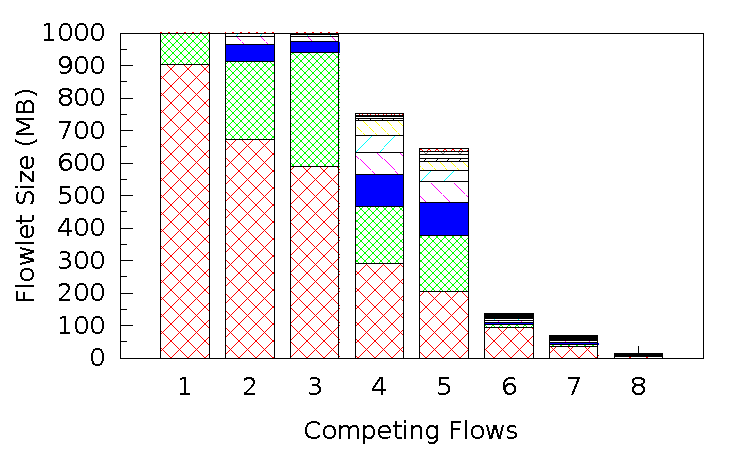
\includegraphics[width=0.55\textwidth]{./figures/presto/flowlets/histo.pdf}
        \caption{Stacked histogram of flowlet sizes (in MB) for a 1 GB {\tt scp} file transfer. We vary the number of {\tt nuttcp} background flows and
                denote them as {\em Competing Flows}. The size of each flowlet is shown within each bar, and flowlets
                are created whenever there is a 500 $\mu$s delay between segments. The top 10 flowlet sizes are shown here.
                We also analyzed the results of a 1 GB {\tt nuttcp}, {\tt ftp}, and a simple custom client/server transfer and found them
                to be similar. }
        \label{micro_flowlet_size}
\end{figure}


Another possibility is to load balance on flowlets~\cite{alizadeh2014conga,juniper-vcf}.  
A flow is comprised of a series of bursts, and a flowlet is created when
the inter-arrival time between two packets in a flow exceeds a threshold inactivity timer.  
In practice, inactivity timer values are between 100-500 $\mu$s~\cite{alizadeh2014conga}. 
These values intend to strike a good balance between load balancing on a sub-flow level 
and acting as a buffer to limit reordering between flowlets.
Flowlets are derived from traffic patterns at the sender, and in practice this
means the distribution of flowlet sizes is not uniform. To analyze flowlet sizes, a simple experiment is shown in Figure~\ref{micro_flowlet_size}. 
We connect a sender and a receiver to a single switch and start an {\tt scp} transfer designed to 
emulate an elephant flow. Meanwhile, other senders are hooked up to the same switch and
send to the same receiver. We vary the number of these competing flows and show a stacked histogram of 
the top 10 flowlet sizes for a 1 GB {\tt scp} transfer with a 500 $\mu$s inactivity timer. 
The graph shows flowlet sizes can be quite large, with more than half the transfer being attributed
to a single flowlet for up to 3 competing flows. Using a smaller inactivity timer, such 100$\mu$s, helps (90\% of flowlet sizes are 114KB or less), but
does not prevent a long tail: 0.1\% of flowlets are larger than 1 MB, with the largest ranging from 2.1-20.5 MB.
Collisions on large flowlet sizes can lead to congestion.
The second problem with flowlets is that small inactivity thresholds, such as 100 $\mu$s, can lead to significant reordering.
Not only does this impact TCP performance (profiled in \secref{sec:presto-eval}), 
but it also needlessly 
breaks small flows into several flowlets. With only one flow in the network, we found a 50 KB
mice flow was broken into 4-5 flowlets on average. Small flows typically do not need to be
load balanced on a sub-flow level and need not be exposed to reordering.


The shortcomings of the previous approaches lead us to reconsider on what granularity
load balancing should occur. 
Ideally, sub-flow load balancing should be done on near uniform sizes.
Also, the unit of load balancing should be small to
allow for fine-grained load balancing, but not so small as to break small flows into 
many pieces or as to be a significant computational burden. As a result, we
propose load balancing on 64 KB units of data we call {\em flowcells}. Flowcells
have a number of advantages. First, the maximum segment size supported by TSO
is 64 KB, so flowcells provide a natural interface to high speed optimizations provided
by the NIC and OS and can scale to fast networking speeds. Second, an overwhelming fraction of mice flows are less than 64 KB in size
 and thus do not have to worry about reordering~\cite{benson10,vl2,kandula2009nature}.
Last, since most bytes in datacenter networks originate from elephant flows~\cite{kandula2009nature,benson10,alizadeh2011dctcp},
this ensures that a significant portion of datacenter traffic is routed on uniform
sizes. While promising, this approach must combat reordering to be effective. 
Essentially we make a trade-off: we provide line rate load balancing in the most effective
manner as to avoid congestion and then handle reordering head-on at the receiver.

\tightparagraph{End-to-End vs Per-Hop Multipathing}
The last design consideration is whether multipathing should be done on a local, per-hop level (\eg{}, ECMP), or
on a global, end-to-end level. In Presto, we choose the latter: pre-configured end-to-end paths
are allocated in the network and path selection (and thus multipathing) is realized by having the network edge
place flowcells onto these paths. 
Presto can be used to load-balance in an ECMP style per-hop manner but the choice of end-to-end 
multipathing provides additional benefits due to greater control on how flowcells are mapped to
paths. Per-hop multipathing can be inefficient
under asymmetric topologies~\cite{zhou2014wcmp}, and load-balancing on a global end-to-end level can allow
for weighted scheduling at vSwitch to rebalance traffic. This is especially important when failure occurs.
The second benefit is that flowcells can be assigned over multiple paths very evenly
by iterating over paths in a round-robin, rather than randomized, fashion. 

\subsubsection{Reordering Challenges}
Due to the impact of fine-grained, flowcell-based load balancing, Presto must account for reordering. Here, we 
highlight reordering challenges. The next section shows how Presto deals with these concerns.

\tightparagraph{Reordering's Impact on TCP} The impact of reordering on TCP is well-studied~\cite{leung2007overview,paxson1997end}. 
Duplicate acknowledgments caused by reordering
can cause TCP to move to a more conservative sender state and reduce the sender's congestion window.
Relying on parameter tuning, such as adjusting the DUP-ACK threshold, is not ideal because 
increasing the DUP-ACK threshold increases the time to recover from real loss. Other TCP settings
such as Forward Acknowledgement (FACK) assume un-acked bytes in the SACK are lost and degrade
performance under reordering. 
A scheme that introduces reordering should not rely on careful configuration of TCP parameters
because (i) it is hard to find a single set of parameters that work effectively over multiple 
scenarios and (ii) datacenter tenants should not be forced to constantly tune their networking stacks.
Finally, many reordering-robust variants of TCP have been proposed~\cite{rr-tcp,blanton2002making,tcp-pr}, but
as we will show, GRO becomes ineffective under reordering. Therefore, reordering should
be handled below the transport layer.

\tightparagraph{Computational Bottleneck of Reordering}
Akin to TSO, Generic Receive Offload (GRO) mitigates the computational burden of receiving
1500 byte packets at 10 Gbps. GRO is implemented in the kernel of the hypervisor
and its handler is called directly by the NIC driver. It is responsible
for aggregating packets into larger segments that are pushed up to OVS and the TCP/IP stack.
Because modern CPUs use aggressive prefetching, the cost of receiving
TCP data is now dominated by per-packet, rather than per-byte, operations.
As shown by Menon~\cite{optimize-tcp-receive},  the majority of this overhead comes from
buffer management and other routines not related to protocol processing, and therefore 
significant computational overhead can be avoided by aggregating "raw" packets from
the NIC into a single {\tt sk\_buff}.\footnote{Refer to~\cite{optimize-tcp-receive} for detailed study and explanation}
Essentially, spending a few cycles to aggregate packets within GRO creates less segments for
TCP and prevents having to use substantially more cycles at higher layers in the networking stack.

To better understand the problems reordering causes, a brief description of  
the TCP receive chain in Linux follows. First, interrupt coalescing
essentially allows the NIC to create an interrupt for a batch of packets~\cite{mogul1997eliminating,understanding-linux-network},
which prompts the driver to poll the packets into an aggregation queue. Next, the driver
invokes the GRO handler, located in the kernel, which
{\em merges} the packets into larger segments. The merging continues,
possibly across many polling events, until a segment
reaches a threshold size, a certain age, or cannot be combined with the incoming packet. Then, the
combined, larger segment is {\em pushed up} to the rest of the TCP/IP networking stack. The GRO process is
done on a per-flow level. With GRO disabled, throughput drops to around
5.7-7.1 Gbps and CPU utilization spikes to 100\% (\secref{sec:presto-eval} and~\cite{bullettrains}). 
Receive offload algorithms, whether in hardware 
(LRO)~\cite{grossman2005large} or in software (GRO), are usually
{\em stateless} to make them fast: no state is kept beyond the segment being merged.


\begin{figure}[t]
        \centering
  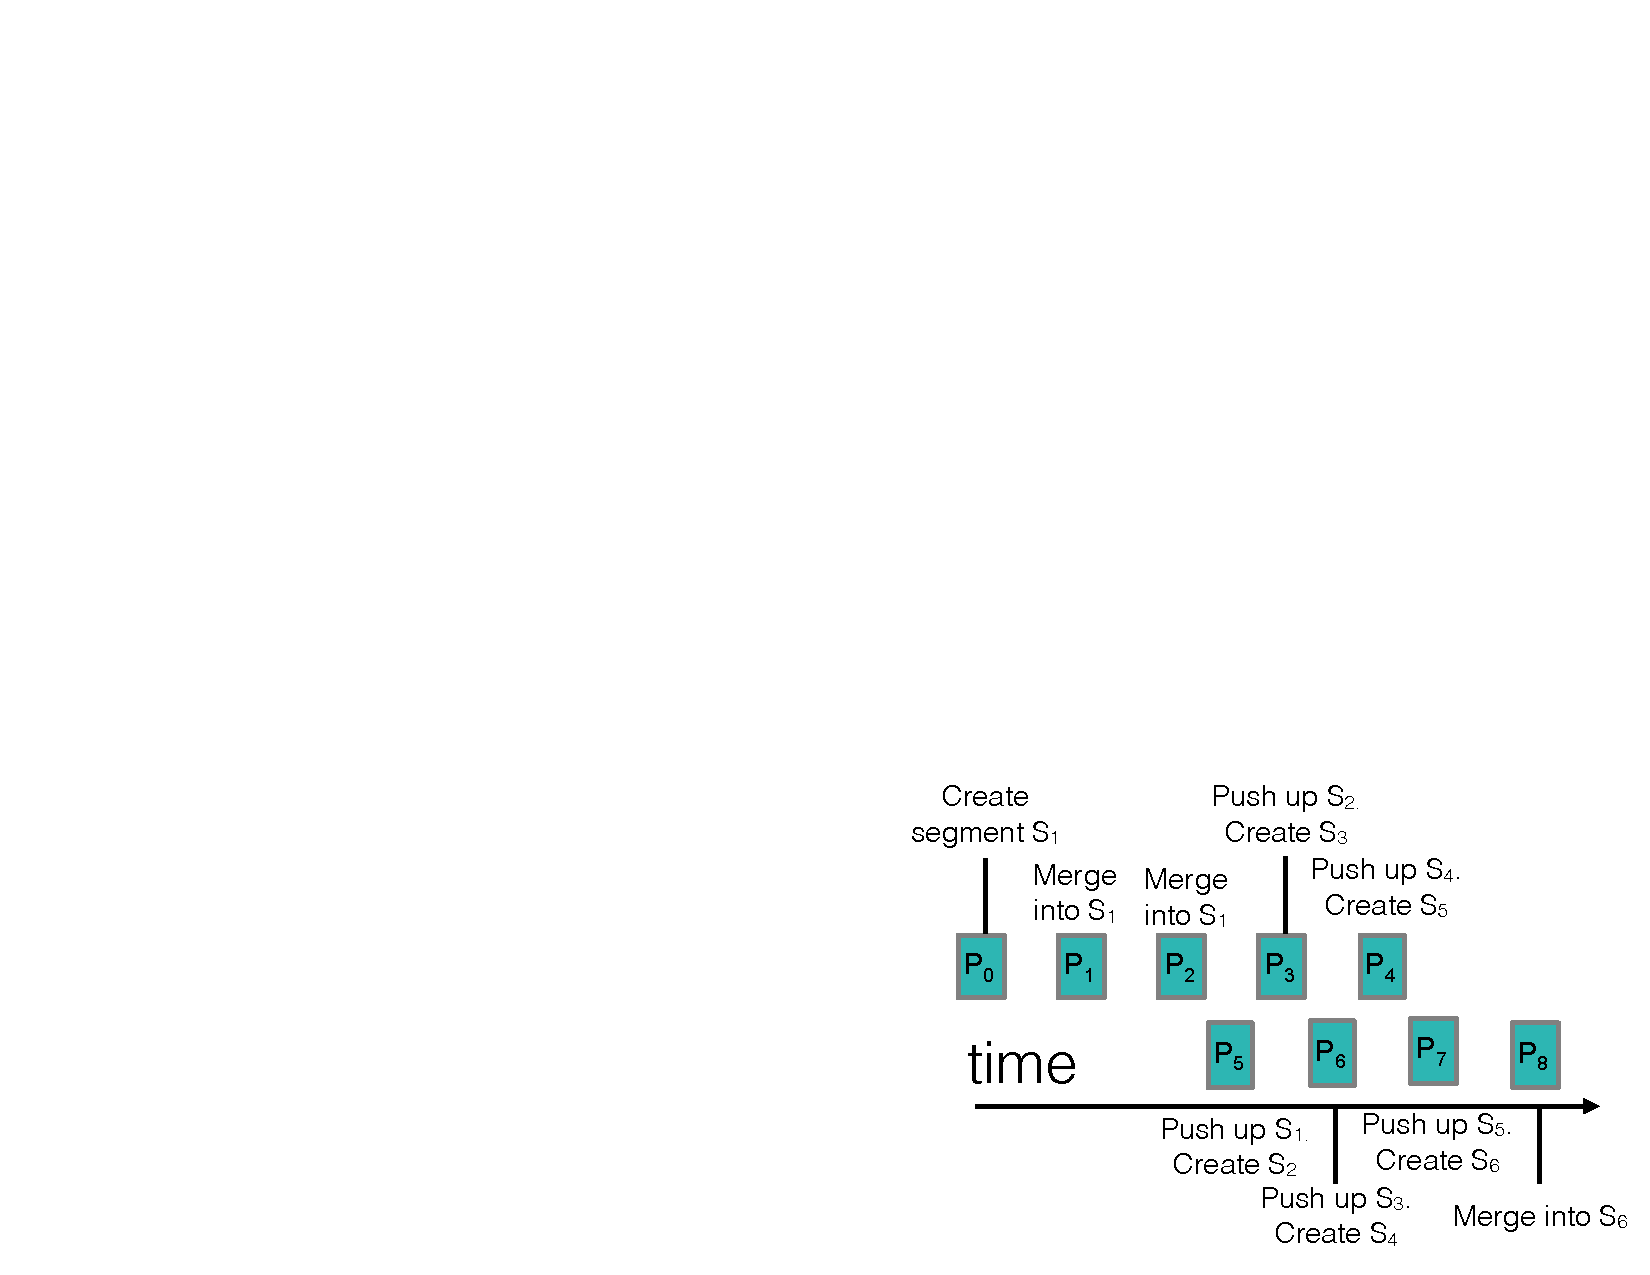
\includegraphics[width=0.55\textwidth]{./figures/presto/gro-design/gro-break.pdf}
        \caption{GRO pushes up small segments ($S_i$) during reordering.}
        \label{gro-break}
\end{figure}


We now uncover how GRO breaks down in the face of reordering. Figure~\ref{gro-break} shows the impact of reordering on GRO.  Reordering does not allow the segment to grow: each reordered packet cannot be merged with the existing segment, and thus the previously created segment must be pushed up. With extreme reordering, GRO is effectively disabled because small MTU-sized segments are constantly pushed up. This causes (i) severe computational overhead and (ii) TCP to be exposed to significant amounts of reordering. We term this the {\em small segment flooding} problem.

Determining where to combat the reordering problem has not previously taken the small segment flooding problem into account.  Using a reordering buffer to deal with reordered packets is a common solution (\eg{}, TCP does this, other works re-sort in a shim layer below TCP~\cite{cao2013drb}), but a buffer implemented above GRO cannot prevent small segment flooding.  Implementing a buffer below GRO means that the NIC must be changed, which is (i) expensive and cumbersome to update and (ii) unlikely to help combat reordering over multiple interrupts.

In our system, the buffer is implemented in the GRO layer itself.  We argue this is a natural location because GRO can
directly control segment sizes while simultaneously limiting the impact of reordering. 
Furthermore, GRO can still be applied on packets pushed up from LRO, which means hardware doesn't have to be modified
or made complex.
Implementing a better GRO has multiple challenges. The algorithm should be fast and light-weight to scale to fast networking speeds. Furthermore, an ideal scheme should be able to distinguish loss from reordering.  When a gap in sequence numbers is detected (\eg{}, when $P_5$ is received after $P_2$ in Figure~\ref{gro-break}), it is not obvious if this gap is caused from loss or reordering.  If the gap is due to reordering, GRO should not push segments up in order to try to wait to receive the missing gap and merge the missing packets into a preestablished segment.  If the gap is due to loss, however, then GRO should immediately push up the segments to allow TCP to react to the loss as fast as possible. Ideally, an updated GRO algorithm should ensure TCP does not perform any worse than a scheme with no reordering. Finally, the scheme should adapt to prevailing network conditions, traffic patterns and application demands.



\subsection{Design}
\label{sec:presto-design}

This section presents the design of Presto by detailing
the sender, the receiver, and how the network
adapts in the case of failures and asymmetry.

\begin{figure}[!t]
        \centering
  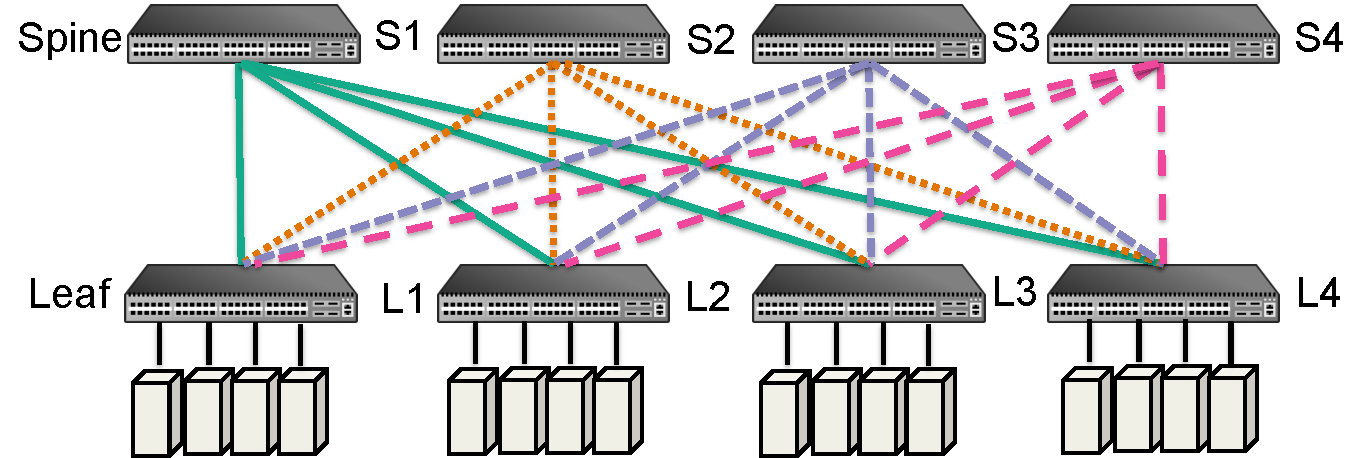
\includegraphics[width=0.55\textwidth,height=0.17\textwidth]{./figures/presto/macro/macro_evaluation_topology_refined.pdf}
        \caption{Our testbed: 2-tier Clos network with 16 hosts.}
        \label{macro_evaluation_topology}
\end{figure}

\subsubsection{Sender}


\tightparagraph{Global Load Balancing at the Network Edge}
In Presto, a centralized controller is employed to collect the
network topology and disseminate corresponding load balancing information to the edge vSwitches. 
The goal of this design is to ensure the vSwitches, as a whole, can load balance the network
in an even fashion, but without requiring an individual vSwitch to have detailed information
about the network topology, updated traffic matrices or strict coordination amongst senders.
 At a high level, the controller partitions
the network into a set of multiple spanning trees. Then, the controller
assigns each vSwitch a unique forwarding label in each spanning tree.
By having the vSwitches partition traffic over these spanning trees in a fine-grained
manner, the network can load balance traffic in a near-optimal fashion.

The process of creating spanning trees is made simple by employing multi-stage Clos
networks commonly found in datacenters. For example, in a 2-tier Clos network
with $\nu$ spine switches, the controller can easily allocate $\nu$ disjoint spanning
trees by having each spanning tree route through a unique spine switch. Figure~\ref{macro_evaluation_topology}
shows an example with four spine switches and four corresponding disjoint spanning trees.
When there are $\gamma$ links between each spine and leaf switch in a 2-tier Clos network,
the controller can allocate $\gamma$ spanning trees per spine switch.
Note that 2-tier Clos networks are scalable because they easily support a large number
of hosts with only a few high density spine switches~\cite{alizadeh2014conga}.
In general, the controller ensures links in the network are equally covered
by the allocated spanning trees.
Once the spanning trees are created, the controller assigns a unique forwarding label
for each vSwitch in every spanning tree and installs them into the network.
Forwarding labels can be implemented in a variety of ways using
technologies commonly deployed to forward on labels,
such as MPLS~\cite{casado2012fabric}, VXLAN~\cite{alizadeh2014conga,koponen2014network}, 
or IP encapsulation~\cite{cao2013drb}. 
In Presto,
label switching is implemented with shadow MACs~\cite{shadow-mac}. 
Shadow MACs implement label-switching for commodity Ethernet by using the 
destination MAC address as an opaque forwarding label that can easily be 
installed in L2 tables. 
Each vSwitch is assigned one shadow MAC per spanning tree.
Note Shadow MACs are extremely scalable on
existing chipsets because they utilize the large L2 forwarding table. For example,
Trident II-based switches~\cite{bcm-smart-table} have 288k L2 table entries and 
thus 8-way multipathing (\ie{}, each vSwitch has 8 disjoint spanning trees)
can scale up to 36,000 physical servers.


\tightparagraph{Load Balancing at the Sender}
After the controller installs the shadow MAC forwarding rules into the network, it creates a mapping
from each physical destination MAC address to a list of corresponding shadow MAC addresses. These mappings
provide a way to send traffic to a specific destination over different spanning trees. 
The mappings are pushed from the controller to each vSwitch in the network, either on-demand or preemptively.
In Presto, the vSwitch on the sender monitors outgoing traffic (\ie{}, maintains a per-flow counter in the datapath) 
and rewrites the destination MAC
address with one of the corresponding shadow MAC addresses.
The vSwitch assigns the same shadow MAC address to all consecutive segments until the 64 KB limit is reached.
In order to load balance the network effectively, the vSwitch 
iterates through destination shadow MAC addresses in a round-robin fashion. 
This allows the edge vSwitch to load balance over the network in a very fine-grained fashion.

Sending each 64 KB worth of flowcells over a different path in the network can cause reordering and must
be carefully addressed.
To assist with reordering at the receiver (Presto's mechanisms for combatting reordering are detailed in the next section), 
the sender also includes a sequentially increasing {\em flowcell ID} into each segment.
For example, 
in our setup the controller installs forwarding rules solely on the destination MAC address.
ARP is handled in a centralized manner, so
the source MAC address can be used to hold the flowcell ID. Other options are possible, 
\eg{}, some schemes include load balancing metadata in the reserved bits of the 
VXLAN header~\cite{presto-nvo3}.\footnote{In our
implementation, TCP options hold the flowcell ID for simplicity and ease of debugging.}
Note that since the flowcell ID and the shadow MAC address are modified before a segment is handed to the NIC,
the TSO algorithm in the NIC replicates these values to all derived MTU-sized packets.

\begin{algorithm}[t]
\caption{Pseudo-code of Presto GRO {\tt flush} function}
\label{alg:gro}
\begin{algorithmic}[1]
%\REQUIRE $n \geq 0 \vee x \neq 0$
%\ENSURE $y = x^n$
\FOR{each flow f}
\FOR{$S \in f.{\tt segment\_list}$}
%\STATE f = getFlow(S)
\IF{f.lastFlowcell == getFlowcell(S)}
\STATE f.expSeq $\leftarrow$ max(f.expSeq, S.endSeq)
\STATE pushUp(S)
\ELSIF{getFlowcell(S) $>$ f.lastFlowcell}
\IF{f.expSeq == S.startSeq}
\STATE f.lastFlowcell $\leftarrow$ getFlowcell(S)
\STATE f.expSeq $\leftarrow$ S.endSeq
\STATE pushUp(S)
\ELSIF{timeout(S)}
\STATE f.lastFlowcell $\leftarrow$ getFlowcell(S)
\STATE f.expSeq $\leftarrow$ S.endSeq
\STATE pushUp(S)
\ENDIF
\ELSE
\STATE pushUp(S)
\ENDIF
\ENDFOR
\ENDFOR
\end{algorithmic}
\end{algorithm}

\subsubsection{Receiver}
The main challenge at the receiver is dealing with reordering that can occur when different flowcells
are sent over different paths. The high level goal of our receiver implementation is
to mitigate the effects of the small segment flooding problem by (i) not so aggressively pushing
up segments if they cannot be merged with an incoming packet and (ii) ensuring that segments
pushed up are delivered in order.

\tightparagraph{Mitigating Small Segment Flooding} Let's use Figure~\ref{gro-break} as a motivating example 
on how to combat the small segment flooding problem. Say a polling event has occurred, and the driver retrieves
9 packets from the NIC ($P_0$-$P_8$). The driver calls the GRO handler, which tries to merge consecutive packets
into larger segments. The first three packets ($P_0$-$P_2$) are merged into a segment, call it $S_1$ (note: in practice
$S_1$ already contains in order packets received before $P_0$).
When $P_5$ arrives, a new segment $S_2$, containing $P_5$, should be created. Instead of pushing up $S_1$ (as is done currently),
both segments should be kept.
Then, when $P_3$ is received, it can be merged into $S_1$. Similarly, $P_6$ can be merged into $S_2$. This process
can continue until $P_4$ is merged into $S_1$. At this point, the gap between the original out-of-order reception ($P_2$-$P_5$)
 has been filled, and $S_1$ can be pushed up and $S_2$ can continue to grow. This means the size of the segments being pushed up is increased,
and TCP is not exposed to reordering.

The current default GRO algorithm works as follows. An interrupt by the NIC causes the driver to poll
(multiple) packets from the NIC's ring buffer. The driver calls the GRO handler on the received batch
of packets. GRO keeps a simple doubly linked list, called {\tt gro\_list}, that contains 
segments, with a flow having at most one segment in the list. When packets for a flow are
received in-order, each packet can be merged into the flow's preexisting segment. When a packet
cannot be merged, such as with reordering, the corresponding segment is pushed up (ejected from the
linked list and pushed up the networking stack) and a new segment is created from the packet. 
This process is continued until all packets in the batch are serviced. At the end 
of the polling event, a {\tt flush} function is called that pushes up all segments in the
{\tt gro\_list}.

Our GRO algorithm makes the following high-level changes. First, multiple segments can be
kept per flow, and each flow contains a doubly linked list of its segments (called {\tt segment\_list}). 
To ensure the merging process is fast each linked list is kept in a hash table (keyed on flow).
When an incoming packet cannot be merged with any existing segment, the existing
segments are kept and a new segment is created from the packet.
New segments are added to the head of the linked list so that merging subsequent packets is typically $\mathcal{O}(1)$.
When the merging is completed over all packets in the batch, the {\tt flush} function is called. 
The {\tt flush} function decides whether to push segments up or to keep them. Segments may 
be kept so reordered packets still in flight have enough time to arrive and can then be placed in order
before being pushed up. 
Reordering can cause the linked lists to become slightly out-of-order, so
at the beginning of {\tt flush} an insertion sort is run to help easily decide if segments are in order.

The pseudo-code of our {\tt flush} function is presented in Algorithm~\ref{alg:gro}.
For each flow, our algorithm keeps track of the next expected in-order
sequence number ({\tt f.expSeq}) and the corresponding flowcell ID
of the most recently received in-order sequence number ({\tt f.lastFlowcell}).
The {\tt flush} function iterates over 
the sorted segments ($S$), from lowest sequence number to highest sequence number, in the {\tt segment\_list} (line 2).
The rest of the code is presented in the subsections that follow.


\tightparagraph{How to Differentiate Loss from Reordering?} 
In the case of no loss or reordering, our algorithm keeps pushing up segments and updating state. Lines 3-5
deal with segments from the same flowcell ID, so we just need to update {\tt f.expSeq} each time. Lines 
6-10 represent the case when the current flowcell ID is fully received and we start to receive the
next flowcell ID. The problem, however, is when there is 
a gap that appears between the sequence numbers of the segments. When a gap is encountered,
it isn't clear if it is caused from reordering or from loss. If the gap is due to reordering,
our algorithm should be conservative and try to wait to receive the packets that "fill in the gap" 
before pushing segments up to TCP. If the gap is due to loss, however, then we should push up the 
segments immediately so that TCP can react to the loss as quickly as possible.

To solve this problem, we leverage the fact that all packets carrying the same flowcell ID traverse the 
same path and should be in order.
This means incoming sequence numbers can be monitored to check for
gaps. A sequence number gap within the same flowcell ID is assumed to be a loss, and not reordering,
so those packets are pushed up immediately (lines 3-5).
Note that because a flowcell consists of many packets (a 64KB flowcell consists
of roughly 42 1500 byte packets), when there is a loss, it is likely that it occurs within flowcell boundaries. 
The corner case, when a gap occurs on the flowcell boundary, leads us to the next design question.

\tightparagraph{How to Handle Gaps at Flowcell Boundaries?}
When a gap is detected in sequence numbers at flowcell boundaries, it is not clear if the gap is due
to loss or reordering. Therefore, the segment should be held long enough to
handle reasonable amounts of reordering, but not so long that TCP cannot respond
to loss promptly. Previous approaches that deal with reordering typically employ a large static
timeout (10ms)~\cite{cao2013drb}. 
Setting the timeout artificially high can handle reordering, but hinders TCP when the gap is
due to loss. 
Setting a lower timeout is difficult because it depends on many dynamic factors such as delays between
segments at the sender, amount of network congestion in different paths, and traffic patterns (multiple flows 
received at the same NIC affect inter-arrival time). 
As a result, we devise an adaptive timeout scheme, which monitors recent reordering events and sets a dynamic timeout value accordingly.
Presto tracks cases when there is reordering, but no loss, on flowcell boundaries and keeps an exponentially-weighted
moving average ($EWMA$) over these times. Presto then applies a timeout of $\alpha * EWMA$ to a segment when a gap is 
detected on flowcell boundaries. 
Here $\alpha$ is an empirical parameter that allows for timeouts to grow. As a further optimization, if a segment
has timed out, but a packet has been merged into that segment in the last $\frac{1}{\beta} * EWMA$ time interval, then 
the segment is still held in hopes of preventing reordering. We find $\alpha$ and $\beta$
work over a wide range of parameters and set both of them to 2 in our experiments. A timeout firing is dealt with in lines 11-15.


\subsubsection{Failure Handling and Asymmetry}
When failures occur, Presto relies on the controller to update the forwarding
behavior of the affected vSwitches. The controller can simply prune the spanning
trees that are affected by the failure, or more generally enforce a weighted
scheduling algorithm over the spanning trees.
Weighting allows for Presto to evenly distribute traffic over an asymmetric topology.
Path weights can be implemented in a simple fashion by duplicating shadow MACs used in
the vSwitch's round robin scheduling algorithm.
For example, assume we have three paths in total ($p_1$, $p_2$ and $p_3$) and their updated weights are 0.25, 0.5 and 0.25 respectively.
Then the controller can send the sequence of $p_1$, $p_2$, $p_3$, $p_2$ to the vSwitch, which
can then schedule traffic over this sequence in a round robin fashion to realize the new path weights.
This way of approximating path weights in the face of network
asymmetry is similar to WCMP~\cite{zhou2014wcmp}, but instead of having to change switch firmware and use
scarce on-chip SRAM/TCAM entries, we can push the weighted load balancing entirely to the network edge.

As an added optimization, Presto can leverage any fast failover features that 
the network supports, such as BGP fast external failover, MPLS fast reroute, or OpenFlow failover groups. Fast failover detects port failure and can move corresponding traffic
to a predetermined backup port.
\footnote{Hardware failover latency ranges from several to 
tens of milliseconds}
This ensures traffic is moved away from the failure rapidly and the network
remains connected when redundant links are available.
Moving to backup links causes imbalance in the network,
so Presto relies on the controller learning of the network change, computing weighted multipath schedules, and
disseminating the schedules to the vSwitches. 


\subsection{Methodology}
\label{sec:presto-method}

\tightparagraph{Implementation}
We implemented Presto in Open vSwitch v2.1.2 and Linux kernel v3.11.0.
In OVS, we modified 5 files and $\sim$600 lines of code. For GRO, we modified 11 files and $\sim$900 lines of code.

\tightparagraph{Testbed} We conducted our experiments on a physical
testbed consisting of 16 IBM System x3620 M3 servers with 6-core Intel Xeon
2.53GHz CPUs, 60GB memory, and Mellanox ConnectX-2 EN 10GbE NICs. 
The servers were connected in a 2-tier Clos network topology with 10Gbps
IBM RackSwitch G8264 switches, as shown in Figure~\ref{macro_evaluation_topology}.

\tightparagraph{Experiment Settings}
We ran the default TCP implementation in the Linux kernel (TCP CUBIC)
and set {\tt tcp\_sack}, {\tt tcp\_fack}, {\tt tcp\_low\_latency} to 1 unless otherwise noted. 
Further, we tuned the host RSS and IRQ affinity settings and kept them the same in all experiments.

\tightparagraph{Workloads}
We evaluate Presto with a set of synthetic and realistic workloads. 
Similar to previous works~\cite{al2010hedera,rasley2014planck}, 
our synthetic workloads include:

{\em Shuffle}: Each server in the testbed sends 1GB data to every other server in the testbed in random order. 
Each host sends two flows at a time. %The shuffle is finished if all the servers have finished their jobs. 
This workload emulates the shuffle behavior of MapReduce/Hadoop workloads.

{\em Stride(8)}: We index the servers in the testbed from left to right. In stride(8) workload, server[i] sends to server[(i+8) mod 16].

{\em Random}: Each server sends to a random destination 
 not in the same pod as itself. Multiple senders can send to the same receiver.

{\em Random Bijection}: Each server sends to a random destination not in the same pod as itself. 
Different from random, each server only receives data from one sender.
 
Finally, we also evaluate Presto with trace-driven workloads from real datacenter traffic~\cite{kandula2009nature}.

\tightparagraph{Performance Evaluation}
We compare Presto to ECMP, MPTCP, and a 
single non-blocking switch used to represent an optimal scenario.
ECMP is implemented by enumerating all possible end-to-end paths and randomly selecting a path for each flow.
MPTCP uses ECMP to determine the paths of each of its sub-flows.
The MPTCP implementation is still under active development, and
we spent significant effort in finding the most stable configuration of MPTCP on our testbed. Ultimately, we found that Mellanox {\tt mlx\_en4} driver version
2.2, MPTCP version 0.88, subflow count set to 8, OLIA congestion control algorithm, and configured buffer sizes
as recommended by~\cite{dc-mptcp} gave us the best trade-offs in terms of throughput, latency, loss and stability.
Unfortunately, despite our efforts, we still occasionally witness some stability issues 
with MPTCP that we believe are due to implementation bugs.

We evaluate Presto on various performance metrics, including: 
throughput (measured by {\tt nuttcp}), 
round trip time (a single TCP packet, measured by {\tt sockperf}), 
mice flow completion time (time to send a 50 KB flow and receive an application-layer acknowledgement), packet loss (measured from switch counters), 
and fairness (Jain's fairness index over flow throughputs).  Mice flows are sent every 100 ms and elephant flows last 10 seconds. 
Each experiment is run for 10 seconds over 20 runs. Error bars on graphs denote
the highest and lowest value over all runs.


%\subsection{Microbenchmarks}
\label{sec:presto-micro}

We first evaluate the effectiveness of Presto over a series of microbenchmarks. Using 
canonical topologies, we investigate (i) Presto's effectiveness in preventing the small segment
flooding problem and reordering, (ii) Presto's CPU overhead, (iii) Presto's ability to scale
to multiple paths, (iv) Presto's ability to handle congestion, (v) comparison to flowlet
switching, and (vi) comparison to local, per-hop load balancing.

%%%%%micro test - scalability and congestion test topology
\begin{figure}[t]
        \centering
	\begin{subfigure}[b]{0.40\textwidth}
        	\centering
  		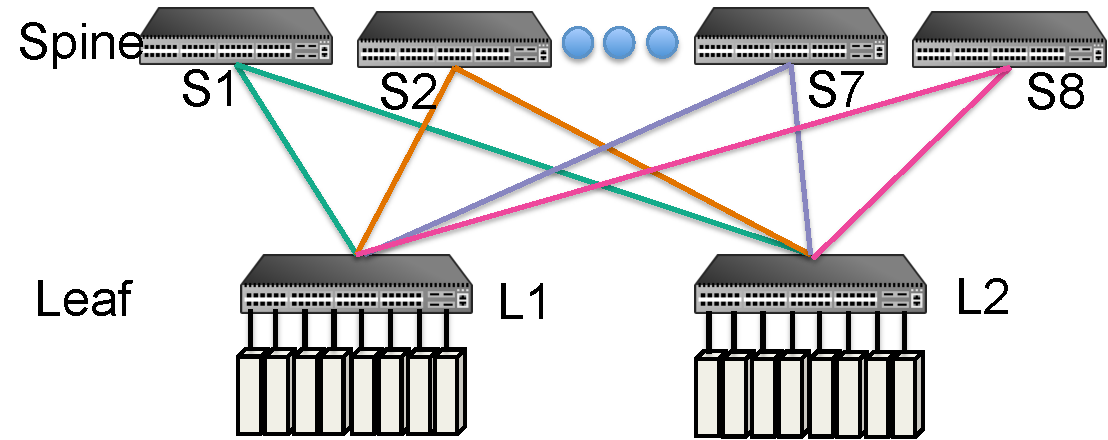
\includegraphics[width=\textwidth]{./figures/presto/micro_test_topology/micro_scalabilitytest_topology_refined.pdf}
        	\caption{}
		\label{micro_scalability_topology}
	\end{subfigure}
	\begin{subfigure}[b]{0.40\textwidth}
                \centering
		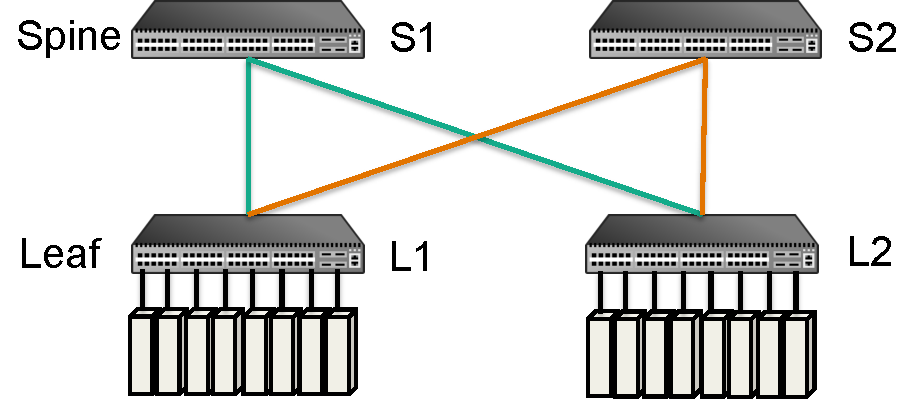
\includegraphics[width=\textwidth]{./figures/presto/micro_test_topology/micro_congestiontest_topology_refined.pdf}
        	\caption{}
		\label{micro_congestion_topology}
	\end{subfigure}
	\caption{(a) Scalability benchmark and (b) Oversubscription benchmark topology.}
	\label{micro_topology}
\end{figure}

%%%%%gro effectiveness shows
\begin{figure}[t]
	\centering
	\begin{subfigure}[b]{0.35\textwidth}
                \centering
  		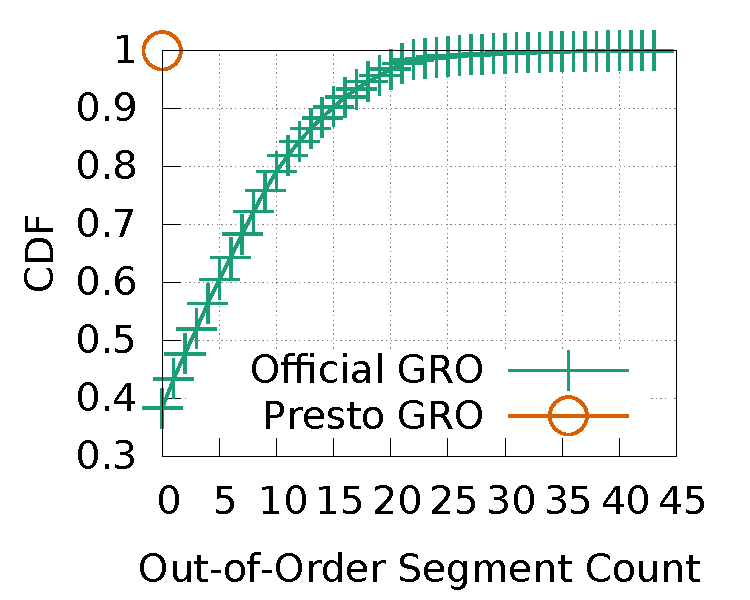
\includegraphics[width=\textwidth]{./figures/presto/gro_effectiveness/metric1_seg_cdf_compare.pdf}
		\caption{}
		\label{gro_effectiveness_on_reordering}
	\end{subfigure}
        \begin{subfigure}[b]{0.35\textwidth}
                \centering
		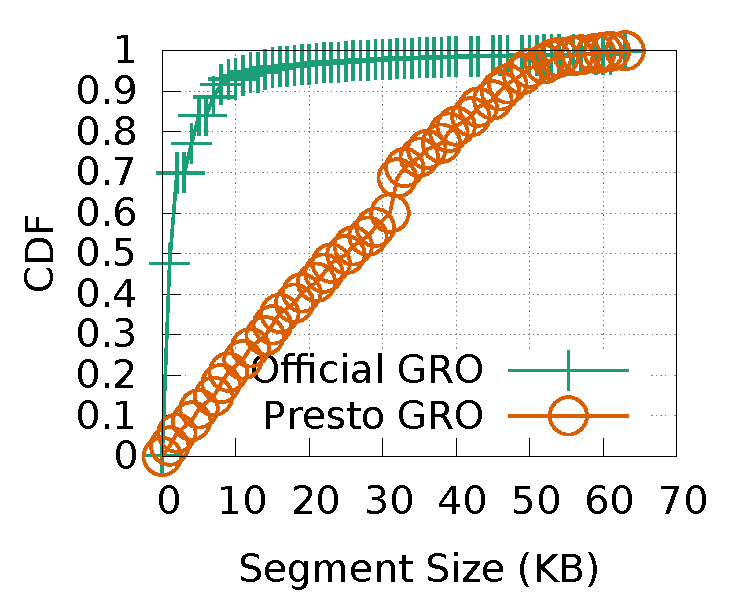
\includegraphics[width=\textwidth]{./figures/presto/gro_effectiveness/metric1_pktsize_cdf_compare.pdf}
        	\caption{}
		\label{gro_effectiveness_on_pktsize}
	\end{subfigure}
	\caption{(a) Illustration of the modified GRO's effectiveness on masking reordering. 
		(b) In case of massive packet reordering, official GRO cannot merge packets effectively such that lots of small
                packets are processed by TCP which poses great processing overhead for CPU.}
	\label{gro_effectiveness}
\end{figure}

\tightparagraph{Presto's GRO Combats Reordering}
To examine Presto's ability to handle packet reordering, we perform a simple experiment
on topology shown in Figure~\ref{micro_congestion_topology}.
Here two servers attached to leaf switch L1 
send traffic to their own receivers attached to leaf switch L2
by spreading 64KB flowcells over the two network paths. 
This setup can cause reordering for each flow, so 
we compare Presto's GRO to
an unmodified GRO, denoted "Official GRO". 
The amount of reordering exposed to TCP is presented in Figure~\ref{gro_effectiveness_on_reordering}.
To quantify packet reordering, we show a CDF of the {\em out-of-order segment count}:~\ie{},
the number of segments from other flowcells between the first packet and last packet of each flowcell. A value of zero
means there is no reordering and larger values mean more reordering. The figure shows Presto's GRO can completely mask reordering
while official GRO incurs significant reordering. As shown in Section~\ref{sec:presto-background}, reordering can
also cause smaller segments to be pushed up the networking stack, causing significant processing overhead.
Figure~\ref{gro_effectiveness_on_pktsize} shows the received TCP segment size distribution.  Presto's GRO
pushes up large segments, while the official GRO pushes up many small segments.
The average TCP throughputs in official GRO and Presto GRO are 4.6Gbps (with 86\% CPU utilization) and 
9.3Gbps (with 69\% CPU utilization), respectively. Despite the fact that official GRO only obtains 
about half the throughput of Presto's GRO, it still incurs more than 24\% higher CPU overhead. 
Therefore, an effective scheme must deal with both reordering and small segment overhead.

\begin{figure}[t]
        \centering
  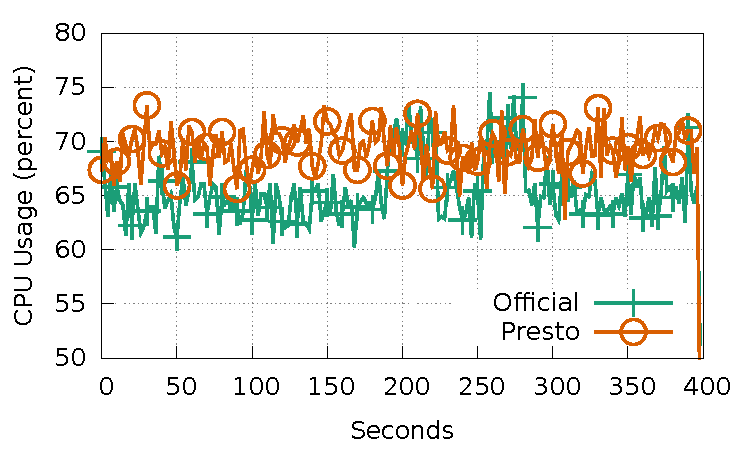
\includegraphics[width=0.55\textwidth]{./figures/presto/mornitor_cpu/macro_compare_cpu_usage.pdf}
        \caption{Presto incurs 6\% CPU overhead on average.}
        \label{micro_compare_cpu}
\end{figure}

\tightparagraph{Presto Imposes Limited CPU Overhead}
We investigate Presto's CPU usage by
running the stride workload on a 2-tier Clos network as shown in Figure~\ref{macro_evaluation_topology}. 
For comparison, official GRO is run with the stride workload using a non-blocking switch (so there
is no reordering). Note both official GRO and Presto GRO can achieve 9.3Gbps.  
The receiver CPU usage is sampled every 2 seconds over a 400 second interval, and
the time-series is shown in Figure~\ref{micro_compare_cpu}. 
On average, Presto GRO only increases CPU usage by 6\% compared with the official GRO. 
The minimal CPU overhead comes from Presto's careful design and implementation. 
At the sender, Presto needs just two {\tt memcpy} operations (1 for shadow MAC rewriting, 1 for flowcell ID encoding). 
At the receiver, Presto needs one {\tt memcpy} to rewrite the shadow MAC back to the real MAC and
also incurs slight overhead because multiple segments are now kept per flow. The overhead
of the latter is reduced because these segments are largely kept in reverse sorted order, which means {\tt merge}
on an incoming packet is usually $\mathcal{O}(1)$. The insertion sort is done at the beginning of each {\tt flush} event over a small
number of mostly in-order segments, which easily amortizes overhead because it is called infrequently compared to {\tt merge}.


\begin{figure}[t]
        \centering
  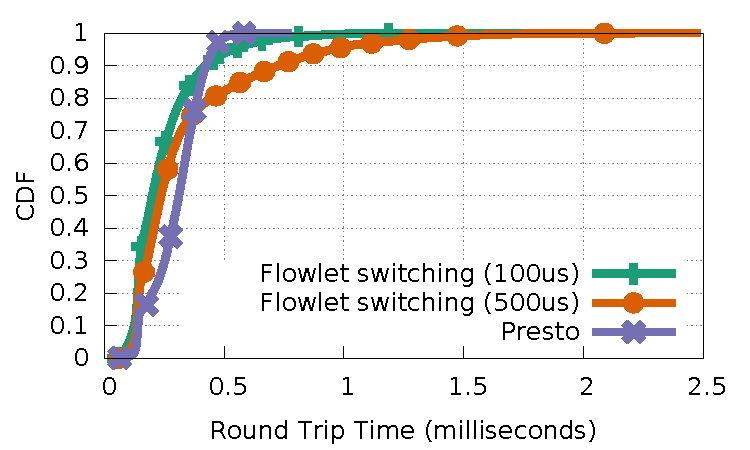
\includegraphics[width=0.55\textwidth]{./figures/presto/flowlets/flowlet_switching/flowlet_presto_compare_sockperf.pdf}
        \caption{Round trip time comparison of Flowlet switching~\cite{flowlet,alizadeh2014conga} and Presto in Stride workload. 
		The throughputs of Flowlet switching with 100 $\mu\text{s}$ gap, 500 $\mu\text{s}$ gap and Presto 
		are 4.3Gbps, 7.6Gbps and 9.3Gbps respectively. }
        \label{micro_flowlet_rtt_compare}
\end{figure}


\tightparagraph{Comparison to Flowlet Switching}
We implemented a flowlet load-balancing scheme in OVS that detects
inactivity gaps and then schedules flowlets over disjoint paths in a round robin fashion
(Presto does this over flowcells instead of flowlets).
The receiver for flowlets uses official GRO.
Presto is compared to 500 $\mu$s and 100 $\mu$s inactivity timers in
the stride workload on the 2-tier Clos network (Figure~\ref{macro_evaluation_topology}).
The throughput of the schemes are 9.3 Gbps (Presto), 7.6 Gbps (500 $\mu$s), and 4.3 Gbps (100 $\mu$s).
Analysis of the 100 $\mu$s
network traces show 13\%-29\% packets in the connection are reordered, which means 100 $\mu$s is not enough
time to allow packets to arrive in-order at the destination and thus throughput is severely impacted. Switching flowlets with 500 $\mu$s prevents
most reordering (only 0.03\%-0.5\% packets are reordered), but creates very large flowlets (see Figure~\ref{micro_flowlet_size}). This means
flowlets can still suffer from collisions, which can hurt throughput (note: while not shown here, 500 $\mu$s outperforms ECMP by over 40\%).
Figure~\ref{micro_flowlet_rtt_compare} shows the
latencies. Flowlet 100 $\mu$s has low throughput and hence lower latencies. However, since
its load balancing isn't perfect, it can still cause increased congestion in the tail. Flowlet 500 $\mu$s
also has larger tail latencies because of more pronounced flowlet collisions. As compared to the flowlet
schemes, Presto decreases 99.9$^{th}$ percentile latency by 2x-3.6x.



\subsection{Evaluation}
\label{sec:presto-eval}

In this section, we analyze the performance of Presto for (i) synthetic workloads, (ii)
trace-driven workloads, (iii) workloads containing north-south cross traffic, and (iv) failures.
All tests are run on the topology in Figure~\ref{macro_evaluation_topology}.
\begin{figure}[!t]
        \centering
  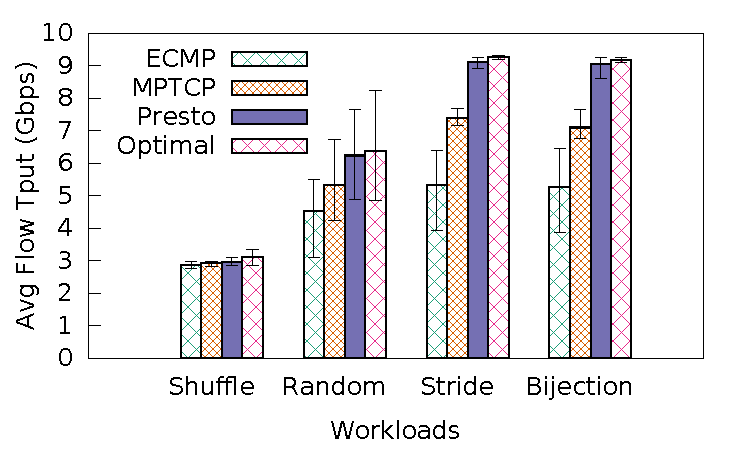
\includegraphics[width=0.55\textwidth]{./figures/presto/macro/stride/macro_compare_tput_witherrbar.pdf}
        \caption{Elephant flow's throughputs of ECMP, MPTCP, Presto and Optimal in Shuffle, Random, Stride and Random Bijection workloads.}
        \label{macro_evaluation_tput}
\end{figure}



\begin{figure*}[!t]
        \centering
	\begin{subfigure}[b]{0.3\textwidth}
                \centering
  		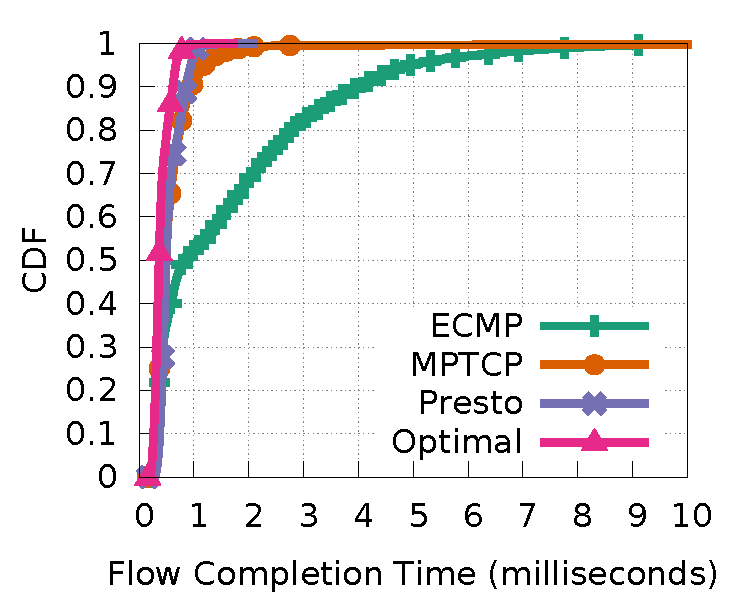
\includegraphics[width=\textwidth]{./figures/presto/macro/stride/macro_compare_fct_stride_mice.pdf}
        	\caption{Stride}
        	\label{macro_evaluation_fct_stride}
	\end{subfigure}
	\begin{subfigure}[b]{0.3\textwidth}
                \centering
		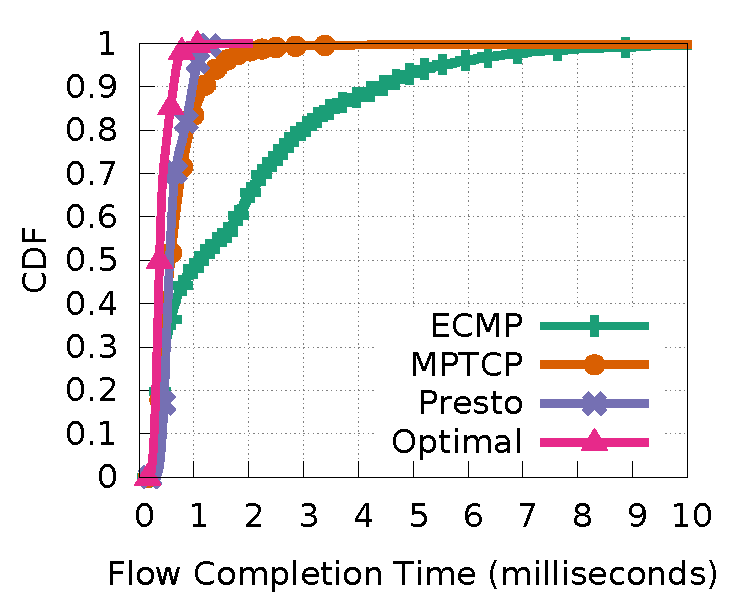
\includegraphics[width=\textwidth]{./figures/presto/macro/bijection/macro_compare_fct_bijection_mice.pdf}
        	\caption{Random Bijection}
        	\label{macro_evaluation_fct_bijection}
	\end{subfigure}
        %\begin{subfigure}[b]{0.225\textwidth}
        %        \centering
	%	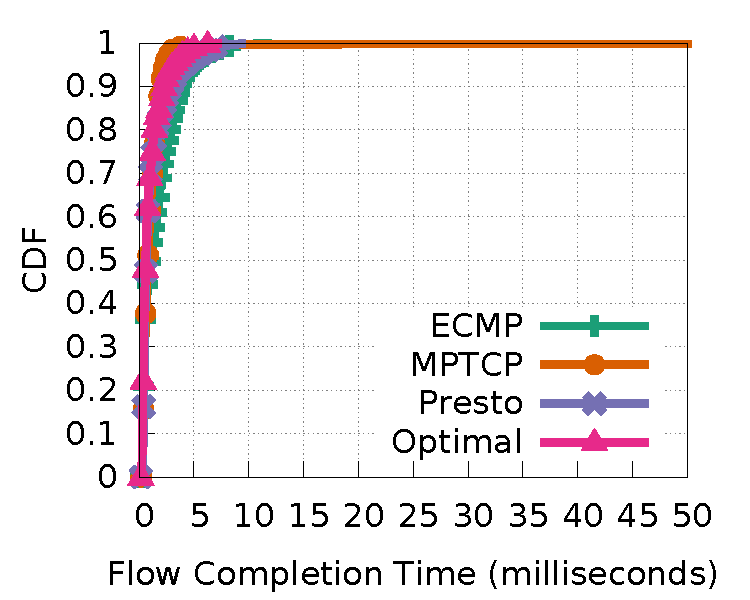
\includegraphics[width=\textwidth]{./figures/macro/random/macro_compare_fct_random_mice.pdf}
        %	\caption{Random}
        %	\label{macro_evaluation_fct_random}
	%\end{subfigure}
        \begin{subfigure}[b]{0.3\textwidth}
                \centering
		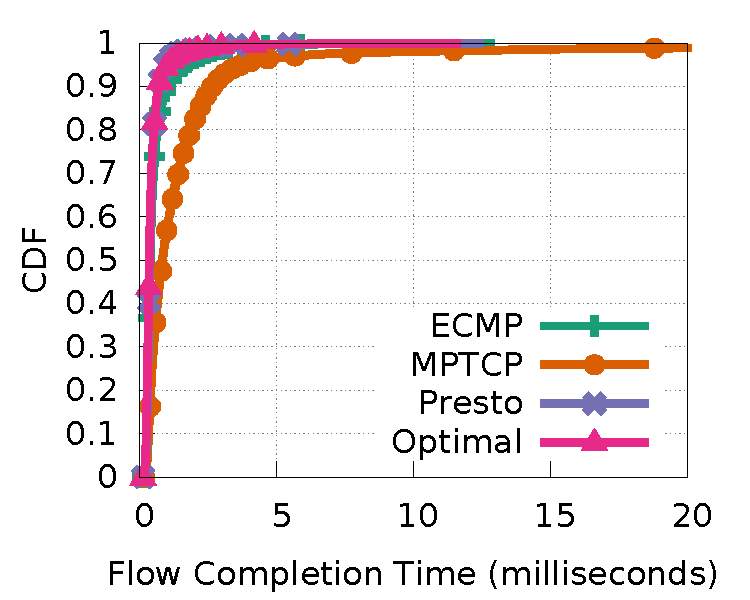
\includegraphics[width=\textwidth]{./figures/presto/macro/shuffle/macro_compare_fct_shuffle_mice.pdf}
        	\caption{Shuffle}
        	\label{macro_evaluation_fct_shuffle}
	\end{subfigure}
	\caption{Mice FCT of ECMP, MPTCP, Presto and Optimal in stride, random bijection, and shuffle workloads.}
	\label{macro_evaluation_fct}
\end{figure*}

\tightparagraph{Synthetic Workloads}
Figure~\ref{macro_evaluation_tput} 
shows the average throughputs of elephant flows in the shuffle, random, stride and random bijection workloads.
Presto's throughput is within 1-4\% of Optimal over all workloads.
For the shuffle workload, ECMP, MPTCP, Presto and Optimal show similar results 
because the throughput is mainly bottlenecked at the receiver. 
In the non-shuffle workloads, Presto improves upon ECMP by 38-72\% and improves
upon MPTCP by 17-28\%.

Figure~\ref{macro_evaluation_fct} shows the mice flow completion time (FCT) in
the workloads. 
The stride and random bijection workloads are non-blocking, and hence the latency of Presto
closely tracks Optimal: the 99.9$^{th}$ percentile FCT for Presto is within 350 $\mu$s for these workloads.
MPTCP and ECMP suffer from congestion, and therefore the tail FCT is much worse than Presto: ECMP's 99.9$^{th}$ percentile
FCT is over 7.5x worse ($\sim$11ms) and MPTCP experiences timeout (because of higher loss
rates and the fact that small sub-flow window sizes from small flows can increase the chances of timeout~\cite{dc-mptcp}).\footnote{We used the Linux default (200ms) and trimmed graphs for clarity}
The difference in the random and shuffle workloads is less pronounced (we omit random due to space constraints).
In these workloads elephant flows can collide on the last hop output port,
and therefore mice FCT is mainly determined by queuing latency. In shuffle, the 99.9$^{th}$ percentile FCT for ECMP, Presto and Optimal
are all within 10\% (MPTCP again experiences TCP timeout) and in random, the 99.9$^{th}$ percentile FCT of Presto is within 25\% of Optimal while ECMP's 
is 32\% worse than Presto.

%%% trace-driven workload, MSR, scaling factor =10
\begin{table}[!tb]
\begin{center}
\begin{tabular}{ |c|c|c|c| }
 \hline
 Percentile & ECMP & Optimal &Presto \\
 \hline
 50\%   & $1.0$ & $-12\%$ & $-9\%$   \\
 90\%   & $1.0$ & $-34\%$ & $-32\%$  \\
 99\%   & $1.0$ & $-63\%$  & $-56\%$ \\
 99.9\% & $1.0$ & $-61\%$ & $-60\%$  \\
 \hline

\end{tabular}
\caption{Mice ($<$100KB) FCT in trace-driven workload~\cite{kandula2009nature}. Negative numbers imply shorter FCT.}
        \label{macro_evaluation_MSR_trace_driven}
\end{center}
\end{table}

\tightparagraph{Trace-driven Workload}
We evaluate Presto using a trace-driven workload based on traffic patterns measured in~\cite{kandula2009nature}. 
Each server establishes a long-lived TCP connection 
with every other server in the testbed. 
Then each server continuously samples flow sizes and inter-arrival times and each time sends to a random receiver
that is not in the same rack.
We scale the flow size distribution by a factor of 10 to emulate a heavier workload. 
Mice flows are defined as flows that are less than 100 KB in size, and elephant flows are defined as flows
that are greater than 1 MB. The mice FCT, normalized to ECMP, 
is shown in Table~\ref{macro_evaluation_MSR_trace_driven}. 
Compared with ECMP, Presto has similar performance at the 50$^{th}$ percentile but reduces the 99$^{th}$ and 99.9$^{th}$ percentile FCT by 56\% and 60\%, respectively. 
Note MPTCP is omitted because its performance was quite unstable in workloads
featuring a large number of small flows.
The average throughput (not shown) for Presto tracks Optimal (within 2\%), and improves upon ECMP by over 10\%.


\begin{table}[!htb]
\begin{center}
\begin{tabular}{ |c|c|c|c|c| }
 \hline

 Percentile & ECMP & Optimal & Presto & MPTCP \\
 \hline
 50\%       & 1.0 & $-34$\%     & $-20$\%   & $-12$\% \\
 90\%       & 1.0 & $-83$\%     & $-79$\%   & $-73$\% \\
 99\%       & 1.0 & $-89$\%     & $-86$\%   & $-73$\% \\
 99.9\%     & 1.0 & $-91$\%      & $-87$\%   & TIMEOUT \\

 \hline
\end{tabular}
\caption{FCT comparison (normalized to ECMP) with ECMP load balanced north-south traffic.}
	\label{macro_evaluation_north_south_traffic}
\end{center}
\end{table}


\tightparagraph{Impact of North-South Cross Traffic}
Presto load balances on ``east-west'' traffic in the datacenter, \ie{}, traffic
originating and ending at servers in the datacenter. 
In a real datacenter environment "north-south" traffic (\ie{}, traffic with an endpoint outside the datacenter)
must also be considered. 
To study the impact of north-south traffic on Presto, we attach an additional server to 
each spine switch in our testbed to emulate remote users. 
The 16 servers establish a long-lived TCP connection with each remote user. 
Next, each server starts a flow to a random remote user every 1 millisecond. This emulates  
the behavior of using ECMP to load balance north-south traffic.
The flow sizes for north-south traffic are based on the distribution measurement in~\cite{he2013next}. 
The throughput to remote users is limited to 100Mbps to emulate the limitation of an Internet WAN. 
Along with the north-south flows, 
a stride workload is started to emulate the east-west traffic. 
The east-west mice FCT is shown in Table~\ref{macro_evaluation_north_south_traffic} (normalized to ECMP). 
ECMP, MPTCP, Presto, and Optimal's average throughput is 
5.7, 7.4, 8.2, and 8.9Gbps respectively. 
The experiment shows Presto can gracefully co-exist with north-south cross traffic
in the datacenter.


%%%failure handling experiments

\begin{figure}[t]
        \centering
  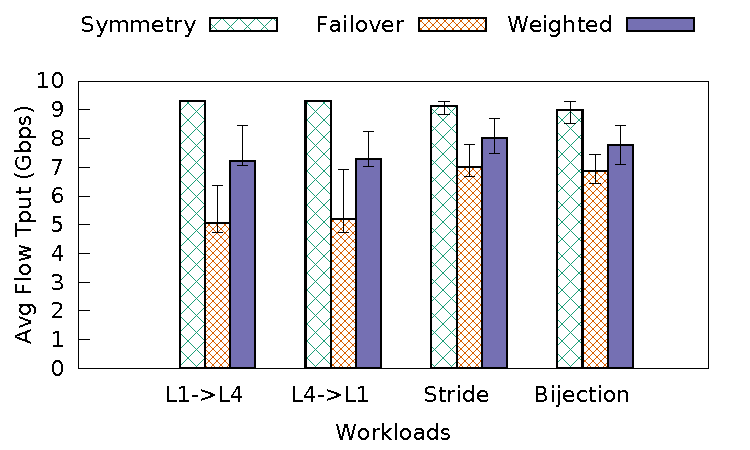
\includegraphics[width=0.55\textwidth]{./figures/presto/failure_handling/failover_compare_tput_witherrbar.pdf}
        \caption{Presto's throughput in symmetry, fast failover and weighted multipathing stages for different workloads.}
        \label{failover_compare_tput}
\end{figure}

\begin{figure}[t]
        \centering
  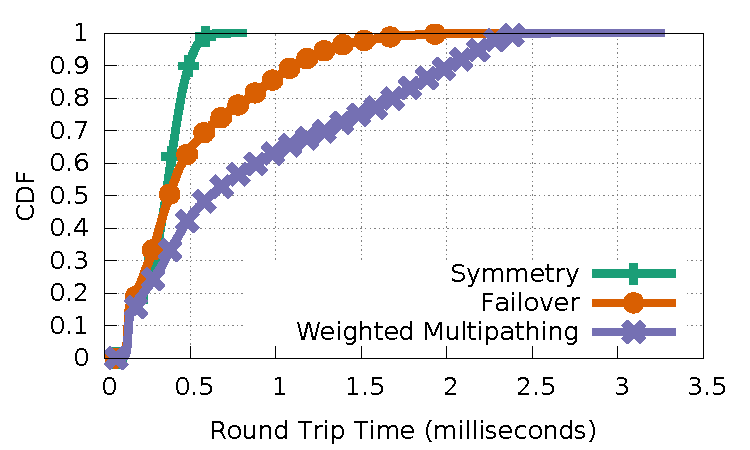
\includegraphics[width=0.55\textwidth]{./figures/presto/failure_handling/failover_compare_sockperf_bijection_mice.pdf}
        \caption{Presto's RTT in symmetry, fast failover and weighted multipathing stages in  random bijection workload.}
        \label{failover_compare_sockperf_bijection}
\end{figure}

\tightparagraph{Impact of Link Failure}
Finally, we study the impact of link failure.
Figure~\ref{failover_compare_tput} compares the throughputs of
Presto when %under different stages of loss recovery when 
the link between spine switch S1 and leaf switch L1 goes down.
Three stages are defined: symmetry (the link is up), failover (hardware fast-failover moves traffic from S1 to S2), and weighted (the controller
learns of the failure and prunes the tree with the bad link).
Despite the asymmetry in the topology, Presto still achieves reasonable average throughput at 
each stage.
Figure~\ref{failover_compare_sockperf_bijection} shows the round trip time of
each stage in a random bijection workload. 
Workload L1$\rightarrow$L4 is when each node connected to L1 sends to one node in L4 
(L4$\rightarrow$L1 is the opposite).
Due to the fact that the network is no longer non-blocking after the link failure,
failover and weighted multipathing stages have larger round trip time.

%\subsection{Conclusion}
\label{sec:presto-conclusion}
Presto is a near uniform sub-flow distributed load balancing scheme
that can near optimally load balance the network at fast networking speeds.
Our scheme makes a few simple changes to the hypervisor soft-edge (vSwitch and GRO)
and does not require any modifications to the transport layer or network hardware, making
the bar for deployment lower. 
Presto is explicitly designed to load balance the network at fine granularities
and deal with reordering without imposing too much overhead on hosts. Presto is flexible and can also
deal with failures and asymmetry. Finally, we show the performance of Presto can closely track
that of an optimal non-blocking switch, meaning elephant throughputs remain high while the tail
latencies of mice flow completion times do not grow due to congestion.


%\section{Latency in Software Defined Networks: Measurements and Mitigation Techniques}
\label{mazu}


Timely interaction between an SDN controller and switches is crucial to many
SDN applications---e.g., fast rerouting during link failure and fine-grained
traffic engineering in data centers. However, it is not well understood how
the control plane in SDN switches impacts these applications. To this end, we
conduct a comprehensive measurement study using four
types of production SDN switches. Our measurements show that control actions,
such as rule installation, have surprisingly high latency, due to both
software implementation inefficiencies and fundamental traits of switch
hardware.

Based on our measurements, we propose three techniques to mitigate the outbound latencies
imposed by current switches:
{\em Flow engineering} (FE) leverages our empirical latency models to compute
paths such that the latency of installing forwarding state at any
switch is minimized.
{\em Rule
  offloading} (RO) computes strategies for opportunistically
offloading installation of some forwarding state to downstream switches.
Finally, {\em rule reordering} (RR) sends rule installation
requests in an order that is optimal for the switch in question. By reducing
installation latency per switch (FE + RR) and enabling network-wide parallel
updates (RO),
rule updates can finish much faster.

\subsection{The Control Plane Latency in SDN}
\label{mazu-background}

Instead of running a complex control plane on each switch, SDN delegates
network control to external applications running on a logically central
controller. 
Applications determine the routes traffic should take, and they
instruct the controller to update switches with the appropriate forwarding
state. These decisions may be based on data packets that are
received by switches and sent to the controller. Such packet events and
state update operations are enabled by OpenFlow~\cite{openflow}---a standard
API implemented by switches to facilitate communication with the controller.
Although SDN moves control plane logic from switches to a central controller, 
switches must still perform several steps to generate packet events and update
forwarding state. We describe these steps below.

\begin{figure}
\centering
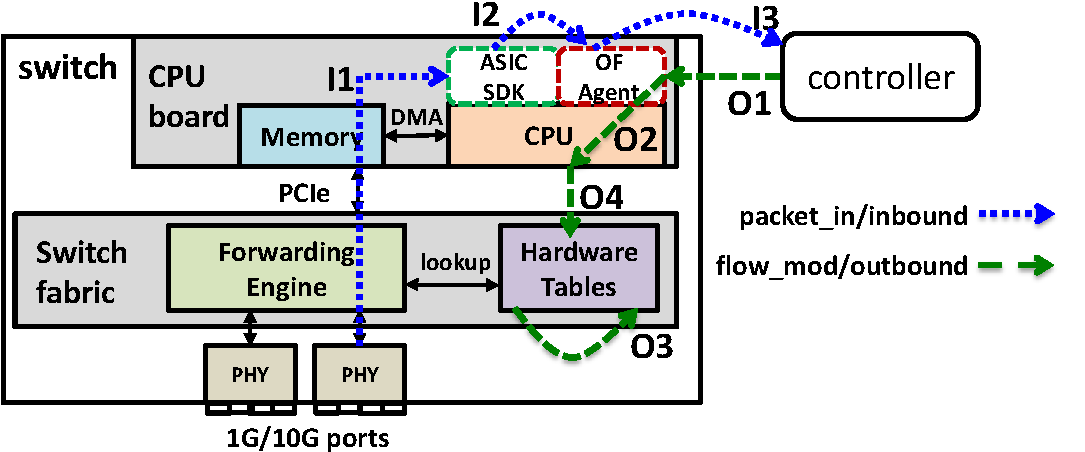
\includegraphics[width=0.55\textwidth]{figures/mazu/openflow_switch.pdf}
\caption{Schematic of an OpenFlow switch. 
We also show the factors contributing to inbound and outbound latency}\label{openflow_switch_delay}
\end{figure}

\tightparagraph{Packet Arrival} When a packet arrives, the switch ASIC first
performs a lookup in the switch's hardware forwarding tables. If a match is
found, the packet is forwarded at line rate. Otherwise the following steps
occur (Figure~\ref{openflow_switch_delay}): (I1) The ASIC sends the packet to the switch's CPU via the PCIe bus. (I2) An OS
interrupt is raised, at which point the ASIC SDK gets the packet and
dispatches it to the switch-side OpenFlow agent. (I3) The agent wakes up,
processes the packet, and sends to the controller a \packetin message
containing metadata and the first 128B of the packet. All three steps,
I1--I3, can impact the latency in generating a \packetin message. We
categorize this as {\em inbound latency}, since the controller receives the
message as input.

\tightparagraph{Forwarding Table Updates} 
The controller sends \flowmod messages to update a
switch's forwarding tables.
A switch takes the following steps to handle a \flowmod
(Figure~\ref{openflow_switch_delay}): (O1) The
OpenFlow agent running on the CPU parses the message. (O2) The agent
schedules the addition (or removal) of the forwarding rule in hardware tables, typically TCAM.  (O3)
Depending on the nature of the rule, the chip SDK may require existing rules
in the tables to be rearranged, e.g., to accommodate high priority rules.
(O4) The rule is inserted (or removed) in the hardware table.  All four steps, O1--O4,
impact the total latency in executing a \flowmod action. We categorize this
as {\em outbound latency}, since the controller outputs a \flowmod message.

\subsection{Motivating Applications}
\label{mazu-motivation-apps}

We now provide examples of management
applications that require fine-grained control over data plane state and
discuss why the control plane latency problem in SDN-enabled switches impacts
such applications. 

\tightparagraph{Failover}
It is possible that SDN can help mitigate the network-wide impact of
failures in wide-area networks, reducing both downtime and congestion
without requiring significant over provisioning. When failures occur,
the SDN management application can quickly compute new paths for flows
traversing failed nodes or links, while also simultaneously rerouting
other high/low priority flows so as to avoid hot-spots~\cite{hong2013achieving}.
However, this requires significant updates to network state at
multiple network switches. The longer these updates take, the longer
the effect of failure is felt in the form of congestion and drops. We
find that outbound latencies can inflate the time by nearly 20s
(\secref{mazu-evaluation}) putting into question SDN's applicability to
this scenario. 

\tightparagraph{Intra-Datacenter Traffic Engineering} 
Micro\-TE~\cite{benson2011microte}, Hedera~\cite{al2010hedera}, 
and other recent proposals have
argued for using SDN to route traffic subsets at fine time-scales in order to
achieve fine-grained traffic engineering in data centers. For instance,
MicroTE leverages the fact that a significant fraction of ToR-to-ToR DC
traffic (ToR is ``top-of-rack'' switch) is predictable on short time-scales
of 1-2s. It computes and installs at ToR switches routes for such traffic
on short time-scales. % The computed routes may only be effective for 1-2s
% after which a new sets of routes may be more optimal. 
Thus, latencies in installing routes can significantly undermine MicroTE's
effectiveness. Indeed, we find that updating a set of routes at a ToR switch
in MicroTE can take as long as 0.5s on some SDN switches
(\secref{mazu-evaluation}). 

\subsection{Latency Measurements}
\label{mazu-measure}

In this section, we systematically measure in/outbound latencies to
understand what factors contribute to high latencies. We generate a variety
of workloads to isolate specific factors, and we use production switches from
\numVendors vendors, running switch software with support for OpenFlow
1.0~\cite{openflow} or, if available, OpenFlow 1.3, to highlight the
generality of our observations and to understand how software evolution
impacts latencies.\footnote{When using OpenFlow 1.3 firmware, we
only leverage features also available in OpenFlow 1.0 for an apples-to-apples comparison.} 
Henceforth, we refer to the \numCombos hardware and software combinations
(\tabref{switch_para}) as \Intel, \BroadcomOne, \BroadcomThree, and \IBM.
To ensure we are experimenting in the optimal regimes for each switch, we take
into account factors such as flow table capacity and support for \packetin.

\begin{table}
\centering
\small
\begin{tabular}{|l|c|c|c|c|c|}
\hline
\bf Model & \bf CPU & \bf RAM & \tabincell{c}{\bf OF\\\bf Ver.} 
    & \tabincell{c}{\bf Flow\\\bf Table Size} & \bf Ifaces\\ 
\hline
\tabincell{l}{Intel\\FM6000} &  2Ghz & 2GB & 1.0 & 4096 
    & \tabincell{c}{40x10G\\+ 4x40G} \\ 
\hline
\multirow{2}{*}{\tabincell{l}{Broadcom \\956846K}} & \multirow{2}{*}{1Ghz} 
    & \multirow{2}{*}{1GB} & 1.0 & 896 
    & \multirow{2}{*}{\tabincell{c}{14x10G\\+ 4x40G}}\\ 
\cline{4-5}
& & & 1.3 & 1792 (ACL tbl) & \\
\hline
\tabincell{l}{IBM\\G8264} &  ? & ? & 1.0 & 750
    & \tabincell{c}{48x10G \\+ 4x40G} \\ 
\hline
\end{tabular}
\caption{Switch specifications}{\label{switch_para}}
\end{table}


\subsubsection{Measurement Methodology}

\begin{figure}[!tb]
\centering

\includegraphics[width=0.55\textwidth]{figures/mazu/experiment_setup.pdf}
\caption{Measurement experiment setup}
\label{mazu_experiment_setup} 
\end{figure}

\figref{mazu_experiment_setup} shows our measurement setup.
The host has one 1Gbps and two 10Gbps interfaces connected to the switch under test. 
The eth0 interface is connected to the control port of the switch, and an SDN
controller (POX for \Intel, \BroadcomOne, and \IBM; RYU for \BroadcomThree) running
on the host listens on this interface. 
The RTT between switch and controller is
negligible ($\approx$0.1ms). We use the controller to send a burst of OpenFlow 
\flowmod commands to the switch. For \Intel, \BroadcomOne, and \IBM, we
install/modify/delete rules in the single table supported by OpenFlow 1.0;
for \BroadcomThree, we use the highest numbered table, which supports
rules defined over any L2, L3, or L4 header fields.
The host's eth1 and eth2 interfaces are connected to data ports on the
switch. We run pktgen~\cite{pktgen} in kernel space to generate traffic on
eth1 at a rate of 600-1000Mbps using minimum Ethernet frame size.

Prior work notes that accurate execution times for OpenFlow commands on
commercial switches can only be observed in the data plane~\cite{rotsos2012oflops}.
Thus, we craft our experiments to ensure the latency impact of various
factors can be measured directly from the data plane (at eth2 in
\figref{mazu_experiment_setup}), with the exception of \packetin generation
latency. We run \emph{libpcap} on our measurement host to accurately
timestamp the packet and rule processing events of each flow. We first log
the timestamps in memory, and when the experimental run is complete, the
results are dumped to disk and processed. We use the timestamp of the
first packet associated with a particular flow as the finish time of the
corresponding \flowmod command; more details are provided later in this
section.

\subsubsection{Dissecting Inbound Latency}
\label{mazu-measure_inbound}

\begin{figure*}
	\centering
	\begin{subfigure}[b]{0.40\textwidth}
	\centering
	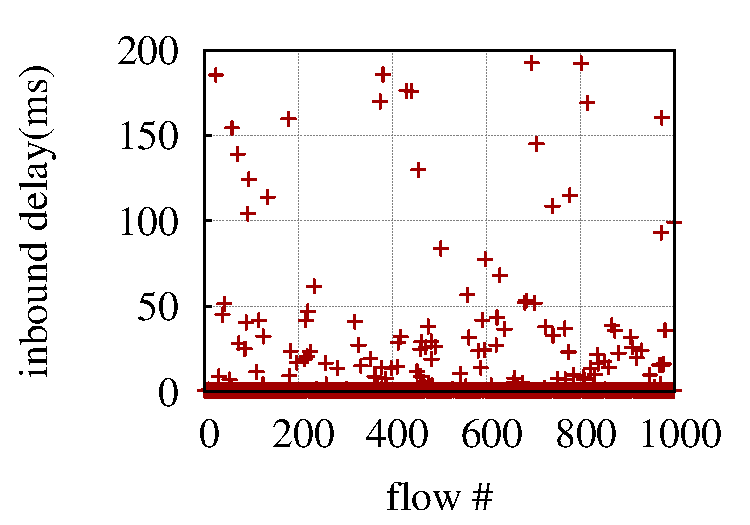
\includegraphics[width=\textwidth]{./figures/mazu/jan27_intel_inbound_with_pktout_flowmod_rate200-eps-converted-to.pdf}
	\caption{with flow\_mod/pkt\_out}
	\label{fig:intel_inbound_test3}
	\end{subfigure}
	\centering
        \begin{subfigure}[b]{0.40\textwidth}
        \centering
	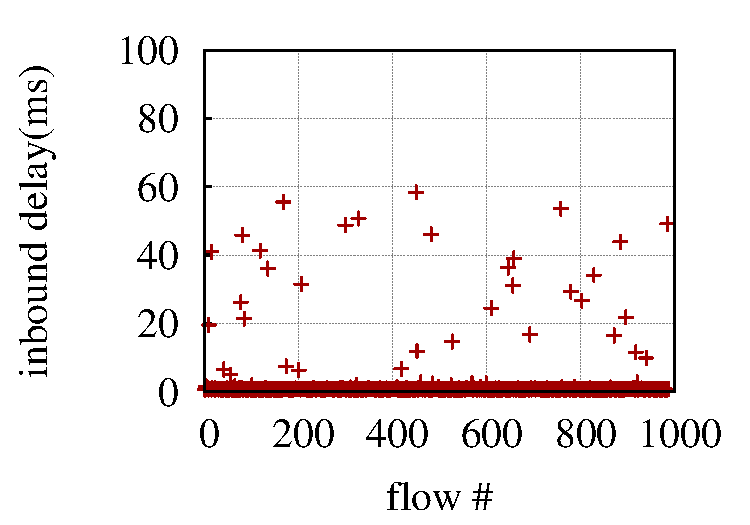
\includegraphics[width=\textwidth]{./figures/mazu/jan27_intel_inbound_wo_pktout_flowmod-eps-converted-to.pdf}
	\caption{w/o flow\_mod/pkt\_out}
	\label{fig:intel_inbound_test3_wo}
	\end{subfigure}	
	\caption{{\bf Inbound delay} on {\bf \Intel}, flow arrival rate = 200/s} 
	\label{fig:inbound-1}
\end{figure*}

To measure inbound latency, we empty the table at the switch, and we generate
traffic such that \packetin events are generated at a certain rate (i.e., we
create packets for new flows at a fixed rate). To isolate the impact of
\packetin processing from other message processing, we perform two kinds of
experiments: (1) the \packetin will trigger corresponding \flowmod (insert
simple OpenFlow rules differing just in destination IP) and \packetout
messages; (2) the\linebreak \packetin message is dropped silently by the
controller. 

We record the timestamp ($t_1$) when each packet is transmitted on the
measurement host's eth1 interface (\figref{mazu_experiment_setup}). We also record
the timestamp ($t_2$) when the host receives the corresponding \packetin
message on eth0. The difference ($t_2 - t_1$) is the inbound
latency.\footnote{Our technique differs from \cite{huang2013high}, where the
delay was captured from the switch to the controller, which includes
controller overhead.}


\begin{table}
\centering
\begin{scriptsize}
\begin{tabular}{cc}
\begin{tabular}{|c|c|c|}
\hline
\multicolumn{3}{|c|}{with flow mod/pkt out} \\ \hline
flow rate & 100/s  & 200/s  \\ \hline
cpu usage & 15.7\%    & 26.5\%   \\ \hline
\end{tabular}
&
\begin{tabular}{|c|c|c|}
\hline
\multicolumn{3}{|c|}{w/o flow mod/pkt out} \\ \hline
flow rate & 100/s   & 200/s \\ \hline
cpu usage & 9.8\%     & 14.4\%   \\ \hline
\end{tabular}
\end{tabular}
\caption{CPU usage on \Intel}
\label{fig:inbound-cpu}
\end{scriptsize}
\end{table} 

Representative results for an \Intel switch are shown in
\figref{fig:inbound-1};
\IBM has similar performance (5ms latency per \packetin on 
average).\footnote{\BroadcomOne and \BroadcomThree do not support \packetin
messages.} In the first experiment (\figref{fig:intel_inbound_test3}), we see the inbound latency is quite
variable with a mean of 8.33ms, a median of 0.73ms, and a standard deviation
of 31.34ms. In the second experiment (\figref{fig:intel_inbound_test3_wo}), the inbound delay is lower (mean of 
1.72ms, median of 0.67ms) and less variable (standard deviation of 6.09ms). 
We also observe that inbound latency depends on the \packetin rate: e.g. in
the first experiment the mean is 3.32 ms for 100 flows/s (not shown) vs. 8.33ms
for 200 flows/s (\figref{fig:intel_inbound_test3}).

The only difference between the two experiments is that in the former case
the switch CPU must process \flowmod and \packetout messages, and send
forwarding entries and outbound packets across the PCIe bus to the ASIC, in
addition to generating \packetin messages. As such, we observe that the CPU
usage is higher when the switch is handling concurrent OpenFlow operations and
generating more \packetin messages (\tabref{fig:inbound-cpu}). However, since
the Intel switch features a powerful CPU (\tabref{switch_para}), plenty of
CPU capacity remains. Our conversations with the switch vendor suggest that
the limited bus bandwidth between the ASIC and switch CPU is the primary
factor contributing to inbound latency. 

 

\subsubsection{Dissecting Outbound Delay} 
\label{mazu-outbound_meas}

We now study the outbound latencies for three different \flowmod\
operations: insertion, modification, and deletion. For each operation, we
examine the latency impact of key factors, including table
occupancy and rule priority.
Before measuring outbound latency, we install a single default low priority
rule which instructs the switch to drop all traffic. We then install a set of
non-overlapping OpenFlow rules that
eth2 interface of our measurement host. For some experiments, we 
systematically vary the rule priorities.

\input{mazu_measure_flowmod_insert}
\input{mazu_measure_flowmod_modify}
\input{mazu_measure_flowmod_delete}

\subsection{Implications}


A subset of our findings highlight 
problems with the firm\-ware on OpenFlow switches:
e.g., rule insertion latencies are 3ms with \BroadcomOne, which is significantly higher than the 
update rate that TCAM hardware natively supports~\cite{estan:private}. 
We believe near term work will reduce such issues, as indicated by
improved latencies in \BroadcomThree. 
However, given that software will continue to bridge 
control and data planes in SDN switches, we remain skeptical whether 
latencies will ever reach what hardware can natively support.


Our measurements also reveal root causes of latency that appear to be
fundamentally entrenched in hardware design: e.g., rules 
must be organized in the TCAM in a priority order for correct and efficient matching; 
also, \packetin, \flowmod, and \packetout messages must contend for limited
bus bandwidth between a switch's CPU and ASIC. Unless the hardware
significantly changes, we believe the latencies we identify
will continue to manifest in next generation switches.  



\subsection{Mitigating the Latency of Programming Network State}

\subsubsection{Flow Engineering}
\label{mazu-floweng}

\begin{figure}
\centering
  \centering
  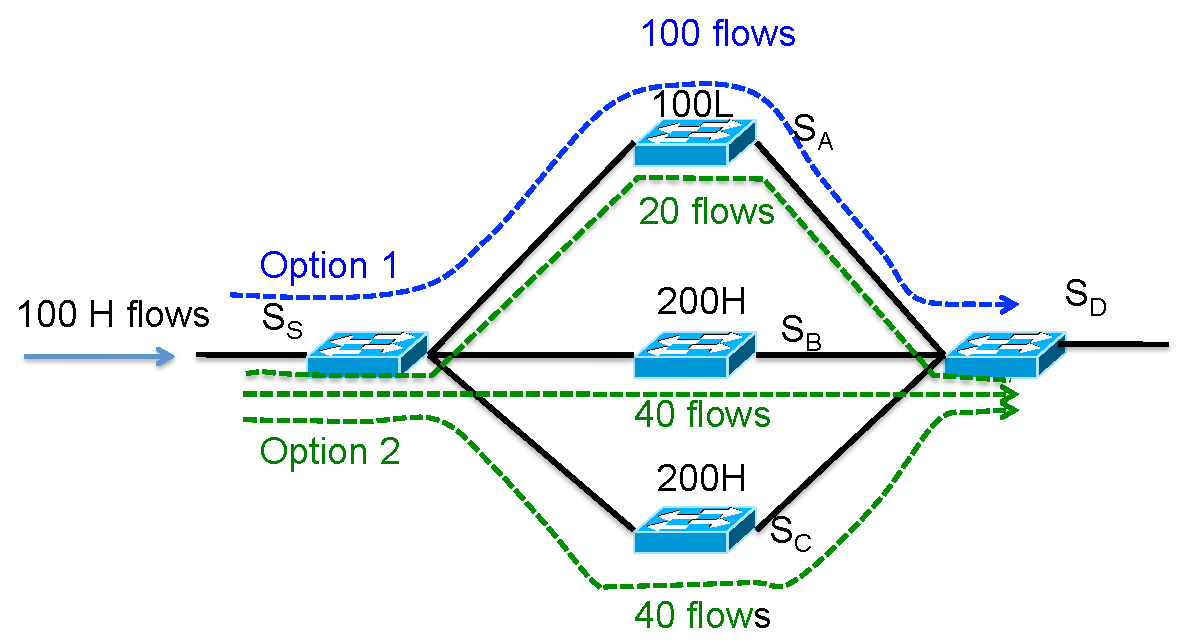
\includegraphics[width=0.55\textwidth]{figures/mazu/flow_eng_example.pdf} 
\caption{Flow 
engineering example, assuming \BroadcomOne. $nL$ = $n$ low priority rules;
$nH$ = $n$ high priority rules; capacity = 1000 rules. Ingress and egress 
tables are empty} 
\label{fig:flow_eng} 
\end{figure}

SDN applications that perform failure recovery, traffic engineering, or other
forms of routing must quickly compute and setup network paths in order to
satisfy reachability and performance objectives. These applications must often
select one of many possible paths based on congestion, delay, flow table 
occupancy, or other metrics. Unfortunately, a (slightly) more optimal path 
according to these metrics may take significantly longer to setup due to 
outbound latency.

For example, consider an SDN application that seeks to minimize the
imbalance in flow table occupancy~\cite{hong2013achieving, qazi2013simple, moshref2013vcrib}. If such an
application needed to setup routes for 100 flows of high priority $H$ in the
topology shown in Figure~\ref{fig:flow_eng}, it would select the first path
through switch $S_A$ for all flows, thereby equalizing the number of flow
table entries across all switches. However, assuming the switches are
\BroadcomOne, this would require displacing {\em each} of the 100 existing
rules of low priority $L$ in $S_A$ for {\em each} of the 100 new flows,
resulting in a total flow installation time of $\approx$1.5s. In contrast, by
routing only 20 new flows through $S_A$, and dividing the remaining flows
evenly between the paths through $S_B$ and $S_C$, we can keep the same level
of imbalance in flow table occupancy ($S_B$ and $S_C$ each have twice as many
entries as $S_A$), while reducing the total flow installation time to
$\approx$0.3s (assuming rules are installed in $S_A$, $S_B$, and $S_C$ in
parallel). 


The goal of {\em flow engineering} (\FE) is to select paths that minimize
installation delay while still satisfying an SDN application's primary path
selection criteria (e.g., flow table occupancy or congestion). Assuming there
are many possible sets of paths $\{\mathcal{P}^i_{obj}\}_i$ that (closely)
satisfy an application's objectives, FE selects the set
$\mathcal{P}^{displace}_{obj,tbl\_sz}$ that minimizes the aggregate
latency impact of rule installations, and any associated rule displacements,
while still obeying flow table space constraints.
$\mathcal{P}^{displace}_{obj,tbl\_sz}$ can be computed using a two step
optimization:
({\em i}) identify sets of paths that satisfy the SDN application's objective 
function,
but do not select the actual
paths to use; ({\em ii}) select paths that minimize aggregate
flow installation time.
Unfortunately, the time required to solve the integer linear program would
outweigh the latency benefits it seeks provide, so we formulate an
efficient heuristic.

\tightparagraph{Flow Engineering Heuristic}
Our goal is to satisfy a bound $C$ on the time required to install/modify
rules across all switches. 

We represent the network as a graph $G = (V,E)$, where each node is a switch
(or PoP) and each edge is a link (or tunnel). Given a traffic matrix $M$, the
SDN application computes $K$ candidate equal cost paths for each $(u,v) \in
V$, where cost is defined in terms of the application's objective (e.g.,
average link utilization). We assume the application also assigns a priority
$Pri(u,v)$ to each flow $(u,v)$.


We sort the flows in decreasing order of resource demand (e.g., bandwidth) and
iterate through them. For each flow $(u,v)$ in the sorted order, we consider
the corresponding $K$ equal cost paths in decreasing order of resource 
availability; let $P^{1\ldots K}_{(u,v)}$ be the sorted order. If the resource
demand $d_{uv}$ can be satisfied by the path $P^{1}_{(u,v)}$, then we compute
whether installing/updating rules for flow $(u,v)$ along this path violates the
latency bound $C$.

Given our measurement results, for every switch $s \in P^{1}_{(u,v)}$, we can
model the latency at $s$ due to installing rules for $(u,v)$ as 
$L_s = \max(a, (b +c * Disp_s(Pri(u,v))))$. Here, $Disp_s(Pri(u,v))$ is the 
number of rules at $s$ that will be displaced by the rule for $(u,v)$.
$a$, $b$ and $c$ are constants derived from switch
measurements. This model essentially says that if the current rule
does not displace any rules from $s$'s existing table, then it incurs
a fixed cost of $a$; otherwise, it incurs the cost given by $b +c *
Disp_s(Pri(u,v))$. The fixed cost $a$ is the insertion delay without any TCAM
reordering. 

Now, $\forall s \in P^{1}_{(u,v)}$, we check if $L_s + CurrentL_s \le C$,
where $CurrentL_s$ is the current running total cost of installing the
rules at $s$, accumulated from vertex pairs considered prior to $(u,v)$ in our
iterative approach.
If this inequality is satisfied, we assign $(u,v)$ to the path
$P^{1}_{(u,v)}$ and move to the next vertex pair. If not,
we move to the next candidate path for $(u,v)$, i.e., $P^{2}_{(u,v)}$ and
repeat the process.
If after iterating through all flows once, we have not selected a feasible
path for each flow, then we increase $C$ and start from the beginning.
Alternately, we could do a simple binary search on $C$. 

\tightparagraph{Limitations} Because paths are computed by the SDN application, FE
must be integrated with the application. FE does not apply to scenarios where 
route updates are confined to a single location, presenting no opportunity to
spread update load laterally. One such example is MicroTE~\cite{benson2011microte},
where changes in traffic demands are accommodated by altering rules at the
source ToR to reallocate ToR-to-ToR flows across different tunnels.


\subsubsection{Rule Offload}
\label{mazu-offload}

\begin{figure}
\centering
  \centering
  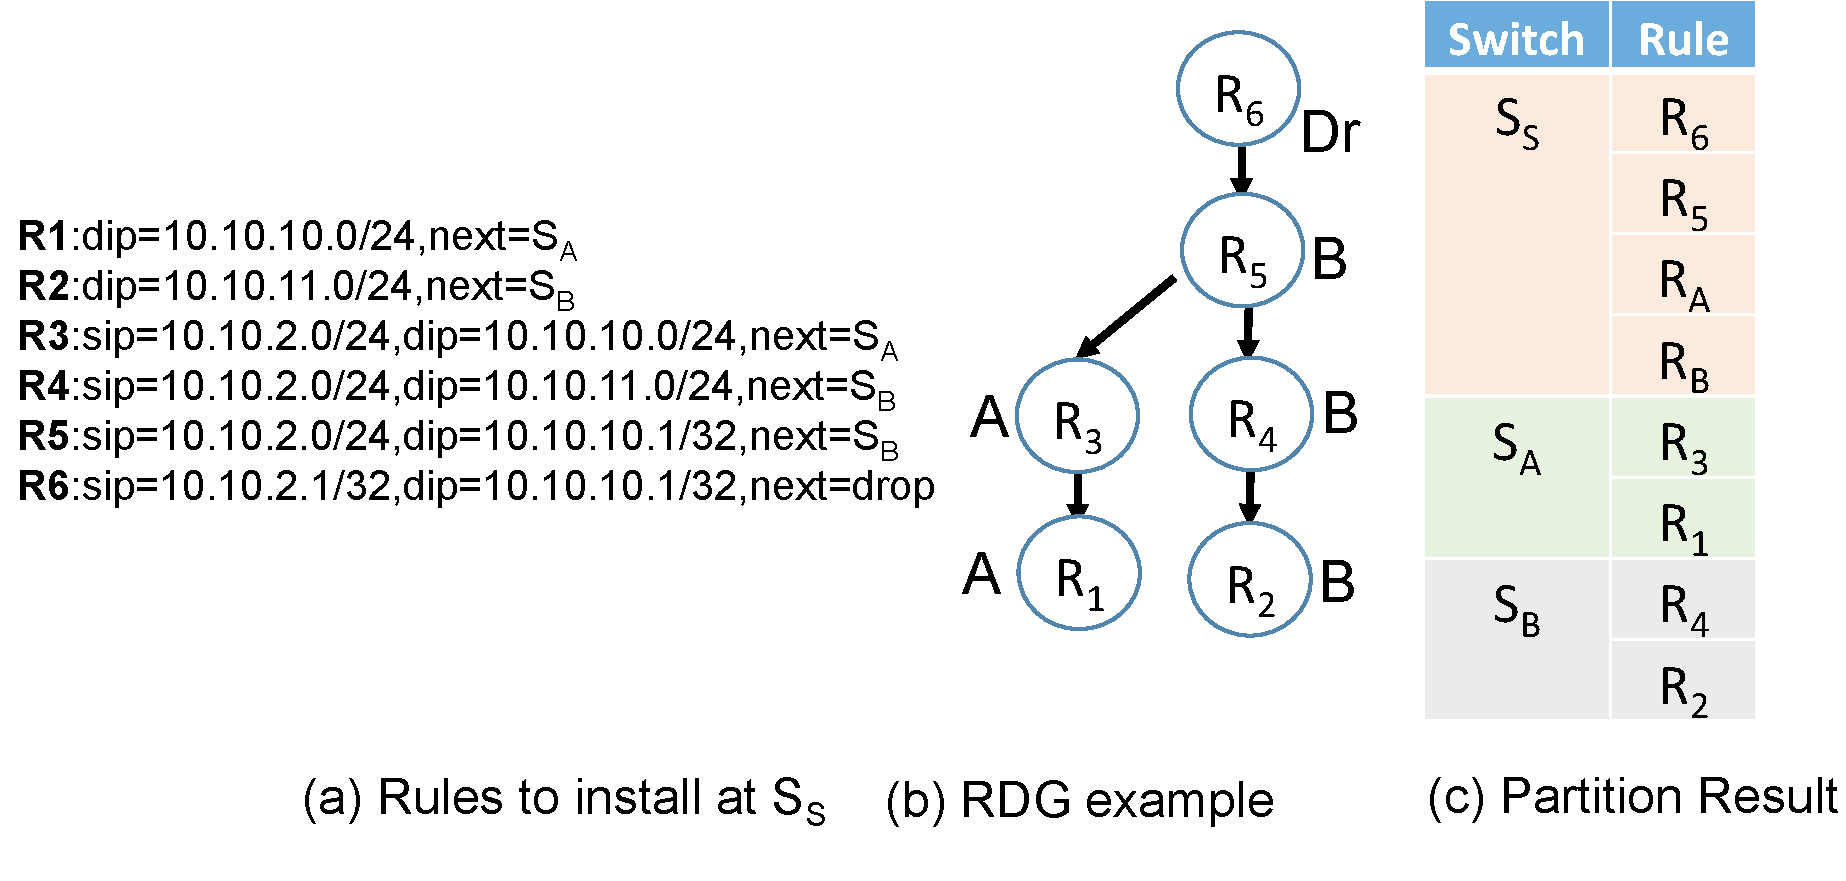
\includegraphics[width=0.55\textwidth]{figures/mazu/Rule-Offload2.pdf}
\caption{Rule offloading example}
\label{fig:rule-offload}
\end{figure}

When FE selects a path for a set of flows, the same number of rules are
installed/modified in every switch along the path. Thus, a path's update
latency is determined by the switch with the largest number of existing
low priority rules (assuming \BroadcomOne), or the largest number of pending
rule installations/modifications. For example, since switch $S_S$ in
\figref{fig:flow_eng} is part of all three paths to reach switch $S_D$, a
rule must be installed in $S_S$ for every new flow, regardless of whether the
flow traverses the path through $S_A$, $S_B$, or $S_C$.  Assuming
\BroadcomOne switches, it will take at least 0.3s to install rules for 100
flows of high priority $H$ in $S_S$---the same time required to install 20
rules in $S_A$ and longer than the $\approx$0.12s required to install 40
rules in both $S_B$ and $S_C$.

The goal of {\em rule offloading} (\RO) is to partition rules into subsets
that can be installed at downstream switches, with the appropriate {\em
default rules} installed at upstream switches. If the original number of
rules is $N$ and no partition (together with default rules) has more than $H$
rules, then, by updating the partitions in parallel, we can reduce rule
installation latency by a factor of $\frac{N}{H}$. 

Our algorithm consists of two phases. First, given a set of rules slated for
installation in a switch $S$ (called the {\em root} switch), we partition the
rules based on their next hop, taking into account any overlap between
rules. Second, we compute default rules for each partition; these rules are
installed in the root switch to direct packets to the next hop switch where
the original rules are actually installed.

\tightparagraph{Rule Partitioning Algorithm}
We represent the rules to be installed at a switch as a rule dependency graph
(RDG). In an RDG, a node denotes a rule, an edge represents a dependency
between two rules, and a node label indicates a rule's action (or next hop
switch). For example, \figref{fig:rule-offload}(b) depicts the RDG for the
six rules in \figref{fig:rule-offload}(a), which are slated for installation
in switch $S_S$ in the topology in \figref{fig:flow_eng}.  Note that when
rules send packets over a tunnel, we specify the next hop in the tunnel path,
not the tunnel destination, as the node label.

%\input{algs/partition}

The algorithm performs a reverse breadth-first
traversal of the RDG. If a node $R$ is a leaf node, then it is eligible to be
placed in partition $P_i$, where $i$ is $R$'s label (or next hop). A leaf
node $R$ is placed in $P_i$ if the current number of rules in $P_i$ is less
than $H_{down}$, otherwise $R$ is placed in $P_{root}$. $H_{down}$ controls 
the maximum number of rules we can offload to a switch downstream from the root switch. If a node $R$ is not
a leaf node, then it is only placed in partition $P_i$ if all of its children
are also in partition $P_i$, and the current number of rules in $P_i$ is less
than $H_{down}$. Otherwise, $R$ is placed in $P_{root}$.
The result is an allocation of rules $R \in RDG$ to the root switch ($S$) and
its next hops.
In the example (\figref{fig:rule-offload}), $R_1$ and $R_3$ are assigned to
partition $P_A$, $R_2$ and $R_4$ are assigned to $P_B$, and $R_5$ and $R_6$
are assigned to $P_{root}$. 
   

\tightparagraph{Computing Default Rules} 
Given the partitions for the next hop switches, we must compute a set of
default rules that {\em cover} the rules in each partition. These default
rules are added to $P_{root}$ to forward packets to the appropriate next hop
switch, where the rules in each partition (excluding $P_{root}$) are 
installed.
The main challenge is dealing with the fact that the intersection of default
rules may include rules from multiple partitions. 
Splitting the default rules into smaller rules can address this, but we must
be careful not to introduce too may default rules and undo the benefits of
RO.

Our heuristic from computing default rules is discussed below. Given the rules in a pair of partitions $P_i$ and
$P_j$, we create a {\em covering rectangle} for the rules in each partition,
denoted as $C_i$ and $C_j$. A covering rectangle is one whose source IP range
covers the entire source IP range specified in the rules in a partition;
likewise for destination IPs. This can easily be extended to higher
dimensions if rules are based on more than just source and destination IPs.

If the number of rules from either $P_i$ or $P_j$ in $C_i \cap C_j$ is below
a threshold $\Theta$, then all such rules are ``promoted'' to the root
partition $P_{root}$. We also create two default rules, one each for
$C_i$ and $C_j$, and install them in the root switch $S$.

If, however, the number of rules in $C_i \cap C_j$ exceeds $\Theta$, then we
further divide both $C_i$ and $C_j$ into two sub-rectangles, and we repeat
the process above for pairs of sub-rectangles, one from each partition.
We recursively repeat the process for a small number of steps. If at the
end of these steps, the combined number of default rules and rules in
$P_{root}$ is significant ($> \Omega$), then we merge $P_i$ and $P_j$ and
simply install all of their rules at the root switch $S$.

%\input{algs/default_rule}

We recursively apply RO to the switches in a set of paths, starting at the
ingress switch for the paths (e.g., $S_S$ in \figref{fig:flow_eng}),
followed by the second switch in each path, and so on.
The termination condition is that a set number of hops in each path are
explored. If at termination, the number of rules accommodated at every
switch, except the ingress switch, is $<H$, then we lower $H$ by a factor
$\gamma < 1$ and repeat again. If $H^*$ is the value of $H$ at the last of
such iterations, then we achieve a speedup of $\frac{N}{H^*}$ from installing
the offloaded rules in parallel. When running RO for an entire network, we
sort ingress switches in decreasing order of the number of rules to be 
installed and apply RO in this order. 
For simplicity, we have assumed that all the switches have the same latency
model; to accommodate switch diversity, we can assign different cost for the
rules offloaded to different core switches.



\subsubsection{Rule Reordering}
\label{mazu:optimal}
Our measurements show that given rules of different priorities to be inserted at
a switch, the ``optimal'' order of rule insertion varies with switch platform
because of the difference in architecture and the workload the hardware is
optimized for. For example, for Intel, the optimal order is to insert
rules in \emph{increasing} order of priority, whereas the \emph{opposite} is
true for Broadcom chip switches. Given this observation, rule reordering controls the actual rule
insertion using the pattern that is optimal for the switch. 

We assume one-shot consistent updates~\cite{reitblatt2012abstractions} are in use. In this case, new rules will not take effect unless all of them are installed. Therefore, RR can optimize the ordering without causing temporal policy violations. 
This technique can also be adapted for other update schemes~\cite{mahajan2013consistent}.



\subsection{Evaluation} 
\label{mazu-evaluation}

In this section, we use large-scale simulations with various topologies and
workloads to study 
our techniques' effectiveness in meeting the needs of management
applications that require low-latency control of data plane
state. We consider three applications: failover in a tunneled WAN, 
two-level responsive traffic engineering, and
MicroTE~\cite{benson2011microte}.
Our simulations leverage switch latency models derived from our measurements
(\secref{mazu-measure}).

\subsubsection{Failover in a Tunneled WAN}%Macro Benchmarks}%Flow Engineering} 
\label{mazu:fe_eval}

We first evaluate the effectiveness of flow engineering (\FE) and rule offload
(\RO) in the context of a control application that performs failover when a
link fails in  a tunneled WAN.


\tightparagraph{Topology} We use a simple full mesh (overlay) network of 25
nodes.  The tunnels between these nodes share the same physical network. Each
tunnel has between 5 and 10 intermediate switches. Per link capacity lies in
$[100,1000]$.

\tightparagraph{Workloads} We consider six workloads (\tabref{qosTable}). For
each workload,
we assign a popularity index (random number
within an internal) to each node. The number of flows between a pair
of nodes is proportional to the product of their popularities. Each flow
imposes a unit demand. At the start of our simulation, the traffic is routed
such that the maximum load on any link is minimized.

\tightparagraph{Table occupancy} We assume that the new rules being installed
upon failure (some of these could be updates to existing rules) all have the
same priority $P$. Further, we assume that the tunnel end-points already have
some lower priority rules, a subset of which are displaced by the new
rules. We randomly pick the number of such displaced rules within some
interval (defined for each workload in \tabref{qosTable}). For simplicity, we
assume that there are no dependencies across rules; we consider dependencies
in subsequent sections.

\newcommand{\sA}{{\em s1}}
\newcommand{\sB}{{\em s2}}
\newcommand{\sC}{{\em s3}}
\newcommand{\sD}{{\em s4}}
\newcommand{\sE}{{\em s5}}
\newcommand{\sF}{{\em s6}}

\begin{table}
\centering
\small
\tabcolsep=0.4em
\begin{tabular}{|c|c|c|c|c|}
\hline
\tabincell{c}{{\bf Work-}\\{\bf load}} & 
\tabincell{c}{{\bf Popularity}\\{\bf index}} &
\tabincell{c}{{\bf Popularity} \\{\bf index for high}\\{\bf prio. traffic}} & 
\tabincell{c}{{\bf \# of flows}\\{\bf between any}\\{\bf pair of nodes}} & 
\tabincell{c}{{\bf \# of low}\\{\bf prio. rules}\\{\bf in flowtable}}\\ 
\hline
\sA 
    & \multirow{3}{*}{\tabincell{c}{1-10}} 
    & \multirow{3}{*}{\tabincell{c}{1-5}} 
    & \multirow{3}{*}{\tabincell{c}{Avg: 50\\Max: 100}} 
    & 0-50 \\ \cline{1-1} \cline{5-5}
\sB & & & & 100-200 \\ \cline{1-1} \cline{5-5}
\sC & & & & 300-500 \\ \hline
\sD 
    & \multirow{3}{*}{\tabincell{c}{1-20}} 
    & \multirow{3}{*}{\tabincell{c}{1-7}} 
    & \multirow{3}{*}{\tabincell{c}{Avg: 200\\Max: 400}} 
    & 0-50 \\ \cline{1-1} \cline{5-5}
\sE & & & & 100-200 \\ \cline{1-1} \cline{5-5}
\sF & & & & 300-500 \\ \hline
\end{tabular}
\caption{Workloads used in simulation}{\label{qosTable}}
\end{table}


To simulate failures we randomly select a tunnel in the mesh and fail it.  On
a link failure, about 70 flows are rerouted for low traffic workloads
(\sA-\sC) and 220 for high traffic workloads (\sD-\sF).  We assume that there
is enough spare capacity in the network to reroute the affected flows. All
rerouted flows are treated as new flows.  

We consider three techniques for rerouting: (1) {\em Base case}, which
reroutes the affected flows while minimizing the maximum link load, ignoring
setup latencies.
(2) Flow engineering ({\em \FE}), which selects paths for affected flows such
that flow installation latency is minimized (\secref{mazu-floweng}). (3) Flow
engineering plus rule offloading ({\em \FE+\RO}), which applies \FE and
then offloads a set of rules from the tunnel end-nodes to at most $k=3$ next
hop switches per tunnel (\secref{mazu-offload}). 

In all cases, we assume that one-shot consistent updates~\cite{reitblatt2012abstractions} are employed to install routes. Thus, our metric of interest is the {\em worst case latency incurred at any switch to install all new/modified routes at the switch.}

We simulate with both \BroadcomOne and Intel, assuming all switches in the
network are from the same vendor. \figref{failoverResults} shows the
latencies with \BroadcomOne switches for the three techniques. For the lowest
volume workload, the base case incurs a latency of 720ms, whereas \FE improves
this to 259ms and \FE+\RO to 133ms. These improvements are crucial, especially
for latency sensitive interactive applications.

For the remaining workloads, base case latency varies between 2 and 14s.
Using \FE offers 22-35\% improvement, but using \FE together with \RO leads to
nearly a {\em factor of 3} improvement in all cases. Note that the gains can
be improved further by: (1) leveraging more core switches for offload, and (2)
providing a modest amount of reserved capacity for highly critical traffic,
so that during failures the number of flows whose routes have to be
recomputed is small and the rerouted non-critical flows can tolerate modest
amounts of downtime or congestion. In other words, 
\FE and \RO provide operators
additional flexibility in designing schemes to better meet failover
requirements in their networks. 

\figref{runtime} shows the runtime overhead of FE and RO. FE takes $<13ms$ for
all workloads, while FE+RO takes up to 1.4s. However, even after taking into
account this overhead, the net latency benefit of FE+RO for BCM-1.0 switches is still
$\approx$0.3s to 6.6s, depending on workload. Furthermore, we focused on
correctness, not efficiency, in designing our simulator, so there is still
ample opportunity for improvement.
    
We also run our simulation with the \Intel model. Since all rules we insert
have the same priority, and the \Intel switch does not impose rule
displacement in such situations, the latency is purely driven by the maximum
number of rules inserted at any switch. In our simulations, this is almost
always at source end-point on a failed tunnel. Since both base case and \FE
are equally impacted by this, we don't see any improvement from using \FE.
However, \RO still applies, as rules can be offloaded to core switches---we
see an improvement of {\em over 2X} (324ms to 129ms).


\begin{figure}[!tb]
\centering
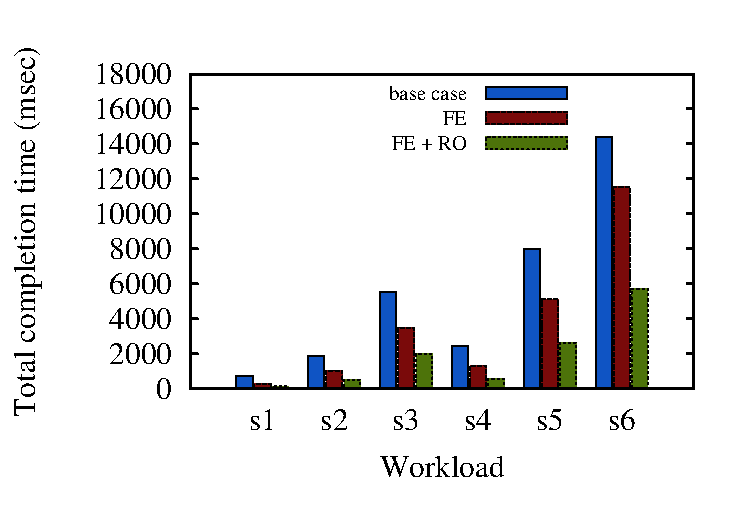
\includegraphics[width=0.55\textwidth]{figures/mazu/Failover-eps-converted-to.pdf}
\caption{Worst case flow setup time of affected flows in the failover
scenario with \BroadcomOne switches}\label{failoverResults}
\end{figure}

\begin{figure}
\centering
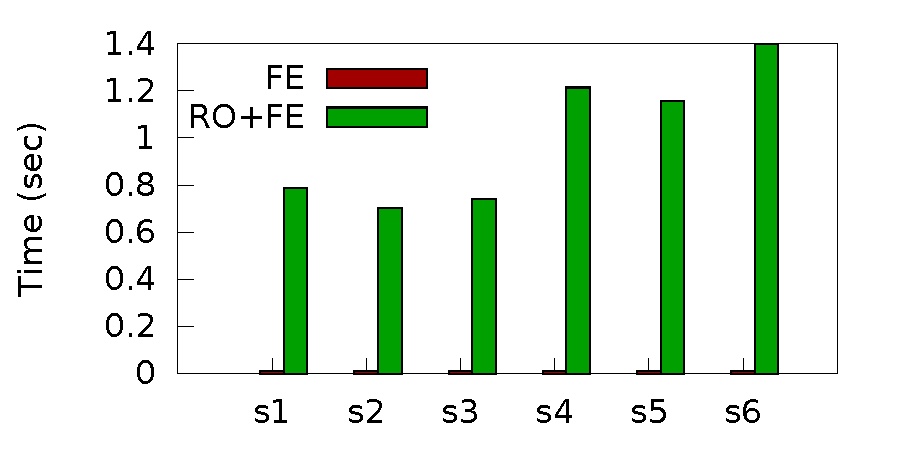
\includegraphics[width=0.55\textwidth]{figures/mazu/fe_ro_runtime.pdf}
\caption{Running time for FE and RO}
\label{runtime}
\end{figure}

\subsubsection{Two-level Responsive Traffic Engineering} 
Next, we evaluate the effectiveness of \FE and \RO in the
context of a control application that performs two-level responsive traffic
engineering. This application simultaneously routes two classes of
traffic---high and low priority---over the same network according to
different objectives. For low priority traffic, the objective is to minimize
the overall link utilization of the network due to this traffic; we install
coarse grained (wildcard) rules to route this traffic.  The objective for
high priority traffic is to minimize the overall link latency; we install
fine grained high priority rules to route this traffic. We first route the
low priority traffic, and then route the high priority traffic using the
remaining network capacity. We assume both categories of traffic can be
accommodated without causing any congestion. 

We use the same topology and workloads described in \secref{mazu:fe_eval}.
However, for high volume workloads (\sD-\sF) the volume of high priority and
low priority traffic between any two overlay nodes is about 17 and 200 flows,
respectively, and for low volume workloads (\sA-\sC) the volume is about 12
and 50 flows, respectively.

A network's ability to meet SLAs for each traffic class depends on how
quickly the network can establish routes when requests for both classes
arrive close in time.
\figsref{qos_Results}{qos_intelResults} show the total completion time using
\BroadcomOne and \Intel switches, respectively, with and without our
techniques. The base case has a significantly high flow set up time when the
number of low priority rules in the table are high: as high as 80s for
\BroadcomOne. This implies that ignoring flow setup latency can cost traffic
engineering dearly in terms of being responsive.  For low volume workloads
(\sA-\sC) the factor of improvement from just \FE is about 2.5X for
\BroadcomOne and 1.8X for \Intel, and with \FE+\RO it's about 5X for
\BroadcomOne and 4X for \Intel. We observe similar speedups for high volume
workloads (\sD-\sF). 

\begin{figure*}[!t]
\centering
        \begin{subfigure}[b]{0.40\textwidth}
                \centering
		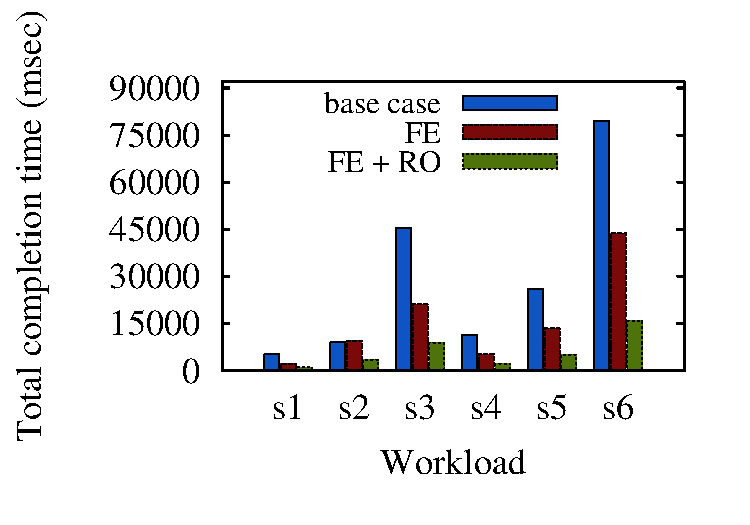
\includegraphics[width=\textwidth]{./figures/mazu/qos-eps-converted-to.pdf}
		\caption{Latency on \BroadcomOne switch}
		\label{qos_Results}
	\end{subfigure}
        \begin{subfigure}[b]{0.40\textwidth}
                \centering
		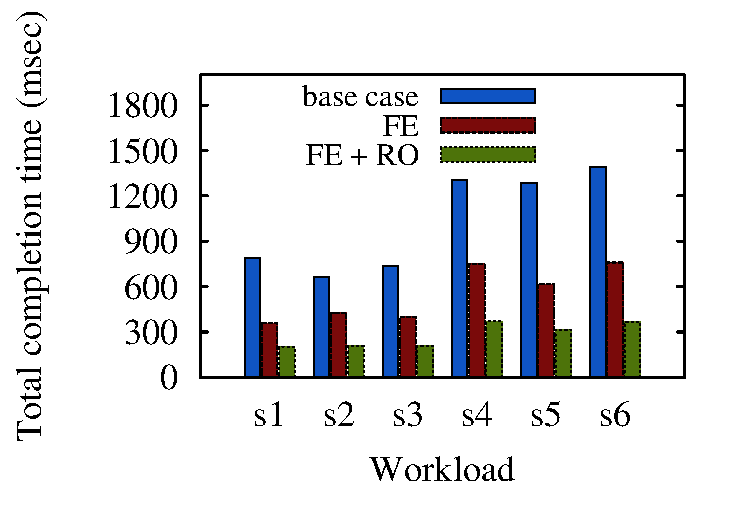
\includegraphics[width=\textwidth]{./figures/mazu/qos_intel-eps-converted-to.pdf}
		\caption{Latency on \Intel switch}
		\label{qos_intelResults}
	\end{subfigure}
	\caption{Worst case flow set up time in the two level traffic
    engineering scenario} 
	\label{qosResults}
\end{figure*}

\subsubsection{MicroTE}
MicroTE~\cite{benson2011microte} leverages the partial and short term
predictability of a data center traffic matrix to perform traffic engineering
at small time-scales. As noted in \secref{mazu-floweng}, \FE does not apply to
MicroTE since routes span a single tunnel and route changes all happen at a
single switch. Thus, MicroTE can only benefit from \RO, the extent of which we
now study.

We consider the following simple data center topology: we use a three-level FatTree topology~\cite{fattree} with degree 8, containing 128 servers connected by 32 edge, 32 aggregate, and 16 core switches.
We assume that the traffic rate between a pair of servers is derived from a
Zipfian distribution. \figref{microteResults} shows the rule installation
completion time. We see that \RO provides a 2X improvement (400ms to 200ms)
assuming the \BroadcomOne switch. Given the time-scales of predictability
considered, this can help MicroTE leverage traffic predictability longer,
thereby achieving more optimal routing. The improvement with \Intel is 1.6X
(80ms to 48ms).


\begin{figure}[!tb]
\centering
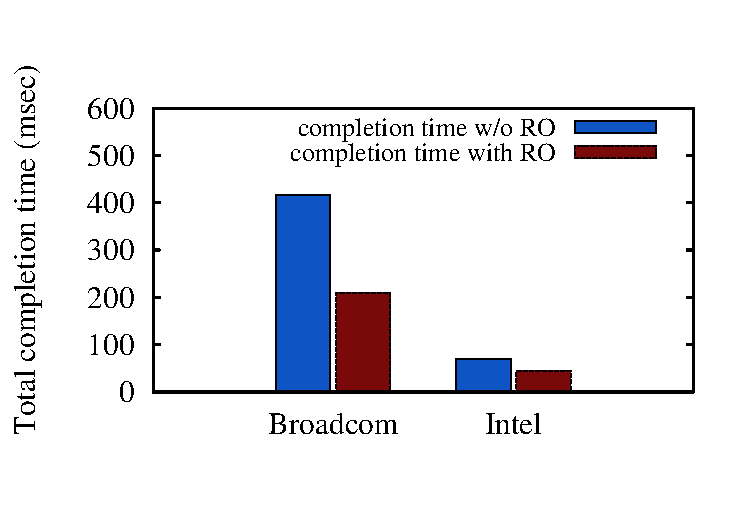
\includegraphics[width=0.55\textwidth]{./figures/mazu/MicroTE_Compl-eps-converted-to.pdf}
\caption{Flow setup time of MicroTE with and without \RO in a Fat Tree (k=8) topology}
\label{microteResults}
\end{figure}


%\subsection{Conclusion}
\label{mazu-conclusion}
Critical SDN applications such as fast failover and fine-grained traffic engineering demand
tight interaction between switch control and data planes. However, our
measurements across four OpenFlow-based switches show that the
latencies underlying the generation of control messages (\packetin's)
and execution of control operations (\flowmod's) can be quite high, and
variable. We find that the underlying causes are linked both to
software inefficiencies, as well as pathological interactions between
switch hardware properties (shared resources and how forwarding rules
are organized) and the control operation workload (the order of
operations issues, and concurrent switch activities). 
Our measurement study highlights the need of careful design of next generation switch silicon 
and software in order to fully utilize the power of SDN.
Finally, to mitigate the
challenges these latencies create for SDN in supporting critical
management applications, we present three measurement-driven techniques.
Our evaluation shows that these mechanisms can tame flow setup
latencies effectively, thereby enabling SDN-based control of critical
applications.



\section{Understanding Modern Web Service Deployment in EC2 and Azure}
\label{cloudmeasure}

\subsection{Introduction}
\label{cloudmeasure_intro}

An increasingly large fraction of Internet services are hosted
on a cloud computing system such as Amazon EC2 or Windows Azure.  But
to date, no in-depth studies about cloud usage by Internet services
has been performed. We provide a detailed
measurement study to shed light on how modern web service deployments use
the cloud and to identify ways in which cloud-using services might improve
these deployments. Our results show that:
4\% of the Alexa top million use EC2/Azure;
there exist several common deployment
patterns for cloud-using web service front ends;
and services can significantly
improve their wide-area performance and failure tolerance by
making better use of existing regional diversity in EC2.
Driving these analyses are several
new datasets, including one with over 34 million DNS records for
Alexa websites and a packet capture from a large university network.

\subsection{Measurement Scope \& Datasets}
\label{cloud-measure-background}


\begin{figure}[t]
\centering
\begin{subfigure}[b]{0.20\textwidth}
    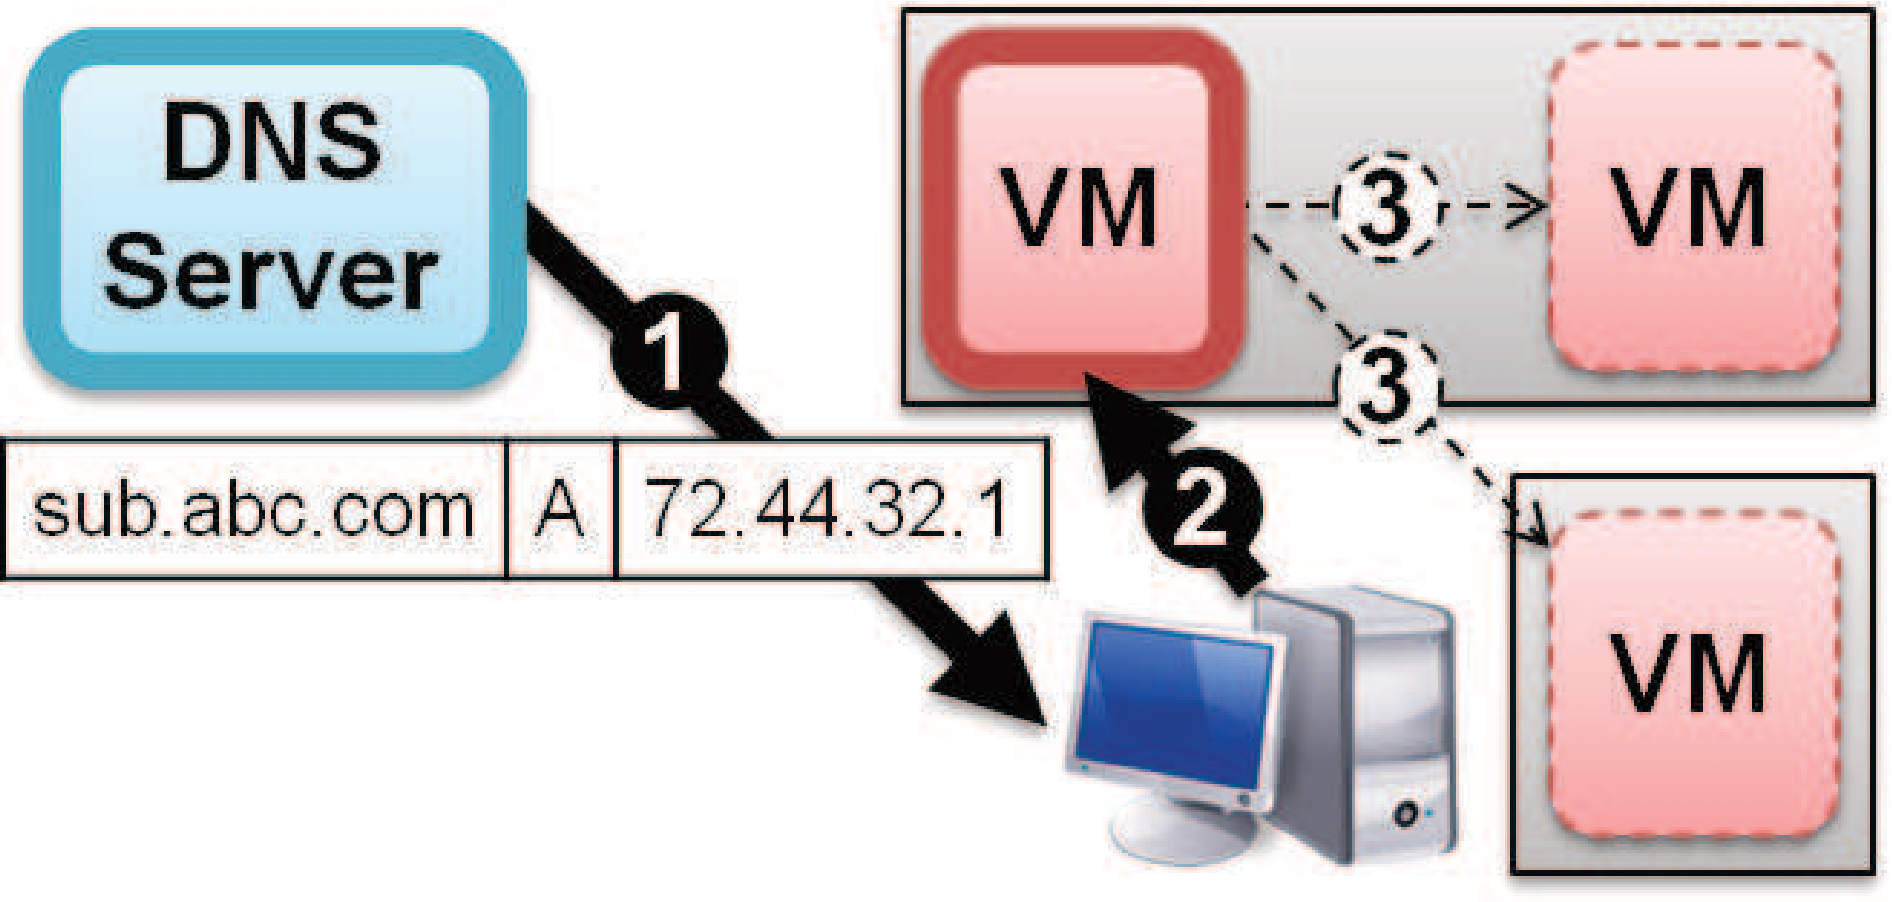
\includegraphics[width=\textwidth]{figures/cloudmeasure/imag_sec2/ec2_vm.pdf}
    \caption{P1: VM front end}
    \label{fig:ec2_vm}
\end{subfigure}
\hspace{0.03\columnwidth}
\begin{subfigure}[b]{0.3\textwidth}
    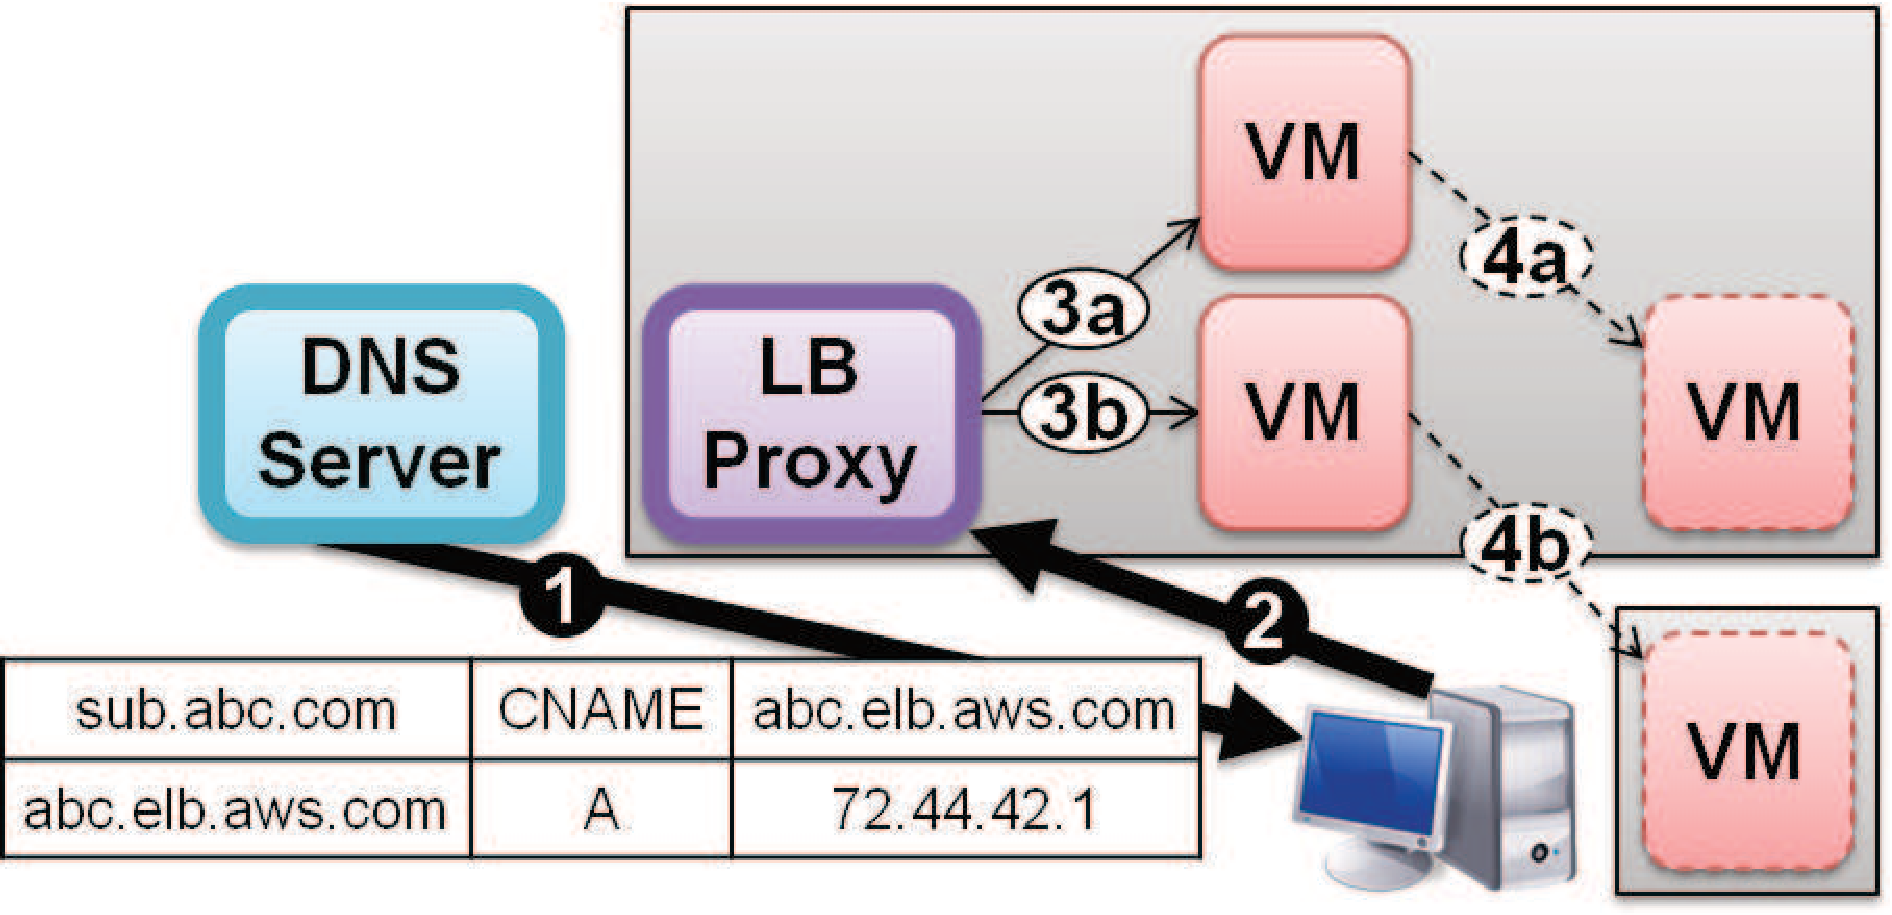
\includegraphics[width=\textwidth]{figures/cloudmeasure/imag_sec2/ec2_elb.pdf}
    \caption{P2: Load balancer front end}
    \label{fig:ec2_elb}
\end{subfigure}

\begin{subfigure}[b]{0.20\textwidth}
    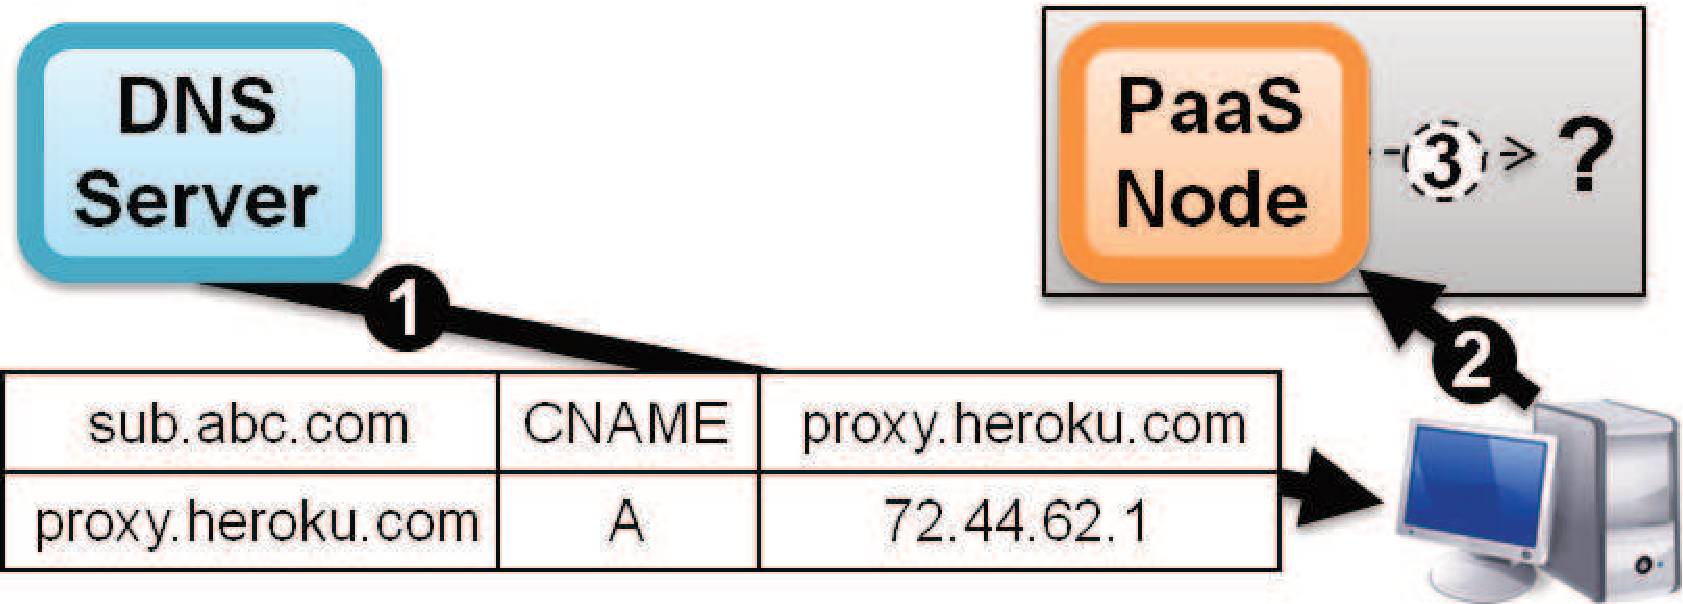
\includegraphics[width=\textwidth]{figures/cloudmeasure/imag_sec2/ec2_heroku.pdf}
    \caption{P3: PaaS front end}
    \label{fig:ec2_paas}
\end{subfigure}
\hspace{0.03\columnwidth}
\begin{subfigure}[b]{0.30\textwidth}
    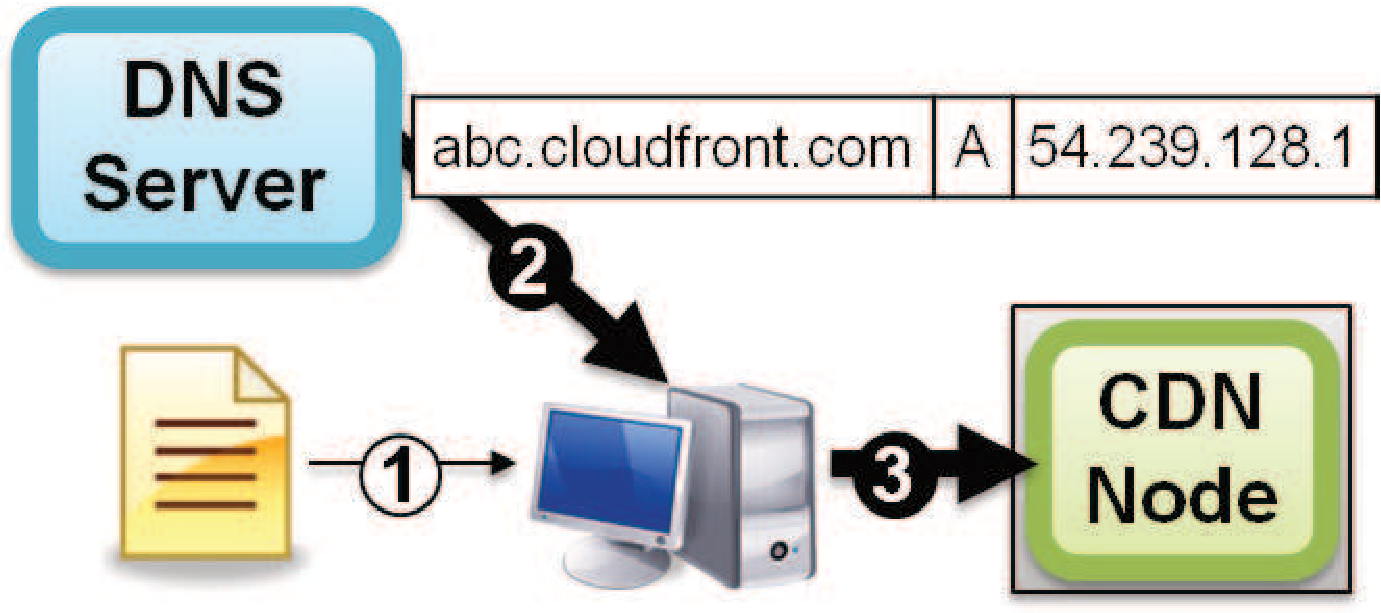
\includegraphics[width=\textwidth]{figures/cloudmeasure/imag_sec2/ec2_cdn.pdf}
    \caption{P4: Leverage CDN}
    \label{fig:ec2_cdn}
\end{subfigure}

\caption{Deployment patterns for web services.}
\label{fig:ec2_models}

\end{figure}


Public IaaS clouds, such as Amazon EC2, Windows Azure, and Rackspace,
allow tenants to dynamically rent virtual machine (VM) instances with
varying CPU, network, and storage capacity. Cloud tenants have the
option of renting VMs in one or more geographically distinct
data centers, or {\em regions}. Some clouds, such as EC2,
further divide these regions into multiple distinct availability {\em
  zones}. Each zone has separate compute and power
infrastructure to make certain failure modes zone-specific and to
allow cloud tenants to replicate their deployments across
multiple zones for smooth fail-over.

Beyond simple VMs, IaaS providers, as well as third parties, offer a
wide-range of value-added features: load balancers (e.g., Amazon
Elastic Load Balancer and Azure Traffic Manager),
plat\-form-as-a-service environments (e.g., Amazon Elastic
Beanstalk, Heroku, and Azure Cloud Services), content-distribution networks
(e.g., Amazon CloudFront and Azure Media Services), DNS hosting (e.g.,
Amazon route53), etc. The result is a complex ecosystem of
interdependent systems operating at multiple layers of abstraction,
and, in turn, a large variety of possible deployment patterns for
cloud tenants. In this paper, we study four popular deployment patterns. We
describe these using a series of examples.

In \figref{fig:ec2_models}, we show the steps involved in a client
accessing an EC2-hosted web service that is using one or more of the
aforementioned features. When a client wants to access a web service,
it first performs a DNS lookup of the service's domain name.  The
response may contain an IP address associated with a VM (deployment
pattern {\em P1}), a load balancer ({\em P2}), or a
platform-as-a-service (PaaS) node ({\em P3}).
With {\em P2}, the client request is subsequently directed to a
VM\footnote{Or PaaS
  nodes, as is done by Amazon Elastic Beanstalk and Azure Traffic
  Manager.}. Tenants using {\em P1}--{\em P3} may also rely on
additional VMs or systems (dashed lines) to handle a
client's request; these additional components may or may not be in the
same region or availability zone (indicated by the gray boxes). An
object returned to a client (e.g., a web page) may sometimes require
the client to obtain additional objects (e.g., a video) from a
content-distribution network ({\em P4}).

We focus on studying the front end portions of web
service deployments within the above four deployment patterns (indicated by 
the thicker lines in \figref{fig:ec2_models}). These
portions are encountered within the initial few steps of a client
making a request. We leave an exploration of deployment/usage patterns
covering the later steps (e.g. back-end processing) for future work.


\subsubsection{Datasets}
\label{cloud-measure-datasets}

We use two primary datasets: ({\em i}) a list of cloud-using
subdomains derived from Alexa's list of the top 1 million websites,
and ({\em ii}) packet traces captured at the border of the
UW-Madison campus network. Both datasets leverage the fact that EC2~\cite{ec2iprange}
and Azure~\cite{azureiprange} publish a list of the public IPv4
address ranges associated with their IaaS cloud offerings. Below, we
provide details on our \alexadata and \capturedata datasets. We
augment these data sets with additional traces and active measurements
to aid specific analyses; we describe these at the appropriate places
in subsequent sections.


\tightparagraph{Top Cloud-Using Subdomains Dataset}
Our first dataset is a list of subdomains which use EC2 or Azure and are 
associated with domains on Alexa's list of the top 1 million
websites~\cite{alex_topdomains}. We consider a subdomain to use EC2 or Azure if a
DNS record for that subdomain contains an IP address that falls within EC2 or
Azure's public IP address ranges. 

To construct this dataset, we first identified the subdomains associated with
each domain on Alexa's list of the top 1 million websites.  We started
with Alexa's top 1 million list from Feburary 6, 2013 and attempted to issue
a DNS zone transfer (i.e., a DNS query of type AXFR) for each domain on the
list.  The query was successful for only about 80K of the domains.  For the
remaining domains, we used dnsmap~\cite{dnsmap} to identify subdomains by
brute-force. Dnsmap uses a pre-defined word list, which we augmented with the
word list from knock~\cite{knock}, to construct potential subdomain names.
Dnsmap then runs DNS queries to check if the potential subdomains actually 
exist. This brute-force approach misses some subdomains,
but it allows us to provide a lower bound on the number of subdomains which 
use public IaaS clouds and explore the deployment patterns of these known 
cloud-using subdomains.
We distributed this task to 150 globally-distributed PlanetLab
nodes, producing a list of 34 million valid subdomains.

To limit the list of subdomains to cloud-using subdomains, we performed a series of
DNS lookups using the UNIX dig utility. We first performed a single
DNS lookup from one PlanetLab node (chosen from our set of 150 nodes)
for each subdomain. If the DNS record contained an IP address within
EC2 or Azure's public IP ranges\footnote{We assume the IP address ranges 
published by EC2 and Azure are relatively complete.}, we included it on our 
list of the top
cloud-using subdomains. This resulted in a list of 713K cloud-using
subdomains. We then performed a DNS lookup for each of the cloud-using
subdomains on every node in a set of 200 globally-distributed
PlanetLab nodes. \figref{fig:nodes_deploy} shows the geographic location of 
these PlanetLab nodes, which are spread across North America, South America,
Europe, Asia, and Australia.
The queries were performed March 27-29,
2013. These distributed DNS queries help ensure that we gather a
comprehensive set of DNS records for each cloud-using subdomain and
capture any geo-location-specific cloud usage.

We refer to the list of cloud-using subdomains, and their associated
DNS records, as the \alexadata dataset. 


 \begin{figure}[tb]
 \centering
 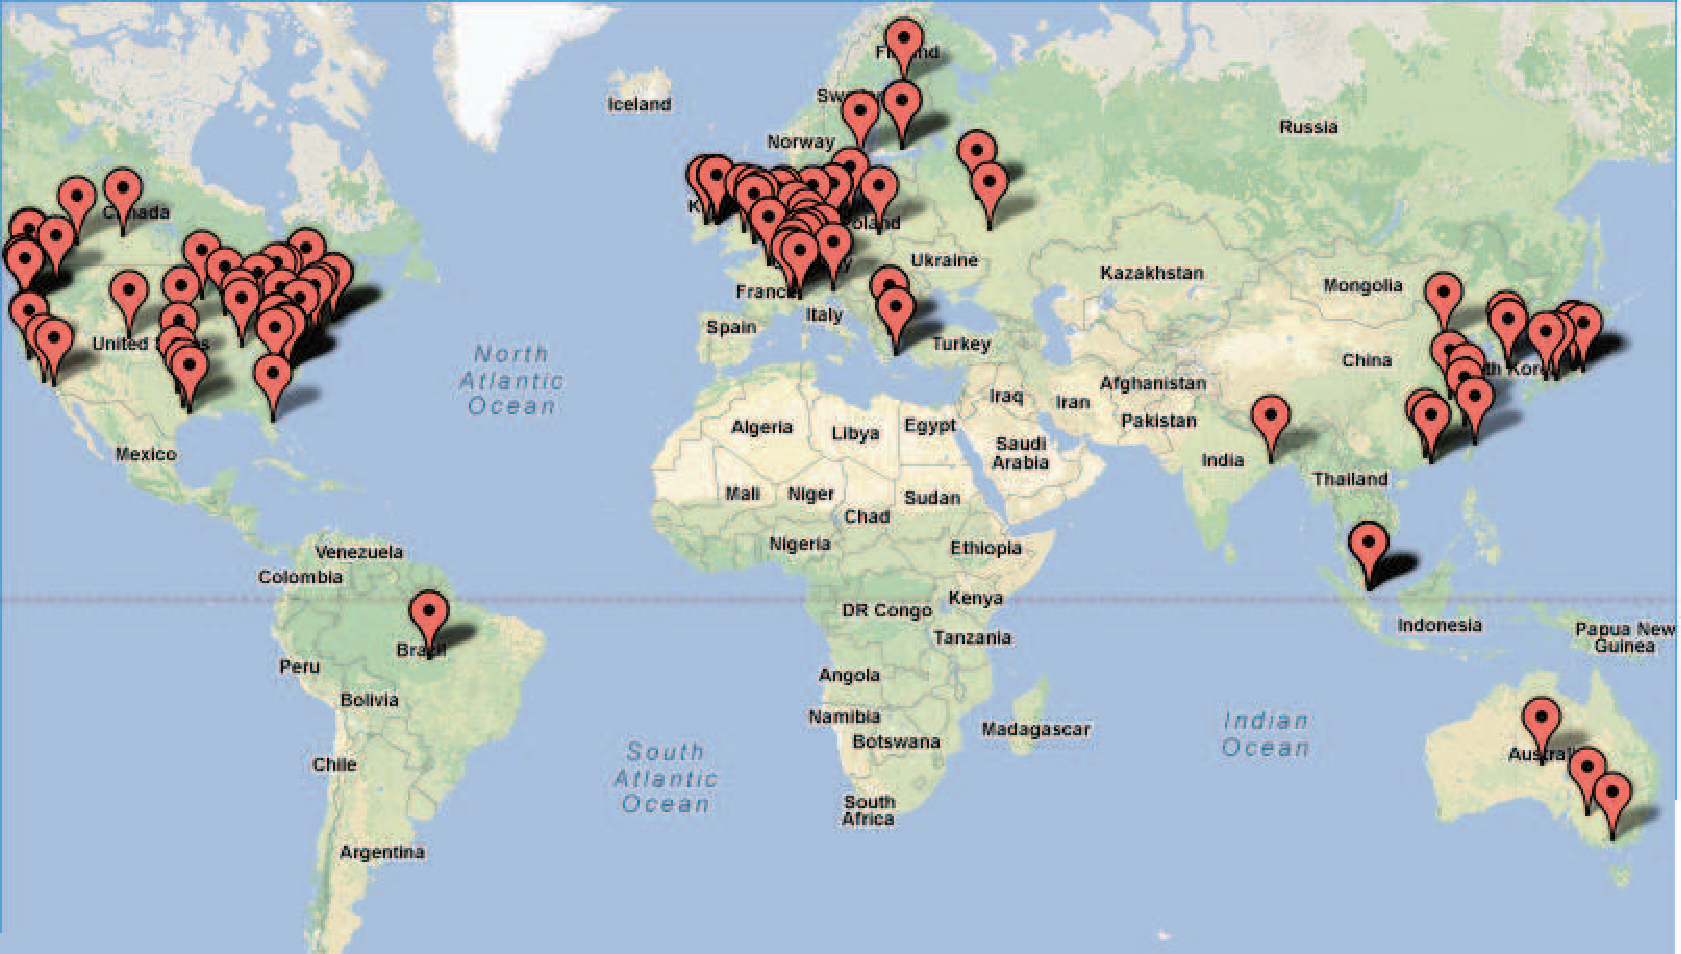
\includegraphics[width=0.55\columnwidth]{figures/cloudmeasure/imag_sec2/nodes_deploy.pdf}
 \caption{PlanetLab nodes used for DNS lookups\label{fig:nodes_deploy}}
 \end{figure}

%%%%%%%%%%%%%%%%%%%%%%%%%%%%%%%%%%%%%%%%%%%%%%%%%%%%%%%%%%%%%%%%%%%%%%%%%%%%%

\tightparagraph{Packet Capture Dataset} Our second primary dataset is a
series of packet traces captured at the border of the University of
Wisconsin-Madison campus network\footnote{The university has seven /24 IP blocks and one /16
IP block}. We captured full IP packets whose source or destination IP
address fell within the public address ranges published by EC2 and
Azure. The capture was performed from Tuesday, June 26 to Monday, July
2, 2012 giving us a full week of traffic and a total of 1.4TB of data.
The total Internet traffic averaged approximately 7Gbps during the capture,
with about 1\% of the traffic going to/coming from EC2 or Azure. Due to the
relatively low rate of traffic being captured, no loss occurred during the
capture process (according to tcpdump and counters reported by the border
router). 
To protect user privacy, we anonymized the IP addresses of clients
within the university network, and we only report aggregate
statistics.

Since our traces contain full packets, we were able to perform an
in-depth analysis of network and transport layer information (e.g., IP
addresses, protocols, ports), application layer information (e.g.,
HTTP hostnames, HTTP content-type, HTTPS certificates), and packet
payloads. We extracted relevant information from the traces using
Bro~\cite{paxson1998bro}, a network monitoring and traffic analysis
tool. We refer to these traces as the
\captureonedata dataset.



%%%%%%%%%%%%%%%%%%%%%%%%%%%%%%%%%%%%%%%%%%%%%%%%%%%%%%%%%%%%%%%%%%%%%%%%%%%%%



\subsection{Web-Facing Cloud Tenants}
\label{cloud-measure-who}

In this section, we explore what 
applications are being hosted on public IaaS clouds.
We start by analyzing the packet capture to identify the types of applications
being hosted. This analysis suggests (unsurprisingly) that web applications 
represent a large, important set of cloud tenants.
We then turn to examining which of the most popular websites 
are using clouds. We view popularity both globally, via
the Alexa top website  rankings, and locally, via 
the volume of traffic associated with each domain in the packet capture. 

%%%%%%%%%%%%%%%%%%%%%%%%%%%%%%%%%%%%%%%%%%%%%%%%%%%%%%%%%%%%%%%%%%%%%%%%%%%%%%%%
\subsubsection{Protocols and Services}
\label{sec:protocols}

\begin{table}[!t]\small
\centering
\input{cloudmeasure_tables/tab_capture_cloudsplit}
\caption{Percent of traffic volume and percent of flows associated with
    each cloud in the packet capture.}
\label{tab:cloudsplit}
\end{table}

\begin{table}[!t]\small
\centering
\input{cloudmeasure_tables/tab_capture_protocols}
\caption{Percent of traffic volume and percent of flows associated with each  
    protocol in the packet capture.}
\label{tab:proserv}
\end{table}

We first examine the fraction of bytes and flows in the \capturedata that are
associated with each cloud (\tabref{tab:cloudsplit}). We only consider flows
that were initiated within the university and destined for EC2 or Azure.
We observe that the majority of cloud traffic, both as measured by volume and
number of flows, is EC2-related: 81.73\% of bytes (80.70\% of flows)
are associated with EC2, while Azure accounts for 18.27\% of bytes
(19.30\% of flows).

Next, we use the \capturedata to study the application-layer protocols used by cloud tenants.
\tabref{tab:proserv} shows the
percentage of bytes (and flows) using a specific protocol relative to the
total number of bytes (and flows) for EC2, Azure, and the capture as a whole.

We observe that more than $99\%$ of bytes in the \captureonedata 
are sent and received using TCP, with less than $1\%$ of bytes
associated with UDP or ICMP.  The vast majority of this TCP traffic is
HTTP and HTTPS. The proportion of HTTPS traffic is far higher than
that seen for general web services in the past (roughly
6\%~\cite{agarwal2010endre}); as we will show later, HTTPS traffic is dominated
by cloud storage services. Interestingly, the majority of Azure's TCP traffic
is HTTP (59.97\%) while the majority of EC2's TCP traffic is HTTPS (80.90\%)  

The breakdown by flow count is less skewed
towards TCP, with UDP flows accounting for 14\% of flows in the
\captureonedata. This is largely due to DNS queries, which account for
11\% of flows but carry few bytes.

As one would expect, public IaaS clouds are also used for non-web-based
services.  In the \captureonedata, we find a small fraction of non-HTTP(S)
TCP traffic and non-DNS UDP traffic going to both EC2 and Azure. 
This traffic includes SMTP, FTP, IPv6-in-IPv4, SSH, IRC, and other traffic that Bro
could not classify.


\tightparagraph{Summary and implications} While we analyze a single
vantage point, our measurements suggest that web
services using HTTP(S) represent an important set of WAN-intensive
cloud tenants. The extent to which compute-intensive workloads (that
may not result in a large impact on network traffic) are prevalent as
cloud tenants remains an interesting open question.  In the following
sections we dig into what tenants are hosting web services on public
clouds as well as diving deeper into their traffic patterns.



\subsubsection{Popular Cloud-Using (Sub)Domains} 
\label{cloud-measure-global}

\tightparagraph{Cloud-using Alexa domains} We now consider what subset of the 
Alexa top 1 million websites use the cloud to (partly) host their services. 
Recall that Alexa provides an estimate of the most
popular domains worldwide. Their ranking is based on the number of unique
visitors and the number of page views over the last 3 months, aggregated at the
domain level\footnote{Except for domains hosting personal sites, e.g.,
\myurl{wordpress.com}, where subdomains are ranked
individually.}~\cite{alex_topdomains}.  
Using our \alexadata dataset, we can determine which Alexa sites are hosted in
EC2/Azure.
%Determining the reliance on EC2/Azure
%of  such popular sites  allows us to assess the extent
%this macroscopic perspective on website popularity 
%to begin to quantify what web domains use public IaaS clouds.

We find that 40,333 ($\mathord{>}4\%$) of the domains on Alexa's top 1 million
list have a subdomain that uses EC2 and/or Azure.
Under these domains, there are a
total of 713,910 cloud-using subdomains. 
Note that these are lower bounds on cloud use, since our
analysis approach (see \S\ref{cloud-measure-datasets}) means we do not flag as
cloud-using any domains that use a layer of indirection (e.g., via services
like CloudFlare~\cite{cloudflare}) before requests are sent to EC2 or Azure. 

\tabref{tab:hybrid_cloud} provides a breakdown of the domains and
subdomains in terms of whether they use EC2, Azure, or other hosting
services (the last indicating
IP addresses not associated with EC2 or Azure).  Note that ``other''
could in fact be public clouds besides EC2 and Azure. 
A subdomain is marked as {\em EC2 only} if it always resolves only to IP 
addresses within EC2; similarly for Azure. We mark a subdomain as {\em
EC2+Azure}, {\em EC2+Other}, or {\em Azure+Other} if it resolves to IP 
addresses associated with the appropriate subset of EC2, Azure, and other.
Domains are counted as {\em EC2 only}
if all of their subdomains only use EC2; similarly for Azure. Domains are 
marked as {\em EC2+Azure}, {\em EC2+Other}, or {\em Azure+Other} if they have 
subdomains associated with
the indicated subset of EC2, Azure, and other. 

\begin{table}[!t]
\centering
\small
\input{cloudmeasure_tables/tab_cloud-using_alexa}
\caption{Breakdown of domains and subdomains based on their use of EC2, 
    Azure, and/or other hosting services.}
\label{tab:hybrid_cloud}
\end{table}





The vast majority of cloud-using domains (94.9\%) use EC2, and the majority of
these domains use other hosting for some of their subdomains (i.e., EC2 + Other).  
{Only 5.8\% of domains use Azure.  Additionally, a small
fraction (0.7\%) of cloud-using domains use both EC2 and Azure; hence
the {\em EC2 total} and {\em Azure total} rows in \tabref{tab:hybrid_cloud}
sum to more than 100\%.
A list of the top 10 (by Alexa rank) EC2-using domains 
appears in \tabref{tab:top-15}. This list will be used in several later 
sections with results specific  to EC2, which is why we excluded the four 
top Azure domains 
that would otherwise have been in the top~10: \myurl{live.com}, \myurl{msn.com}, \myurl{bing.com}, and \myurl{microsoft.com}.

The distribution of Alexa ranks for cloud-using domains 
is skewed: higher ranked domains are more likely 
to be cloud-using than lower ranked domains. 
%a larger fraction of higher-ranked domains use EC2 and/or Azure
%compared to lower-ranked domains 
%Figure~\ref{fig:cdf-alexa} shows a CDF of the percentage of cloud-using 
%domains with rank less than or equal to the indicated x-axis values. 
Notably, 42.3\% of cloud-using domains have ranks in 
the first 250,000 sites versus only 16.2\% of the bottom 250K domains. 
%In Figure~\ref{fig:top-15} we list the top 15 EC2-using 
%Alexa domains, and the number of subdomains they use both 
%in and out of the cloud. 

The most frequent prefix used by cloud-using subdomains in our Alexa 
subdomains dataset is \myurl{www} (3.3\% of all cloud-using subdomains). The other top 10 prefixes
(each $\mathord{<}1\%$) are, in order:
\myurl{m}, \myurl{ftp}, \myurl{cdn}, \myurl{mail},
\myurl{staging}, \myurl{blog}, \myurl{support}, \myurl{test}, and \myurl{dev}.
%A small handful of domains use both EC2 and Azure. 
The majority of subdomains are hosted either only in
the cloud or only elsewhere, although a small fraction (3\%) appear to be
hosted both on EC2 and other providers,
what we might call a hybrid-cloud deployment.







\begin{table}[!t]
\center
\small
\input{cloudmeasure_tables/tab_top15_subdomains}
\caption{Top 10 (by Alexa rank) EC2-using domains, their total number of subdomains, and the
number of EC2-using subdomains.} 
\label{tab:top-15}
\end{table}

\begin{table*}[!t]
\centering
\small
\input{cloudmeasure_tables/tab_capture_top_combined}
\caption{Domains with highest HTTP(S) traffic volumes (in GB) in the \captureonedata.
Percentages are relative to the total HTTP(S) traffic across both clouds in the capture. Domains marked with 
($\deepfield$) appeared on DeepField's Top 15~\cite{deepfield}.}
\label{tab:topdomains}
\end{table*}

\tightparagraph{High traffic volume domains}
We complement the above with an analysis of the top domains seen in 
the \captureonedata, as measured by traffic volume.  
We use Bro to extract 
hostnames within HTTP requests and common names within the server
certificates embedded in HTTPS flows\footnote{TLS
encryption hides the hostname associated with the underlying HTTP
requests, so we use the common names found in TLS server
certificates as a proxy.}. Aggregating the hostnames and common
names by domain, we find 13,604 unique cloud-using domains:
12,720 use EC2 and 885 use Azure.  Of these 13,604 domains, 6902 were also
identified as cloud-using via the Alexa dataset; the remainder were not in
the Alexa top 1 million.
\tabref{tab:topdomains} lists the highest 15 such 
domains in terms of traffic volume. A few tenants 
are responsible for a large fraction of the traffic. Most notably, 
\myurl{dropbox.com} accounts for almost 70\% of the combined HTTP(S) traffic volume. 
This also explains why HTTPS (used by \myurl{dropbox.com}) dominates HTTP 
in terms of volume (though not number of flows, refer to
        \tabref{tab:proserv}). 


It is informative to compare our analysis of top EC2-using domains by traffic
volume to the analysis by DeepField networks~\cite{deepfield}, 
which was conducted three months
before we collected the \captureonedata. They used data from
customers of their network analysis products. Seven of the domains on our top
15 list also appear within the top 15 on DeepField's list (indicated with a
        ($\deepfield$) in \tabref{tab:topdomains}).

\tightparagraph{Summary and implications} A substantial fraction of the
world's most popular websites rely in whole or in part on public IaaS
clouds, especially EC2.  Most cloud-using domains have some subdomains
hosted on a cloud service while other subdomains are hosted elsewhere.
Perhaps surprisingly a small, but noticeable fraction of subdomains
use both a cloud and other hosting solutions. Finally, traffic volume
appears to be dominated by a few cloud tenants (we discuss traffic
patterns more next). Depending on how tenants' deploy their services
(e.g., how many and which regions they use), these observations have
implications for availability of web-based cloud-resident services. We
explore the underlying deployments in more detail in \secref{cloud-measure-how}.


%%%%%%%%%%%%%%%%%%%%%%%%%%%%%%%%%%%%%%%%%%%%%%%%%%%%%%%%%%%%%%%%%%%%%%%%%%%%%

%\subsection{Traffic Patterns}
\label{cloud-measure-local}

\begin{figure}[!t]
\centering

%\minipage{0.31\textwidth}
\begin{subfigure}[b]{0.23\textwidth}
	\caption{HTTP flow count}
    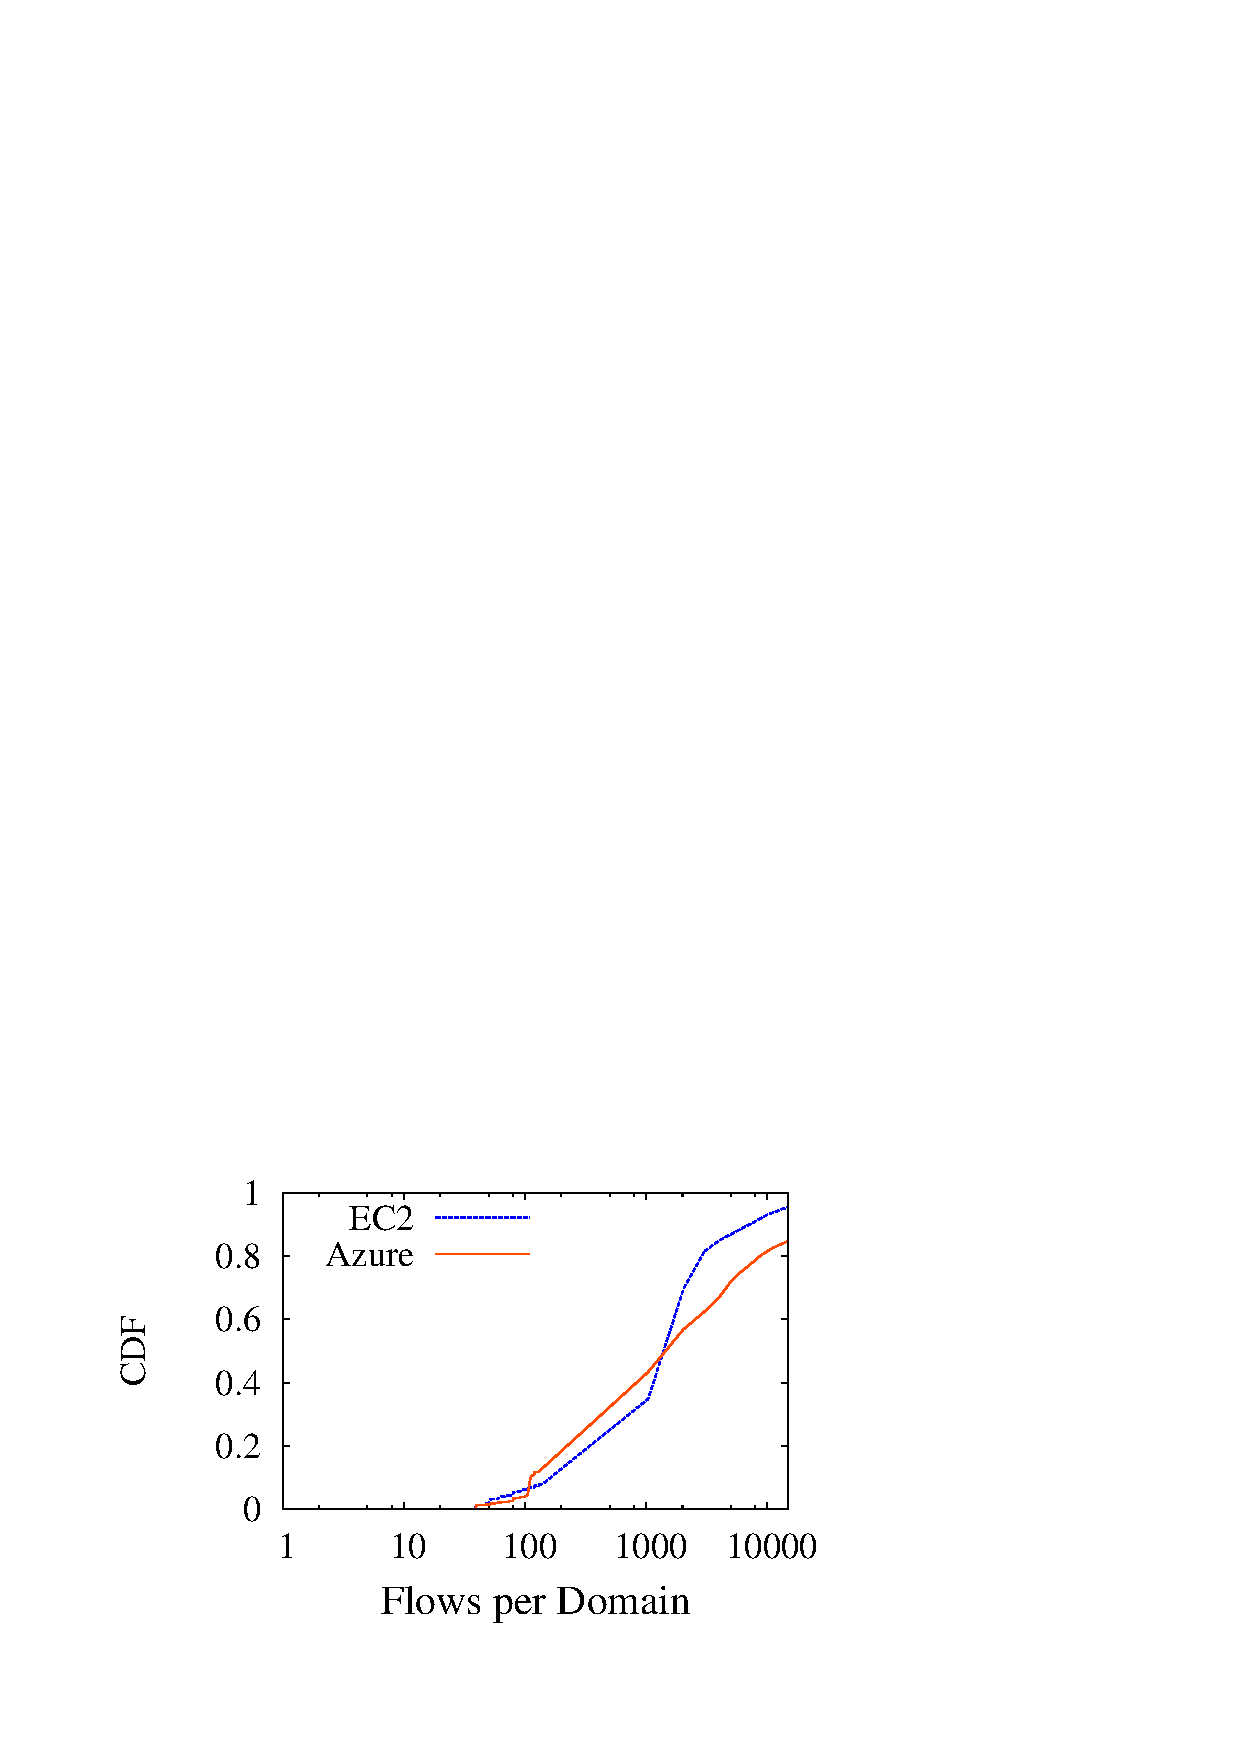
\includegraphics[width=\linewidth]{figures/cloudmeasure/imag_sec2/http_flow_cdf.pdf}
    \label{fig:httpflow-cdf}
\end{subfigure}
\begin{subfigure}[b]{0.23\textwidth}
    \caption{HTTPS flow count}
	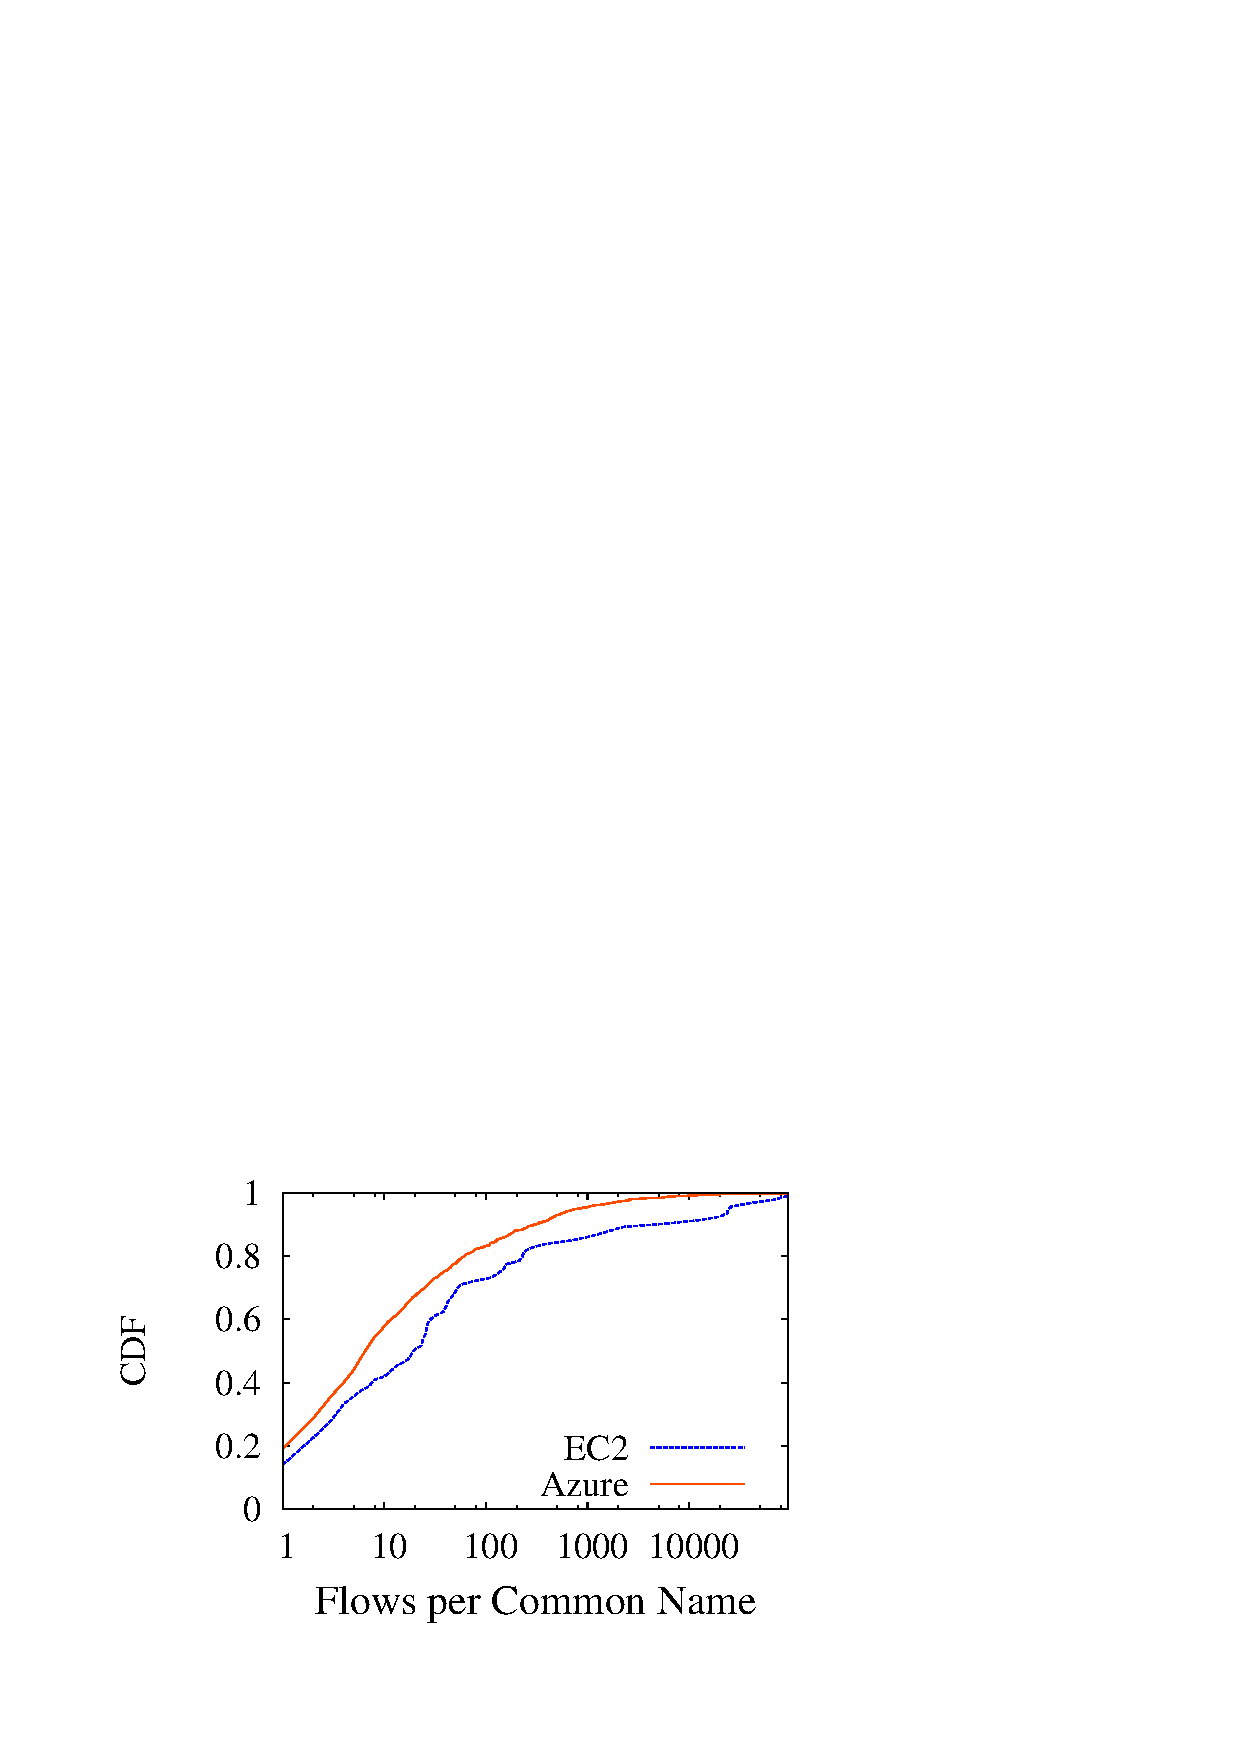
\includegraphics[width=\linewidth]{figures/cloudmeasure/imag_sec2/https_flow_cdf.pdf}
    \label{fig:httpsflow-cdf}
\end{subfigure}
\begin{subfigure}[b]{0.23\textwidth}
    \caption{HTTP flow size}
    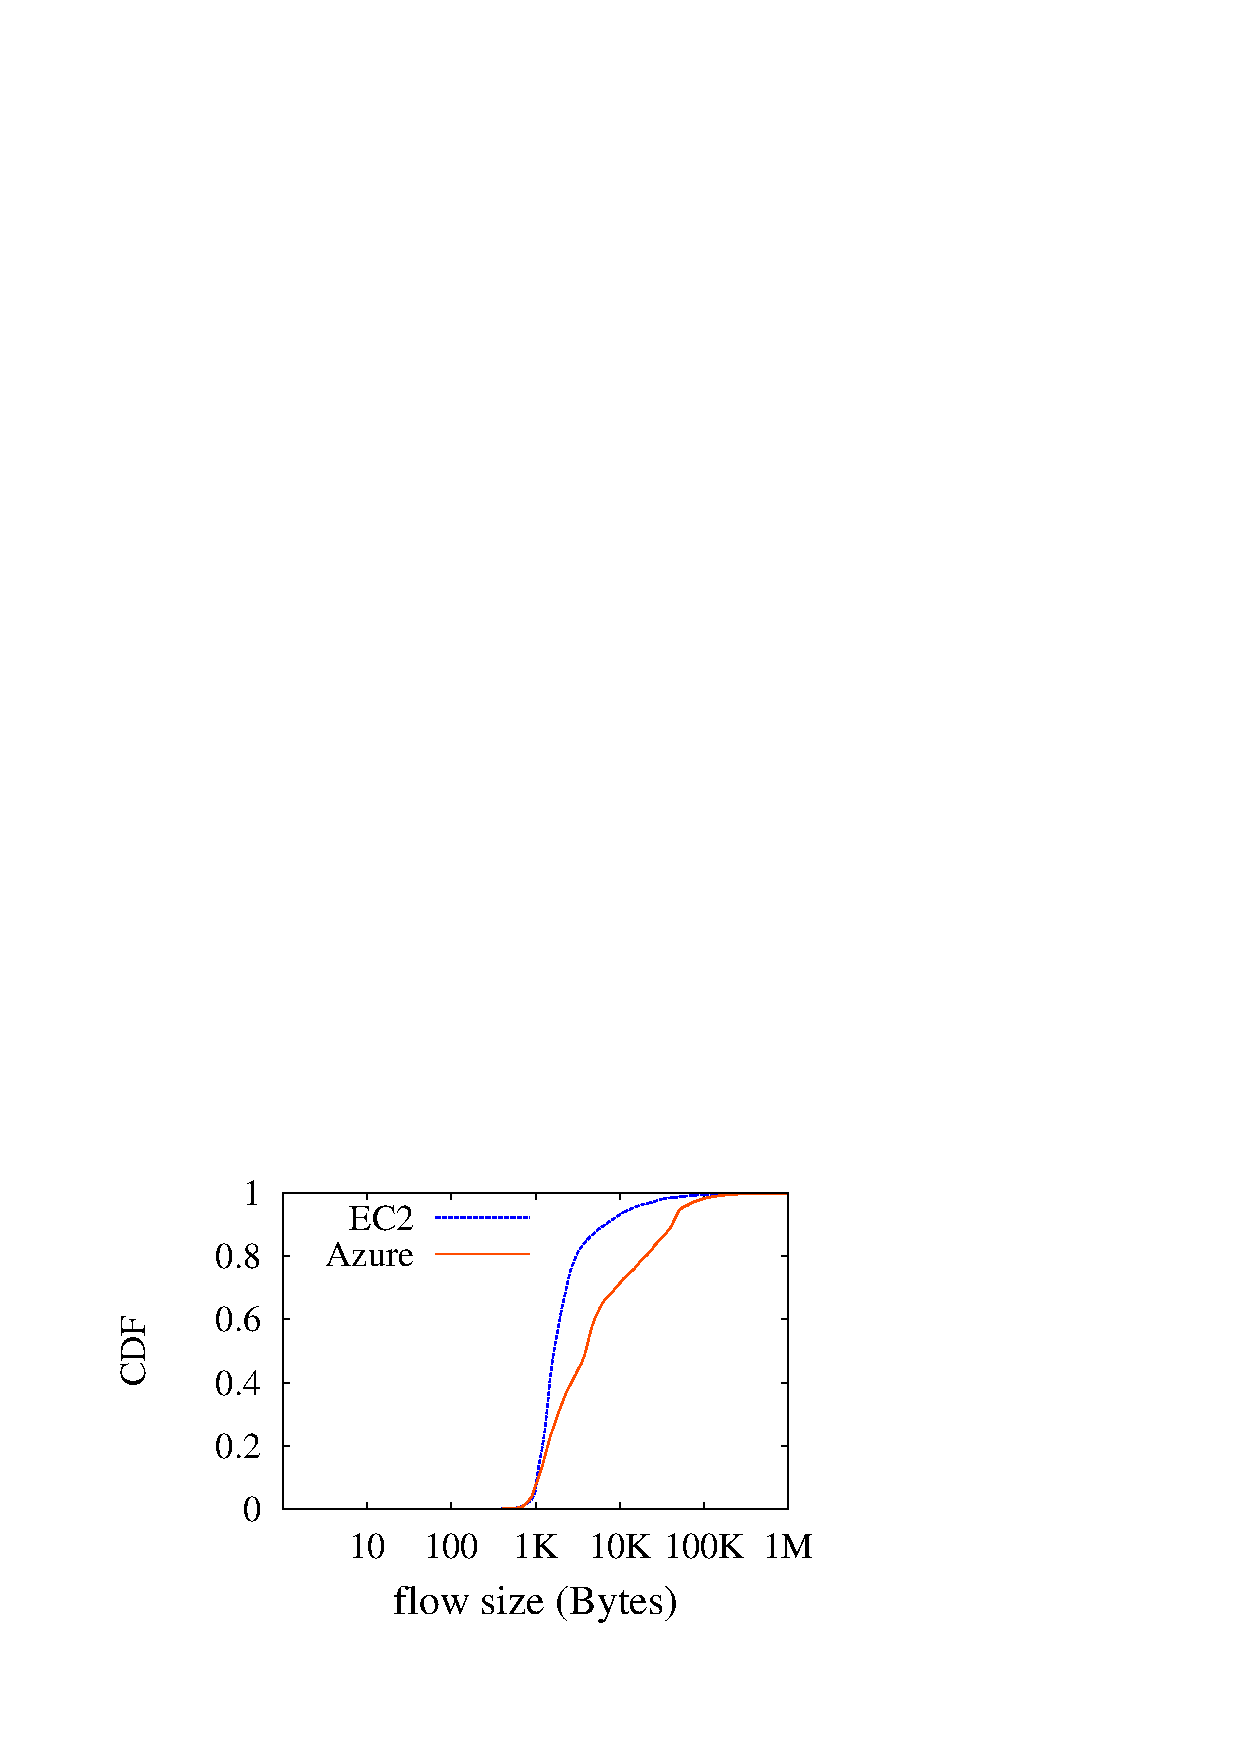
\includegraphics[width=\linewidth]{figures/cloudmeasure/imag_sec2/http_flow_size_cdf.pdf}
    \label{fig:http-flow-size-cdf}
\end{subfigure}
\begin{subfigure}[b]{0.23\textwidth}
    \caption{HTTPS flow size}    	
	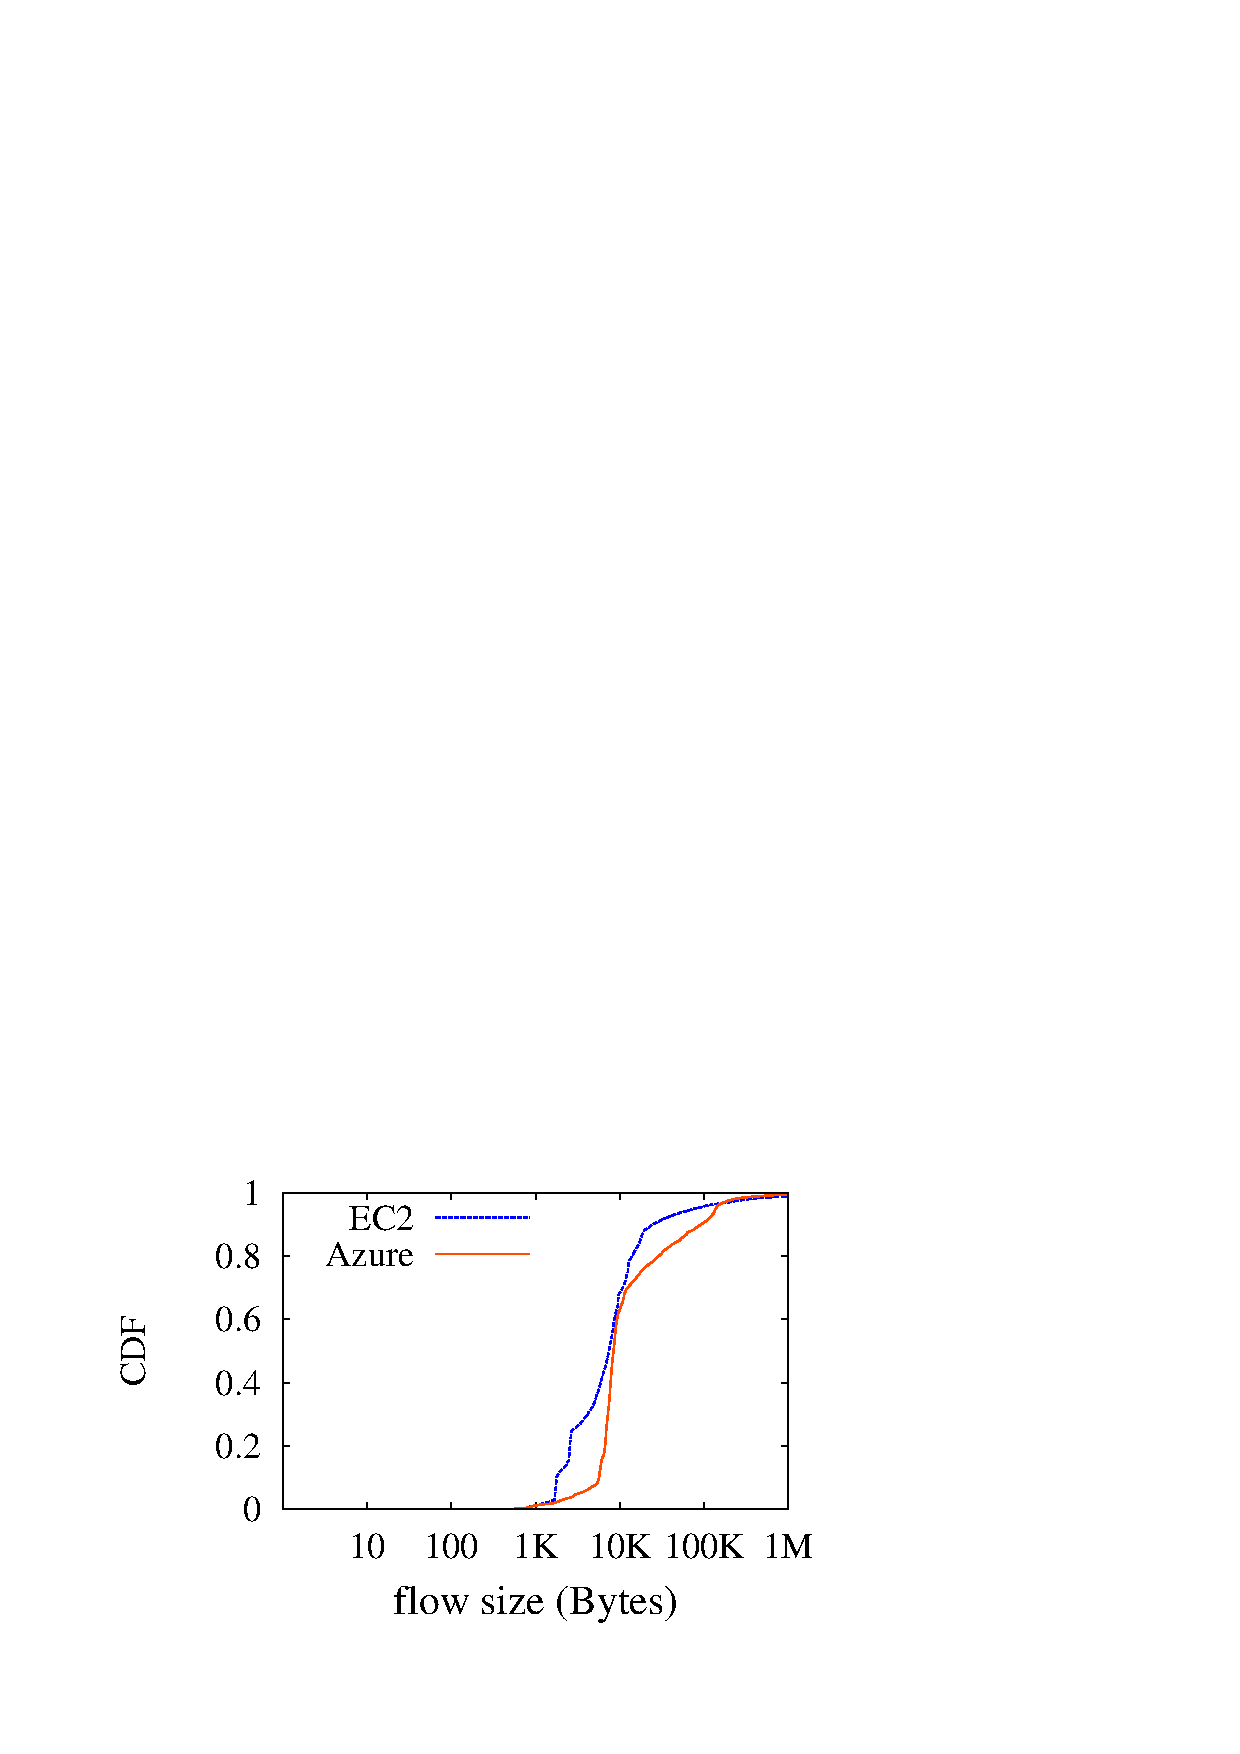
\includegraphics[width=\linewidth]{figures/cloudmeasure/imag_sec2/https_flow_size_cdf.pdf}
    \label{fig:https-flow-size-cdf}
\end{subfigure}

\caption{CDFs for HTTP/HTTPS flow counts and sizes.}
\label{fig:traffic-pattern}
\end{figure}


Our \captureonedata enables us to analyze not only who is running on the
cloud, but also the traffic patterns between clients in our university and 
cloud-resident web services.


\minisection{Flow-level properties} 
We first study the number of flows observed for various cloud-using domains 
in the \captureonedata. Figures~\ref{fig:httpflow-cdf} and
\ref{fig:httpsflow-cdf} show CDFs of the number of HTTP and HTTPS flows,
respectively, per-domain across our entire \captureonedata.  We observe that
$\approx$50\% of domains have fewer than 1,000 HTTP flows, and more than 80\%
of domains have fewer than 1,000 HTTPS flows.  Upon further analysis, we
found that the top 100 cloud-using domains are responsible for about 80\% of
the HTTP flows in EC2, and nearly 100\% of the HTTP flows in Azure; a long
tail follows for both clouds (CDF excluded for brevity). 

Flow sizes and durations generally appear to fit heavy-tailed
distributions (we omit durations in \figref{fig:traffic-pattern} for
brevity); similar properties have been observed for flows in other
networking contexts (e.g., in data
centers~\cite{benson2010network}). We note interesting differences
between HTTP and HTTPS: in particular, HTTPS flows are larger and last
longer than HTTP flows across both EC2 and Azure (e.g., median sizes
for EC2 are 10K and 2K, respectively).  This is expected given our
observation that a large percentage of HTTPS traffic is from file
storage services. In both cases, we see large flows that are more than a
few MB in size and long flows that last for a few hours.










\subsection{Tenants' Deployment Posture}
\label{cloud-measure-how}

In this section, we attempt to understand {\em how} tenants use
the cloud for deploying their front ends. We start by analyzing the deployment patterns employed by
cloud-using (sub)domains.  We first focus on the four 
patterns identified in \figref{fig:ec2_models}.  We then quantify how
many, and which, regions and availability zones are leveraged by
cloud-using (sub)domains' front ends.

\subsubsection{Deployment Patterns} 
\label{cloud-measure-feature}

In this section, we use the DNS records from our \alexadata dataset and a 
variety of
heuristics to detect and quantify usage of the deployment patterns
outlined in \figref{fig:ec2_models}. Specifically, we estimate the use
of virtual machines (VMs), platform-as-a-service (PaaS) environments,
load balancers, content-distri\-bu\-tion networks (CDNs), and domain name
servers within the \frontends of web services hosted in both EC2 and
Azure. In general, we discuss EC2 and Azure separately because of
differences in the cloud architectures.

\tightparagraph{VM \frontend in EC2} 
Each VM instance in an IaaS cloud combines a set of virtual resources (CPU
core(s), memory, local storage, and network bandwidth) whose capacity depends
on the instance type.  In EC2 each instance is assigned an internal IP
address within a region-specific private network; EC2 tenants may optionally
assign a public (i.e., Internet-routable) IP address to a VM.  

We identify usage of VMs as directly-reachable web service 
\frontends---i.e., deployment pattern {\em P1} (\figref{fig:ec2_vm})---by examining
if the DNS query for an EC2-using subdomain directly returns an IP
address (instead of a CNAME), which we then associate with a VM
instance.
We find that 505,578 (72\%) EC2-using subdomains leverage \frontend VMs.
\figref{fig:Alexa_ec2_non_elbs_CDF} shows a CDF of the number of \frontend VM
instances used by each EC2-using subdomain; this CDF only includes subdomains
which use \frontend VMs. We observe that about half of such subdomains use 2
\frontend VMs and 15\% use 3 or more \frontend VMs. 

\begin{figure}[t]
\centering

\begin{subfigure}[b]{0.4\textwidth}
    \caption{Virtual machine instances}
    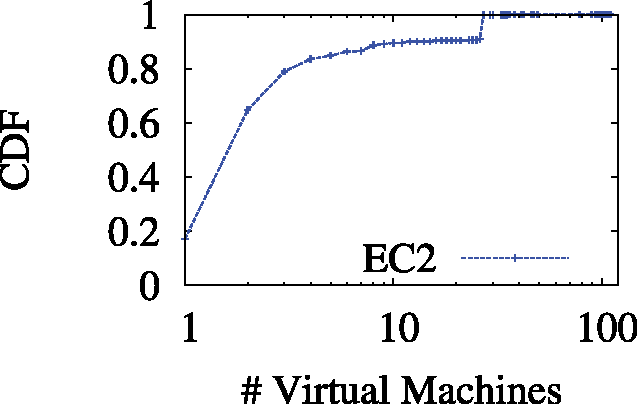
\includegraphics[width=\textwidth]{figures/cloudmeasure/imag_sec3/subdomain_vm_cdf.pdf}
    \label{fig:Alexa_ec2_non_elbs_CDF}
\end{subfigure}
\begin{subfigure}[b]{0.4\textwidth}
    \caption{Physical ELB instances}
    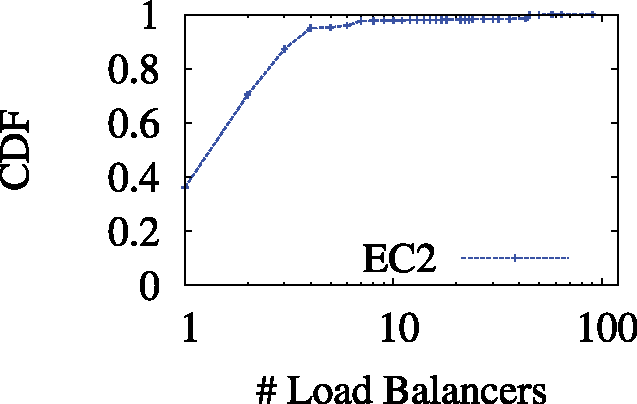
\includegraphics[width=\textwidth]{figures/cloudmeasure/imag_sec3/subdomain_elb_cdf.pdf}
    \label{fig:Alexa_ec2_elbs_CDF}
\end{subfigure}

\caption{CDFs for the \# of feature instances per subdomain (only includes
        subdomains which use the feature).}
\label{fig:Alexa_feature_CDF}
\end{figure}

\begin{figure}
    \centering
    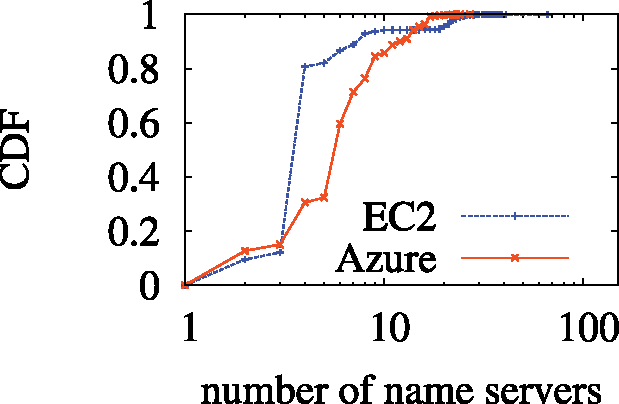
\includegraphics[width=0.50\columnwidth]{figures/cloudmeasure/imag_sec3/subdomain_ns_cdf.pdf}
    \caption{CDF of the \# of DNS servers used per subdomain.}
    \label{fig:Alexa_ns_subdomain_cdf}
\end{figure}



Aggregating by domain, we find that 52\% of EC2-using domains have at least
one subdomain which uses at least one \frontend VM. If we sum the number of
\frontend VMs used across all subdomains of a given domain, we find that 10\%
of domains which use \frontend VMs in EC2 use 3 or more \frontend VMs in
total. % (omitted for brevity).

\tightparagraph{PaaS \frontend in EC2} 
PaaS systems offer a hosted environment for deploying web applications, 
avoiding the need for tenants to manage low-level system details. PaaS
systems are frequently built atop existing IaaS infrastructure: e.g.,
Amazon's Elastic Beanstalk and Heroku
both run atop EC2. A Beanstalk environment always includes an Amazon Elastic
Load Balancer (ELB) instance (discussed in more detail below), reflecting
deployment pattern  {\em P2} (\figref{fig:ec2_elb}, replace
VMs with PaaS nodes). A Heroku environment may or may not include an ELB,
reflecting usage of deployment patterns {\em P2} or {\em P3}
(\figref{fig:ec2_models}), respectively.


We say that a subdomain uses Beanstalk or Heroku if the subdomain's DNS
record has a CNAME 
that ({\em i}) includes `elasticbeanstalk' or any of `heroku.com',
`herokuapp', `herokucom', and `herokussl' and ({\em ii}) resolves to
an IP in EC2's public IP address range. In the case of Heroku without ELB,
the IPs to which the CNAME resolves represent PaaS nodes; we associate these
IPs with the subdomain whose DNS record contains the corresponding CNAME.



 
A total of 201,666 (28\%) EC2-using subdomains in our \alexadata
dataset contain
a CNAME in their DNS record. Applying the above filters for PaaS, we
find that 60,273 (8\%) EC2-using subdomains use a \frontend PaaS
environment in EC2. Of these, over 97\% (59,991) are using Heroku;
only 3\% use Elastic Beanstalk. Amazon always includes an ELB in a  
Beanstalk environment, but Heroku only sometimes leverages ELBs---only 3\% of
subdomains (1,850) which use Heroku also use ELB.
We therefore conclude that,
in the case of EC2, PaaS systems are predominantly used according to
deployment pattern {\em P3} (\figref{fig:ec2_paas}).

We now focus on the 58,141 (59,991 - 1,850) subdomains that use
Heroku without ELB. We find that these are associated with just
94 unique IPs. Although we have no insight into the number of worker
instances used by Heroku, this shows that Heroku is multiplexing PaaS
functionality among a relatively large number of subdomains: in
particular, we find that about one-third of subdomains using
Heroku share the CNAME `proxy.heroku.com'.
 
\tightparagraph{Load balancer \frontend in EC2} 
Load balancers divide traffic among a set of ``worker'' VMs or PaaS nodes, as
reflected in deployment pattern {\em P2} (\figref{fig:ec2_elb}).
Amazon Elastic Load Balancers (ELBs) are Amazon-managed
HTTP proxies. An EC2 tenant requests an ELB in a specific region and
subsequently associates VM instances, in one or more zones, with this ELB.
The ELB automatically round-robins requests among zones and among the VMs in
each zone.  In fact, traffic is routed to zone-specific ELB proxies by
rotating the order of ELB proxy IPs in DNS replies. ELB can also
be used with PaaS, as discussed above.  

When a subdomain uses an ELB, the subdomain's DNS record contains a
CNAME ending in `elb.amazonaws.com'; the
CNAMEs resolve to IP addresses for one or more ELB proxies.  We identify
ELB-using subdomains in our \alexadata dataset based on the presence of such 
CNAMEs; we refer to each distinct CNAME as a ``logical ELB
instance''. We also associate with the subdomain the IPs of the specific ELB
proxies to which the CNAME resolves; we refer to these as ``physical ELB
instances''.

We find that 27,154 (4\%) EC2-using subdomains use ELB as their \frontend.
Of the subdomains that use ELB, 280 (1\%) use it in the context of Elastic
Beanstalk and 1,850 (6.8\%) use it with Heroku.  Aggregating by domain, we
find that 9,851 (26\%) EC2-using domains use \frontend ELB(s).

Across all ELB-using subdomains, we observe 15,703 physical ELB instances
(i.e., distinct IPs associated with ELB CNAMEs).
Hence, while each subdomain has its own logical ELB(s), the
physical ELB proxies that perform the actual load balancing appear to
be shared across multiple, even unrelated, subdomains. In particular, we 
analyzed the number of subdomains per
physical ELB and found that $\approx$4\% of the physical ELB instances are
shared by 10 or more subdomains.% (details omitted for brevity).



\figref{fig:Alexa_ec2_elbs_CDF} shows a CDF of the number of physical ELB
instances associated with each subdomain; this CDF only includes subdomains
which use ELB. We observe that about 95\% of ELB-using subdomains are
associated with 5 or fewer physical ELB instances. A few ELB-using 
subdomains (e.g., dl.outbrain.com and m.netflix.com) use many
physical ELB instances: 58 and 90, respectively.

\iffalse
\tightparagraph{Front ends in Azure}
Azure's architecture differs from EC2 insofar as clients cannot distinguish
whether a web service uses a VM, PaaS, or load balancer
\frontend. In Azure, VMs and PaaS environments are both encompassed within
logical ``Cloud Services'' (CS). An individual CS may contain ({\em i}) a
single VM, ({\em ii}) a collection of related VMs, or ({\em iii}) a PaaS
environment.  Each CS is assigned a unique DNS name ending with
`cloudapp.net' and a corresponding public IP address.  
Traffic sent to this public IP goes through a transparent
proxy---which performs NAT and, optionally, load balancing---before directing
traffic to a VM or PaaS node.  Thus, a CS may reflect deployment patterns
{\em P1}, {\em P2} (with VMs or PaaS nodes), or {\em P3} (\figref{fig:ec2_models}), all of which appear
the same from a client perspective.

We examine the DNS records for Azure-using subdomains in the
\alexadata dataset to identify subdomains which use a CS (i.e., VM, PaaS, or
load balancer) \frontend.  If the DNS query for
an Azure-using subdomain either directly returns an IP address or
returns a CNAME ending in `cloudapp.net', then we say the subdomain
uses a CS \frontend. We associate the directly returned IP or the
CNAME, and its corresponding IP, with a CS instance.

A total of 1,153 (17\%) Azure-using subdomains directly resolve to an IP
address and 5,404 (82\%) Azure-using subdomains contain a CNAME in their DNS
record.  Applying the above filters for CS, we find that 4,581 (70\%)
Azure-using subdomains use a CS \frontend.  Aggregating by domain, we find that 57\% of Azure-using domains
have at least one subdomain which uses a CS \frontend. 

Azure also offers a unique feature (which has no parallel in EC2) for load
balancing across \frontends: Azure Traffic Manager
(TM) uses DNS to direct traffic to different CSs, which
may be spread across multiple regions.  TM can, based on a tenant's
preference, do performance-based load balancing (finding the CS closest to
the client), failover load balancing (picking the next active CS), or simple
round-robin load balancing.  When a subdomain uses TM, its DNS record
contains a CNAME ending in `trafficmanager.net', similar to ELB.  However, TM
performs all load balancing using DNS---unlike ELB which uses a combination
of DNS and physical proxies---so TM CNAMEs resolve directly to a CNAME for a
specific CS (e.g., `abc.cloudapp.net').  We find that only 100 (2\%)
Azure-using subdomains (corresponding to 52 domains) use TM. 


The aforementioned CNAME-based filters for ELB, Beanstalk, Heroku, CS,
and TM were not applicable to 116,323 (16\%) EC2-using
subdomains, and 1,938 (30\%) Azure-using subdomains. We are
investigating techniques to understand the deployment patterns
underlying these subdomains.
\fi

\tightparagraph{Content distribution networks}  We now focus on the use
of CDNs, which we illustrated in deployment pattern {\em P4}
(\figref{fig:ec2_cdn}). Note that CDNs can be employed alongside any of the
other three deployment patterns.

Both Microsoft and Amazon run their own CDNs, which we focus on
studying. Amazon's CloudFront CDN uses a
different public IP address range than the rest of EC2. Hence, we
determine if a subdomain uses CloudFront by observing if its DNS
records contain one or more IPs in CloudFront's IP range.
Azure's CDN uses the same IP address ranges
as other parts of Azure, so we detect whether a subdomain
uses the Azure CDN based on whether a subdomain's DNS records contain
CNAMEs with `msecnd.net'.

We find 7,622 subdomains (corresponding to 5,988 domains) use CloudFront and
68 subdomains (corresponding to 54 domains) use Azure's CDN. 
Despite the much smaller number of domains using Azure's CDN, there is
still a significant volume of traffic associated with msecnd.net
in our \capturedata dataset (\tabref{tab:topdomains}). Azure's CDN is clearly
being used within some Microsoft properties, perhaps to host embedded
content or cookies.


\tightparagraph{Domain name servers} The first step in accessing a
cloud-resident service is to resolve its name
(\figref{fig:ec2_models}). In what follows, we examine cloud-resident
subdomain's use of DNS, focusing on the extent to which they rely on
cloud providers for DNS services as well.

%  versus employing DNS hosted
% outside the cloud. 

We identifed the ``location'' of a cloud-using subdomain's
authoritative name server(s) as follows: For each DNS record
associated with a given subdomain in our \alexadata dataset, we
extract all the domains specified in the NS records. We then performed
a DNS lookup on each of these domains from 50 globally-distributed
PlanetLab nodes. We flushed and reset the cache of the local resolver
between each DNS lookup, and we added the `norecurse' flag to each
DNS query to minimize the influence of caching. We compare the
resulting IP addresses to the public IP address ranges for EC2,
CloudFront, and Azure.

We observe a total of 23,111 name servers supporting the 713K
cloud-using subdomains in our \alexadata dataset. Many subdomains use
the same name servers, leading to a smaller set of name servers than
subdomains. \figref{fig:Alexa_ns_subdomain_cdf} shows a CDF for the
number of name servers used by each cloud-using subdomain; we observe
that nearly 80\% of subdomains use 3 to 10 name servers. We
categorize the name servers as follows: 2,062 were hosted in
CloudFront, which appears to host Amazon's route53 DNS service as many
of these name servers had `route53' in their domain name; 1,239 were running
inside EC2 VM instances; 22 were hosted inside Azure VM instances
or Azure CS; and 19,788 were
hosted outside any of EC2, CloudFront, or Azure; 


\begin{table}[tb]
\centering
\small
\input{cloudmeasure_tables/tab_features_used}

\caption{Summary of cloud feature usage.
}
\label{tab:features-used}
\end{table}

The above analyses are summarized in \tabref{tab:features-used} which
shows how many (sub)domains in our \alexadata dataset use each cloud
feature. We also show the number of instances (identified by IP
address) of that feature. 


\begin{table}[t]
\centering
\small
\input{cloudmeasure_tables/tab_feature_usage_by_top_alexa}
\caption{Cloud feature usage for the highest ranked EC2-using domains (* indicates use
          of a CDN other than CloudFront).}
\label{top_alexa_domains_cf}
\end{table}

\tightparagraph{Analysis of top domains} As notable exemplars,
\tabref{top_alexa_domains_cf} gives a detailed breakdown of the cloud
feature usage of the most popular (according to Alexa rankings)
EC2-using domains. We observe that the majority of subdomains associated
with the top domains have VM or ELB \frontends. Of those using ELB
\frontends, amazon.com and fc2.com use ELB the most (i.e., there are more
physical ELB IPs associated with these domains).  Three of the top domains
have subdomains which use a CDN, but only one of these domains uses the
CloudFront CDN.

\tightparagraph{Summary and implications} In summary, we find that the
majority (71.5\%) of EC2-using subdomains use a VM \frontend
(deployment pattern {\em P1}); hence most EC2 tenants are using EC2 as a
true IaaS cloud. Only a small fraction use an ELB \frontend (3.8\%) or
PaaS \frontend (8.5\%).  Due to limited use, failures of value-added
features are unlikely to have a major impact on EC2-using subdomains.
In Azure, we are able to identify the usage of VM, PaaS, or load
balancing \frontends (we cannot distinguish which) for 70\% of
subdomains.  A small fraction (1.5\%) of Azure-using domains leverage TM to
balance traffic across different \frontends. The majority of DNS
servers used by cloud-using subdomains reside outside of EC2 or Azure,
giving subdomains the option of routing traffic to different resources
(in another cloud or a private data center) in the event of cloud
failure.




\subsubsection{Region Usage}
\label{cloud-measure-region}

EC2 and Azure give tenants the choice of using one or more
geographically distinct regions (i.e., data centers). Regions provide a
mechanism for robustness in the case of catastrophic failures, e.g.,
regional power or service
outages~\cite{AWSoutageOct2012,AWSoutageDec2012,netflixoutage,wsjarticle}. In this section, we examine how many, and
which, of the eight regions offered by each cloud provider are
leveraged by the front ends of cloud-using (sub)domains.

We ascertain the region(s) used by each subdomain in the \alexadata dataset 
by comparing the IP addresses associated with that subdomain against the
per-region IP address ranges published by EC2~\cite{ec2iprange} and
Azure~\cite{azureiprange}. We only consider IPs associated with VM, PaaS, 
and ELB/TM. 
%%%%%%%%%%%%%%%%%%%%%%%%%%%%%%%%%%%%%%%%%%%%%%%%%%%%%%%%%%%%%%%%%%%%%%%%%%%%%

\figref{fig:cloud_region_subdomains_CDF} shows a CDF (note the Y-axis
starts at 90\%) of the number of regions used by each subdomain in
the \alexadata. Over 97\% of EC2-using and 92\% of Azure-using subdomains
exclusively use one region. Across all domains
(\figref{fig:cloud_region_domains_CDF}), the trend of low region usage
is largely the same, although, the fraction of Azure-using
domains that only use one region (83\%) is smaller than the fraction
of subdomains that only use one region (92\%). 


%%%%%%%%%%%%%%%%%%%%%%%%%%%%%%%%%%%%%%%%%%%%%%%%%%%
\begin{table}[t]
\center\small
\input{cloudmeasure_tables/tab_regions_used_by_alexa_nopcap}
\caption{EC2 and Azure region usage \alexadata}
\label{tab:region-breakdown}
\end{table}

The number of (sub)domains (from the \alexadata) in
each region are shown in \tabref{tab:region-breakdown}.  We observe
that the usage of EC2 regions is heavily skewed towards a few regions:
74\% of EC2-using subdomains use {\em US East} and 16\% use {\em
  Europe West}. Azure, relatively speaking, has
a more even distribution of subdomains across regions, but each region
has significantly fewer subdomains.  The most used Azure regions are
{\em US South} and {\em US North}. 



\begin{figure}[tb]
\centering
        \begin{subfigure}[b]{0.40\textwidth}
                \centering
		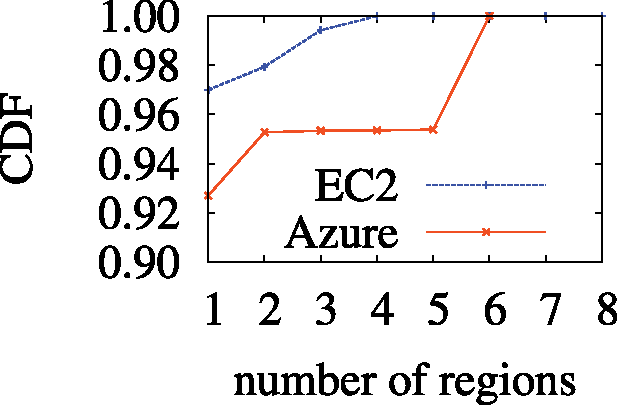
\includegraphics[width=\textwidth]{./figures/cloudmeasure/imag_sec4/region_cdf_new.pdf}
		\caption{subdomain}
		\label{fig:cloud_region_subdomains_CDF}
	\end{subfigure}
	\begin{subfigure}[b]{0.40\textwidth}
                \centering
                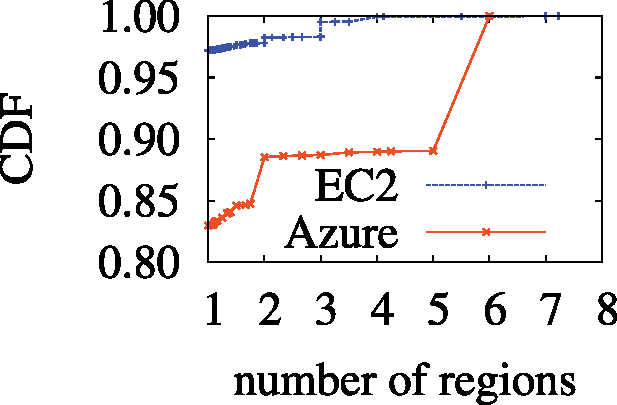
\includegraphics[width=\textwidth]{./figures/cloudmeasure/imag_sec4/region_cdf_new_avg.pdf}
		\caption{domain}
		\label{fig:cloud_region_domains_CDF}
	\end{subfigure}
\caption{(a) CDF of the number of regions used by each subdomain
(b) CDF of the average number of regions used by the subdomains of each domain.}
\label{fig:cloud_region_CDF}
\end{figure}


\begin{table}[t]
\centering
\small
\input{cloudmeasure_tables/tab_domain_deploy.tex}
\caption{Region usage for the top cloud-using domains. The third column 
is the number of cloud-using subdomains; fourth is the total number of 
regions used by a domain; and the $k=1$ and $k=2$ columns are the number of subdomains which
use one or two regions, respectively.}
\label{top_alexa_domains_deploy}
\end{table}



\tightparagraph{Analysis of top domains} We now focus on region usage of
subdomains corresponding to the most popular (according to Alexa
rankings) domains. Our analysis is summarized in
\tabref{top_alexa_domains_deploy}. As with the rest of our results
above, we see that in all but two cases, subdomains appear to use a
single region. The exceptions are msn.com and microsoft.com, where 11
of the 89 subdomains and 4 of 11 subdomains, respectively, use two
regions each. No popular subdomain uses three or more regions. We also
note that in some cases, a domain may deploy different subdomains
across different regions: e.g., live.com's 18 subdomains are spread
across 3 regions. Contrarily, there are domains whose subdomains 
are all deployed in one region (e.g., pinterest.com).

%\textcolor{red}{the following para is newly added!!!}


\tightparagraph{Analysis of subdomain deployment vs. customer location} An
interesting question about cloud service deployment is whether subdomains
are deployed near their customers? The answer to this question reveals whether
current cloud services are deployed in an ``optimal'' manner, because
deploying a service near customers usually leads to better client network 
performance (lower latency and higher throughput). 

To answer this question, we leverage the client geo-location information
provided by the Alexa web information service~\cite{alexawebinfo}.  For
example, at the time of writing, Alexa reported that 47\% of clients
accessing pinterest.com are from the United States, 10.4\% from India, 3.2\%
from the United Kingdom, 3.1\% from Canada, and 2.1\% from Brazil.  For each
domain, we define the ``customer country'' as the country where the largest
fraction of clients are located. We assume the customer country is the
same for all of a website's subdomains, as Alexa does not track subdomains
separately. For instance, the United States is the customer country for
pinterest.com (and its subdomains) based on our definition.

We performed the analysis for all of the cloud-using subdomains (about 713K)
in our dataset.  Our measurement methodology was able to successfully
identify approximately 538K (75\% of the total) subdomains' customer
country.  We find that 252K (47\%) subdomains' customer country is not the 
same as the country where this subdomain is hosted.  Moreover, 174K (32\%)
subdomains are not even hosted on the same continent as the subdomains'
customer country.  This implies that a large fraction of web services are 
probably not deployed in an optimal manner in terms of network performance.
We suspect that the current deployment posture is affected by 
computing, storage, and network costs and/or how long the cloud
region has existed. In \secref{cloud-measure-performance}, we explore how much
opportunity exists for improving wide-area performance through changes in
region usage.


\tightparagraph{Summary and implications} Our key finding in this section is
that most popular domains and subdomains appear to be using a single
region. This has significant implications on both the robustness and
performance of cloud-using web services. From an availability
perspective, an outage of EC2's {\em US East} region would take down critical
components of at least 2.3\% of the domains (61\% of EC2-using
domains) on Alexa's list of the top 1 million websites. This is a
lower bound, as our results do not include dependencies between
domains.  
From a performance perspective, our analysis of web service
deployment and customer locations reveals that a considerable fraction of
client traffic may travel farther than necessary due to suboptimal
provisioning.


\subsubsection{Availability Zone Usage}
\label{cloud-measure-zone}


Within each region of EC2, cloud tenants have the choice of deploying
across multiple zones. EC2 zones offer a means for improving service
robustness as they are claimed to use separate compute, network, and
power infrastructure so that a failure in any of these will not affect
more than one zone. There seems to be no
equivalent of zones in Azure.

We now focus on determining the zone deployment for
EC2-using services' front ends. Unlike the regions, which are easily
distinguished based on the IP address of a subdomain and the
advertised ranges~\cite{ec2iprange,azureiprange}, there is no direct way to associate an IP address
to a zone.  We therefore turn to cloud cartography
techniques~\cite{ristenpart2009hey}. We use two methods to identify
zones: network latency and proximity in the internal addresses to
instances with a known zone (i.e., VMs we launched).
Details about the two methods are presented in~\cite{he2013next}.
We combine the two zone identification methods to maximize the fraction of
physical instances whose zone we can identify.  We give preference to our
address-proximity-based zone identifications, and use our latency-based
identifications only for instances whose zone cannot be identified
using the former method.  Combining the two methods allows us to identify the
EC2 availability zone for 87.0\% of all physical EC2 instances in the
\alexadata dataset.

%\setlength{\tabcolsep}{0.1cm}
\begin{table}[t]
\center
\small
\begin{tabular}{|l||r|r|r|r|r|r|r|}
\hline
\bf Region & \multicolumn{2}{|c|}{1$^\textbf {st}$ \bf zone} &   \multicolumn{2}{|c|}{2$^\textbf {nd}$ \bf zone}   & \multicolumn{2}{|c|}{3$^\textbf {rd}$ \bf zone}  \\
           &\#Dom& \#Sub  & \#Dom& \#Sub & \#Dom& \#Sub\\
\hline
\awseast &  16.1  &  419.0&  6.2  & 155.4& 9.5  &  292.9 \\
\awscali &  1.6 &  33.2&  3.0  &  37.4 & N/A  &  N/A\\
\awsoreg  &  0.9 &  13.4 & 1.0 &  9.6 &0.8 &  7.3 \\
\awseuro  &   2.3  &  77.0&  2.9 & 63.9 & 4.5  &  98.7\\
\awstokyo &   0.4 & 3.7 & 1.3 & 11.3   &1.5 & 12.9 \\
\awssing  &  0.9 & 11.3 &   1.2 & 19.1 & N/A & N/A\\
\awssyd  &  0.2 & 0.3 & 0.2 & 0.3  & N/A & N/A \\
\awssp   &  0.5 & 14.4 &  0.2 & 8.9 & N/A & N/A\\
\hline
\end{tabular}
\caption{Estimated number of domains and subdomains using various EC2  zones. 
Some regions only have 2 zones.}
%Note there are only two zones in \awscali, \awssing, \awssyd and \awssp; there are three zones in \awstokyo, but we can only set up instances in two of them from Feb, 2013}
\label{tab:ec2-zone-usage}
\end{table}


\begin{figure}[!tb]
\centering
	\begin{subfigure}[b]{0.4\textwidth}
                \centering
                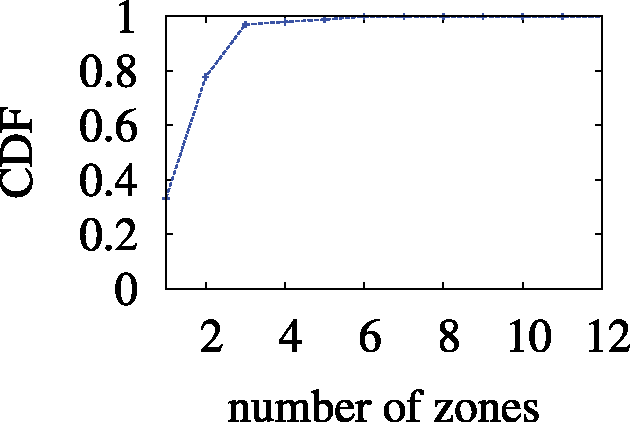
\includegraphics[width=\textwidth]{./figures/cloudmeasure/imag_sec4/zone_cdf_new_fix.pdf}
		\caption{subdomain}
		\label{fig:cloud_zone_subdomains_CDF}
	\end{subfigure}
	\begin{subfigure}[b]{0.4\textwidth}
                \centering
                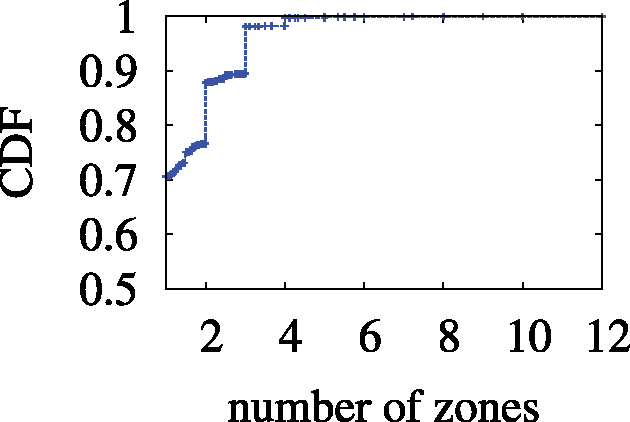
\includegraphics[width=\textwidth]{./figures/cloudmeasure/imag_sec4/avg_zone_cdf_new_fix.pdf}
		\caption{domain}
		\label{fig:cloud_zone_domains_CDF}
	\end{subfigure}
\caption{(a) CDF of the number of zones used by each subdomain 
(b) CDF of the average number of zones used by the subdomains of each domain.}
\label{fig:cloud_zone_CDF}
\end{figure}

\begin{table}[t]
\centering
\small
\input{cloudmeasure_tables/tab_domain_deploy_zone.tex}
\caption{Zone usage estimates for top using zones. Column 4 is estimated 
total number of zones used by all
subdomains. Columns 4--6 indicate the estimated number of subdomains that use 
$k$ different zones.}
\label{top_alexa_domains_deploy_zone}
\end{table}


\tabref{tab:ec2-zone-usage} summarizes the number of (sub)domains using each region and
zone.  In all but one region (Asia Pacific Southeast 2), we
observe a skew in the number of subdomains using each zone in a region. Asia
Pacific Northeast and US East regions have the highest skew across their
three zones: 71\% and 63\% fewer subdomains, respectively, use the least
popular zone in those regions compared to the most popular zone.  

We also look at the number of zones used by each (sub)do-main.
\figref{fig:cloud_zone_subdomains_CDF} shows a CDF of the number of
zones used by each subdomain.  We observe that 33.2\% of
subdomains use only one zone, 44.5\% of subdomains use two zones, and 22.3\%
of subdomains use three or more zones.  Of the subdomains that use two or
more zones, only 3.1\% use zones in more than one region.  
%For example, if
%the one of the zones in the US East region failed, \fixme{XX\%, XX\%, and
%XX\%} of subdomains would be completely unavailable if the 1st, 2nd, or 3rd
%zones, respectively, failed.
\figref{fig:cloud_zone_domains_CDF} shows the average number of zones used by
the subdomains of each domain.  We observe that most domains (70\%) only use
one zone for all subdomains; only 12\% of domains use two or more zones per
subdomain on average.  

Even for the top EC2-using domains, a large fraction of their subdomains only
use a single zone (\tabref{top_alexa_domains_deploy_zone}). For example,
56\% of pinterest.com's EC2-using subdomains and 33\% of linkedin.com's are
only deployed in one zone.  

%\figref{az_num} breakdowns the number of availability zones deployed by
%EC2-using subdomains by region.

\tightparagraph{Summary and implications} Our two key findings in this section
are that ({\em i}) the majority of EC2-using subdomains only use one (33.2\%)
or two (44.5\%) zones, and ({\em ii}) the subdomains using a given EC2 region
are not evenly spread across the availability zones in that region. The former
implies that many EC2-using subdomains would be completely unavailable if a
single zone failed, and many others would be severely crippled: e.g., a
failure of \awseasta would cause 16.1\% of subdomains to be completely
unavailable.  Our later key finding implies that an outage of a particular
zone in a region may have a greater negative impact than an outage of a
different zone in the same region: e.g., a failure of \awseasta would impact
$\approx$419K subdomains, while a failure of \awseastb would only impact
$\approx$155K.





%%%%%%%%%%%%%%%%%%%%%%%%%%%%%%%%%%%%%%%%%%%%%%%%%%%%%%%%%%%%%%%%%%%%%%%%%%%%%%%%
\subsection{Wide-Area Performance and Fault Tolerance}
\label{cloud-measure-performance} 


Our results in the last section revealed that several services, even
highly ranked Alexa domains, appear to use only a single region or
even just a single availability zone.  In this section, we explore the
impact of these choices on web services' wide-area performance and
tolerance to failures.  We focus on EC2-using web services.


\subsubsection{Wide-area Performance} 


The choice of region(s) by a cloud service may impact performance in
at least two ways. First, clients' geo-distribution may
be poorly matched to particular regions; such clients may experience
poor latency and throughput compared to a more
judicious deployment. Second, there could be temporary changes in
which region performs best for a client due to 
congestion~\cite{akella2003empirical} or routing
problems~\cite{teixeira2004dynamics}.
%Deploying cloud services in multiple regions has the potential to help
%improve user experience here as well.

While the impact of diverse deployment of services (e.g., via CDNs)
has been previously studied in other
settings~\cite{krishnan2009moving}, we are unaware of any studies that
assess its impact for the available diversity of modern public IaaS
clouds. We therefore perform measurements to help us answer the
following two questions: ({\em i}) To what extent does the choice of region
impact performance experienced by clients of a web service? ({\em ii}) To
what extent does the use of multiple regions (or zones) improve the
client-perceived performance?


\tightparagraph{Latency measurements.}  To study per-region latency
performance, we set up 40 m1.medium instances, 2 in each of the 20
availability zones available to us on EC2. 
We selected 80 geographically distributed
PlanetLab~\cite{planetlab} nodes as stand-ins for real clients and we
used the hping3 utility to conduct 5 TCP pings to each of the 40
instances, from which we derive the average RTT. Pings that timed out
were excluded from the calculations of the average.
% The average RTT was computed as the average of these 5 pings; pings
% with 0 RTT were omitted from the calculation.
Probing was performed once every 15 minutes for three consecutive days.

\tightparagraph{Throughput measurements.} 
We used the same set of 40 m1.med\-ium EC2 instances and 80 PlanetLab nodes to
measure throughput. We divided the PlanetLab nodes into
two groups of 40. Each node in each group performed an HTTP get of
a 2\,MB file to one of the 40 EC2 instances (which were running Apache web
server). At any given time, only one HTTP connection was
established with each EC2 instance to avoid contention across
throughput measurements. In particular, the
clients in each group performed an HTTP get operation every 11.25
seconds; the download was canceled if it took more than 10 seconds.
Each client accessed all 40 servers in each round, which means it took
450 seconds for one group to finish a round of downloading the file
from each of the servers.  So, in total, it took 15 minutes for
80 clients to perform one round of throughput measurements.
The final throughput is measured as file\_size / download\_time.
We ran the measurements for three consecutive days, 
for a total of 288 data points per client. The throughput measurements
were intermingled with the latency measurements.


\begin{figure}[t]
\centering
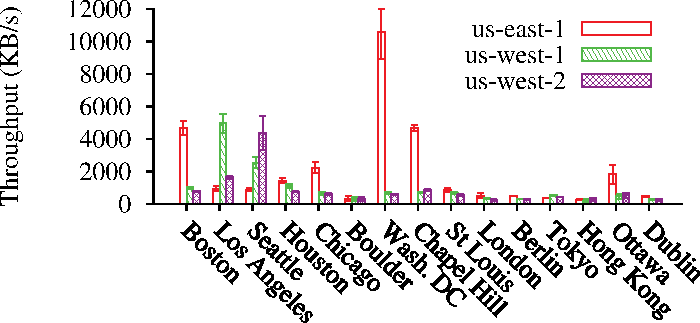
\includegraphics[width=0.55\textwidth]{./figures/cloudmeasure/imag_sec5/region_bandwidth.pdf}
\caption{Average throughput between representative clients and EC2 regions in the US.}
\label{fig:region_bandwidth}
\end{figure}

\begin{figure}[t]
\centering
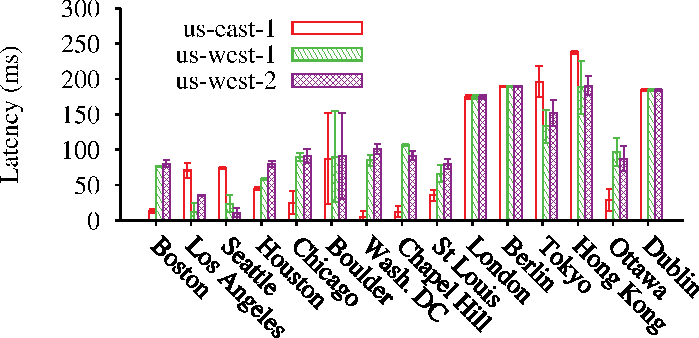
\includegraphics[width=0.55\textwidth]{./figures/cloudmeasure/imag_sec5/region_latency.pdf}
\caption{Average latency between representative clients and EC2 regions in the US.}
\label{fig:region_latency}
\end{figure}


\tightparagraph{Performance across different regions.}
Figures~\ref{fig:region_bandwidth} and \ref{fig:region_latency} show the
latency and throughput measurements for 15 representative PlanetLab
locations and for the three US EC2 regions. The PlanetLab nodes are spread
across the US and other parts of the world. 
%\tnote{How were these selected? Why is
%it different across the different charts?}
We make a few key observations: ({\em i}) Single-region deployments must
carefully choose a region. For example, the two US west
regions do not offer equivalent ``across-the-board'' performance, with
ec2.us-west-1 offering better average latency and throughput (130 ms
and 1143 KB/s) than ec2.us-west-2 (145 ms and 895 KB/s)
(averaged across all client locations). ({\em ii}) The charts show that the
region chosen to serve content to a given client can have a
significant performance impact. For example, for the client in
Seattle, using the ec2.us-west-2 region can reduce latency by close to
a factor of 6 and improve throughput by close to a factor of 5
compared to using ec2.us-east-1. ({\em iii}) We also note that the way a
region is chosen may depend on the client's location: always choosing
ec2.us-west-1 for the Seattle client is a good idea, but for the
client in Boulder, the best choice of region may change
dynamically.

\iffalse
\begin{figure}[!t]
\centering
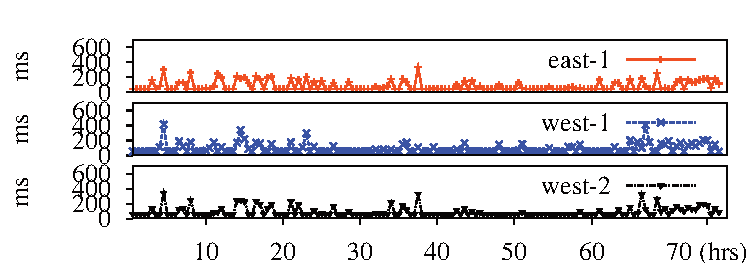
\includegraphics[width=0.55\textwidth]{./figures/cloudmeasure/imag_sec5/sec5_latency_colorado.pdf}
\caption{Latencies between Boulder site and three EC2 US regions. The
  best performing region changes over time.}
\label{fig:boulder_latency}
\end{figure}
\fi

We now examine the relative benefits of, and choices underlying,
multi-region deployments in more detail. We start by deriving an upper
bound on the performance from a $k$-region deployment of a service. To
do this, we determine the best $k$ regions out of the 8, for $1 \le k
\le 8$.  Using our measurement data we determine the overall
performance that the clients would have achieved given a routing
algorithm that picked the optimal region from the $k$ for each client
and at each point in time. More specifically, for each value of $k$
we: ({\em i}) enumerate all size-$k$ subsets of regions; ({\em ii}) for each
size-$k$ subset compute the average performance across all clients
assuming each client uses the lowest latency or highest throughput
region of the $k$ at each time round (15 min); 
and ({\em iii}) choose from these the size-$k$ subset with lowest latency or
highest throughput.
\figref{fig:multi_region_latency_bandwidth} shows the results. We find that while average performance can be increased a
significant amount by adding more regions to one's deployment, there
is evidence of diminishing returns after $k=3$. In particular, latency
decreases by 33\% when $k=3$ compared to $k=1$, but only decreases by
39\% when $k=4$.

We now examine what constitutes the best $k$ regions to use. The
choice of best regions, by throughput, is as follows: \awseast
($k=1$); \awseast ,\awseuro($k=2$); \awseast, \awseuro, \awscali
($k=3$); and \awseast, \awseuro, \awscali, \awssing ($k=4$).
%\tnote{This statement is a bit ambiguous. 
%Do we mean that it provided the highest on average across all regions?
%We should then answer the natural question of whether 
%people are using US East because it's so good (maybe push to a discussion 
%section later though).}  
The choice of best regions, by latency, is: \awseast
($k=1$); \awseast,\awstokyo ($k=2$); \awseast, \awstokyo, \awscali
($k=3$); and \awseast, \awstokyo, \awscali, \awssing ($k=4$).



\tightparagraph{Performance across different zones.} We also investigated the
difference in performance should one use different zones in the
same region. % \figref{fig:zone_bandwidth} and \figref{fig:zone_latency}
% give the latency and throughput for the three \awseast zones as seen
% from clients in 15 representative cities.
We found that the zone has
little impact on latency, with almost equivalent average RTTs for all
clients across the two days (results omitted for brevity). For throughput, the variation appears to
be somewhat higher, but not as significant as that seen across
regions. % For some periods in time, better throughput is seen to one
% zone than the other.
We believe such variation is due to local
effects, such as contention on shared instances or network
switches. % \tnote{The implications are stronger in that the averages
%   over time are also different, at least for the Boston
%   example. Should we say so or is it too slight to be significant?}
% \aditya{seems small to me..} 
This is suggested as well by other
recent measurements of EC2 performance
variability~\cite{farley:gaming:socc:2012}.  Moreover, in the next
section we show that the Internet path variability between zones is
low as well.

\tightparagraph{Summary and Implications} We find that using multiple
regions can improve latency and throughput significantly. However,
leveraging multiple regions may not be easy: while a given region
always offers best performance for some clients, the choice of region
for other clients will have to adapt in an online dynamic
fashion. This could be achieved via global request scheduling (effective,
but complex) or requesting from multiple regions in parallel (simple,
but increases server load).

While a multiple region deployment helps improve web service 
performance and protects against major cloud failures, cloud tenants must
also consider other factors in making their decision of how many and which
regions to use. First, cloud providers charge for inter-region network
traffic, potentially causing tenants to incur additional charges when
switching to a multi-region deployment. Second, the design of particular
cloud features may restrict how a tenant's data can be shared across regions:
e.g., objects stored in Amazon's Simple Storage Service (S3) can only be
stored in one region at a time and Amazon Machine Images (AMIs) cannot be
shared between regions. Lastly, deployments that rely on fewer features may be
less susceptible to failures---e.g., deployments which only use VMs, and not
other services like Amazon Elastic Block Storage or Amazon ELB, have not been
affected by some major 
outages~\cite{AWSoutageOct2012,AWSoutageDec2012}---reducing the need for resiliency through the use of multiple regions.


\begin{figure}[tb]
\centering
	\begin{subfigure}[b]{0.4\textwidth}
                \centering
                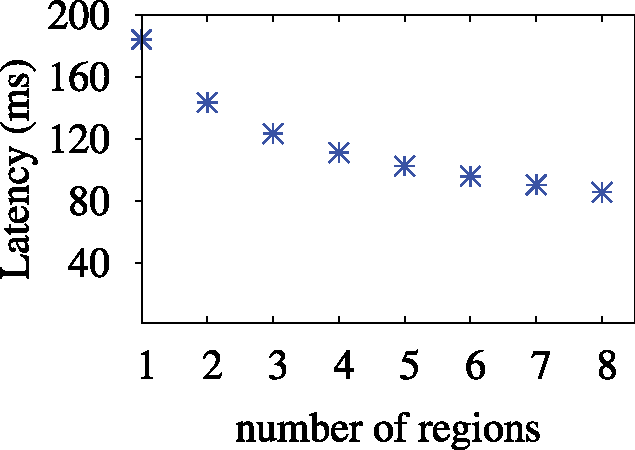
\includegraphics[width=\textwidth]{./figures/cloudmeasure/imag_sec5/sec5_region_latency_impr_fix.pdf}
		\caption{Latency}
	\end{subfigure}
	\begin{subfigure}[b]{0.4\textwidth}
                \centering
                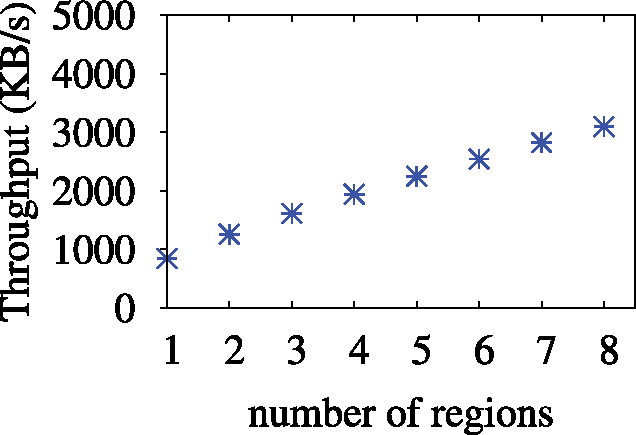
\includegraphics[width=\textwidth]{./figures/cloudmeasure/imag_sec5/sec5_region_speed_impr_fix.pdf}
		\caption{Throughput}
	\end{subfigure}
	\caption{Average latency/throughput across all clients using an optimal $k$-region
	deployment.}
	\label{fig:multi_region_latency_bandwidth}
\end{figure}

\subsubsection{ISP Diversity}

We now investigate tolerance to wide-area faults. Having in previous sections
already established the reliance of many cloud-using services on one zone or region,
we now focus on diversity in the immediate downstream ISPs at each EC2 zone. Greater
diversity, and an even spread of routes across downstream ISPs,
generally indicates greater tolerance to failures in Internet routing.

\begin{table}[t]
\centering\small
\begin{tabular}{|c||c|c|c|} \hline
\bf Region & \bf AZ1 &  \bf AZ2 &  \bf AZ3  \\ \hline
ec2.us-east-1 &  36 & 36 & 34\\ \hline
ec2.us-west-1 & 18 & 19 & n/a\\ \hline
ec2.us-west-2 &  19 & 19 & 19\\ \hline
ec2.eu-west-1&  10 & 11 & 13\\ \hline
ec2.ap-northeast-1 & 9 & n/a & 9\\ \hline
ec2.ap-southeast-1 &  11 & 12 & n/a\\ \hline
ec2.ap-southeast-2&    4 & 4 & n/a\\ \hline
ec2.sa-east-1 &  4 & 4& n/a\\ \hline
\end{tabular}

\caption{Number of downstream ISPs for each EC2 region and zone.}
\label{as_number}
\end{table}

To do this study, we set up three m1.medium instances in each of the
available EC2 availability zones.  Then we ran \emph{traceroute}
50 times from each of these instances to each of 200 geographically
diverse PlanetLab nodes (\figref{fig:nodes_deploy}).  Finally, we used
the UNIX `whois' utility to
determine the autonomous system (AS) number associated with the first non-EC2
hop, and we count that AS as an immediate downstream ISP for the zone hosting 
the instance. The discovered ASs constitute a lower bound for the true number of ASs.
\tabref{as_number} gives the number of distinct
ASs seen for each zone and region.
We note that:
({\em i}) different zones in a region have (almost) the same number of
  downstream ISPs; and
({\em ii}) the extent of diversity varies across regions, with some
  connected to more than 30 downstream ISPs and others
  connected to just 4. Except for South America and Asia Pacific
  Sydney, other regions are well-multihomed.


We also studied the spread of routes across downstream ISPs (not
shown). We found it to be rather uneven: even when using
well-connected regions -- e.g., \awscali and \awseuro -- we found that
up to 31\% (\awscali) and 33\% (\awseuro) of routes use the same
downstream ISP.

\tightparagraph{Summary and Implications} Although individual regions are
multihomed, the uneven spread of routes implies that local failures in
downstream ISPs can cause availability problems for large fractions of
clients of cloud-using web services. This could be overcome by using
multiple regions at once, or by leveraging dynamic route control
solutions~\cite{akella2004multihoming}.

%%%%%%%%%%%%%%%%%%%%%%%%%%%%%%%%%%%%%%%%%%%%%%%%%%%%%%%%%%%%%%%%%%%%%%%%%%%%%%%%


%\subsection{Conclusion}
\label{cloud-measure-conclusion}

In this work we performed the first extensive measurement study of
usage of modern infrastructure-as-a-service (IaaS) clouds, in
particular Amazon EC2 and Windows Azure. This measurement study, which combined data
from a university packet capture, interrogation of DNS records for
websites listed on the Alexa top 1 million list, and lightweight
probing, confirms the oft-reported anecdotes about the extent to which
modern web services use these cloud systems.  We profile the
deployment patterns observed for popular web services.  We uncover
that, in many ways, these deployments are somewhat precarious, as the
vast majority of (even very popular) websites use only one cloud
region.  In addition to resiliency benefits, we show that multi-region
deployments could significantly increase latency and throughput
performance in EC2.
Beyond providing a snapshot on the state of cloud usage, we
believe our work will spark further research on 
tracking cloud usage, as well as developing 
cloud-region-aware routing and deployment mechanisms.
Finally, we make all data sets used in 
this paper publicly available~\cite{cloudmeasuredata}, with the
exception of the \captureonedata.


\section{Proposed Work}
\label{plan}

\subsection{Congestion control enforcement for low latency datacenter networks}

\iffalse
There are many practical performance hurdles when we build high throughput and low latency data center 
networks to accommodate high-demanding applications 
(\eg{}, in-memory computing needs fast network to finish computing tasks). 
DCTCP~\cite{alizadeh2011dctcp} is a transport protocol designed to reduce the network buffering 
(thus reducing network latency) for data center networks. But, as we learned, 
in a real production data center network, it is hard to assume that all the TCP stacks are 
under the cloud provider's control. This is the case for infrastructure-as-a-service (IaaS) cloud, \eg{}, 
the default TCP protocol used by Amazon EC2 instances is TCP CUBIC at the time of writing. 
From the cloud provider's view, first, 
we want to achieve the goal of low latency for all of the tenant's traffic. Therefore, 
there is a need to enforce DCTCP-like transport protocol on every host in the network. 
Second, applying DCTCP’s ECN setting to data center switches seriously harms traditional TCP traffic.
As pointed out by~\cite{judd2015dctcp}, when TCP traffic is mixed with DCTCP traffic and ECN marking
is turned on, there are two practical performance issues: 1)DCTCP can gain almost all
the bandwidth while TCP can only get very little share and 2)TCP or DCTCP's connection
establishment probability is decreased sharply with the increase of the number of
competing flows in the network. All these two issues are related to the switch's
AQM (Active Queue Management) scheme---it simply drops non-ECT (ECN-Capable Transport)
packets when the switch's queue length is (even slightly) larger than the threshold.
One of the solutions is to apply ECT to all packets at the virtualization edge
(no matter it is TCP CUBIC or DCTCP, no matter it is control packets or data packets).
We undo the ECT marking properly when the packet arrives the destination host.
We propose to build a universal congestion control enforcement component in the virtualization layer or the NIC to 
boost the network performance (both low latency and high throughputs) for all kinds of traffic. 
The major challenge in achieving this goal is how we can solve this problem in a scalable and light-weight manner. 
We plan to implement this congestion control enforcement component on a real testbed and 
run various kinds of tests to validate its performance.
Finally, we also hope that our congestion control enforcement
logic is beneficial to the lossness \emph{ Data Center Bridging } or \emph{ Converged Ethernet }
environment where there are serious bufferbloat (hence increased network latency) and
fairness issues~\cite{tcp-bolt,zhu2015rdma}.
It can also improve the network performance for over-conservative transport protocols such as TCP+ECN.
\fi

Multi-tenant datacenters are a crucial component of today's computing ecosystem. Large providers, such as Amazon, Microsoft, IBM, Google and Rackspace, support
a diverse set of customers, applications and systems through their public cloud offerings. These offerings are successful in
part because they provide efficient performance to a wide-class of applications running on a diverse set of platforms. Virtual
Machines (VMs) play a key role in supporting this diversity by allowing customers to run applications in a wide variety of
operating systems and configurations.

And while the flexibility of VMs allows customers to easily move a vast array of applications into the cloud, that same flexibility inhibits the
amount of control a cloud provider can yield over VM behavior. For example, a cloud provider may be able to provide virtual networks or enforce rate limiting
on a tenant VM, but it cannot control the TCP/IP stack running on the VM. As the TCP/IP stack considerably impacts overall network performance, it
is unfortunate that cloud providers cannot exert a fine-grained level of control over one of the most important components in the networking stack.

Without having control over the VM TCP/IP stack, datacenter networks remain at the mercy of inefficient, out-dated or misconfigured TCP/IP stacks.
TCP behavior, specifically congestion control, has been widely studied and many issues have come to light when its behavior is not optimized. For example,
network congestion caused by non-optimzed stacks can lead to loss, increased latency and reduced throughput.

Thankfully, recent advances in optimizing TCP stacks for datacenter environments have shown that both high throughput and low latency can be
achieved through novel TCP congestion control algorithms. Works such as DCTCP~\cite{alizadeh2011dctcp} and TIMELY~\cite{mittal2015timely} show great promise in providing high
bandwidth and low latency by ensuring that network queues in switches do not fill up. And while these stacks are deployed in many of today's
private datacenters~\cite{singh2015jupiter,judd2015dctcp}, ensuring that a vast majority of VMs within a public datacenter will update their TCP stacks
to this new technology is a daunting, if not impossible task.

We plan to explore how operators can regain control of TCP's congestion control, regardless of the TCP stack
running in a VM. Our aim is to allow a cloud provider to utilize advanced TCP stacks, such as DCTCP, without having
control over the VM or requiring changes in network hardware. We propose implementing congestion control in the virtual switch
(vSwitch) running on each server. Implementing congestion control within a vSwitch has several advantages.
First, vSwitches naturally fit into datacenter network virtualization architectures and are widely
deployed~\cite{pfaff2015design}. Second, vSwitches can easily monitor and modify traffic passing through them.
Today vSwitch technology is mature and robust, allowing for a fast, scalable,
and highly-available framework for regaining control over the network.

Implementing congestion control within the vSwitch has numerous challenges. First, in order to ensure adoption rates are high, the
approach must work without making changes to VMs.
Hypervisor-based approaches that do not modify VMs typically rely on rate limiters to limit VM traffic. Rate limiters implemented in
commodity hardware do not scale in the number of flows and software implementations incur high CPU overhead~\cite{radhakrishnan2014senic}.
Therefore, limiting a VM's TCP flows in a fine-grained, dynamic nature
at scale (10,000's of flows per server~\cite{moshref2013vcrib}) with limited computational overhead remains challenging.
Finally, VM TCP stacks may differ in the features they support (\eg{}, ECN) or the congestion
control algorithm they implement, so a vSwitch congestion control implementation should work under a variety
of conditions.

We propose a new technology that implements
TCP congestion control within a vSwitch to help ensure VM
TCP performance cannot impact the network in an adverse way. At a high-level, the vSwitch monitors all packets for a flow, modifies
packets to support features not implemented in the VM's TCP stack (\eg{}, ECN) and reconstructs
important TCP parameters for congestion control. vSwitch runs the congestion control logic specified by an administrator and then enforces an intended
congestion window by modifying the receiver advertised window (\rwnd{}) on incoming ACKs. A policing
mechanism (\ie{}, via dropping any excess packets not allowed by the calculated congestion window) ensures stacks cannot benefit from ignoring~\rwnd{} and can also be used for non-TCP traffic.

\subsection{Datacenter network architecture analysis and exploration}

Datacenter network architecture determines how scalable the network is, 
how resilient it is to link or switch failures and how easily the network 
can be incrementally deployed. Today's practice is that network architect needs to 
manually infer (usually based on experiences) many key characteristics related to 
the candidate network topologies. So we lack a scientific and complete method to 
evaluate different network topologies. Therefore, there is a need to build a network 
architecture analysis framework to help network architect analyze and compare 
candidate network topologies. To compare different network topologies, we need to 
set up metrics to quantify different network topologies. Our first goal is to 
identify a set of metrics (e.g., cost, wiring complexity, bandwidth, reliability, routing convergence) that 
can accurately quantify datacenter network topologies.  Also, we need to define a set of workloads 
and traffic patterns to run against the network. Given the metrics and workloads, 
we are very interested to answer questions like: how many hosts are disconnected when 
a TOR switch fails? How much bandwidth is lost when an aggregation switch fails? 
When a core switch fails? What about specific links? 

Analyzing the existing topologies such as VL2~\cite{vl2}, FatTree~\cite{fattree}, F10~\cite{liu2013f10}, 
Jupiter~\cite{singh2015jupiter} is our first step. Next, we want to investigate that using 
this analysis framework, whether we can gain insights to design better network topologies. 
A motivating example is F10, which identifies new striping patterns that can 
improve FatTree's fault-tolerance. Using our analysis framework, it will be much faster 
to explore new datacenter network topologies and exam the tradeoffs among different metrics 
for new topologies. Finally, we will investigate how we codesign routing protocol, 
load balancing schemes to best utilize the new topologies. 

\subsection{Timeline}

Table \ref{tab:plan} shows my plan for completion of the research.

\begin{table}[hc]
\begin{small}
\begin{center}
\begin{tabular}{lll}
Timeline & Work & Progress\\
\hline
          & Presto \& CloudMeasure & completed\\
Oct 2016 & congestion control enforcement (NSDI'16) & proposed\\
Jan 2017 & datacenter network architecture analysis and exploration (SIGCOMM'17)  & proposed\\
May 2017 & thesis defense & \\
\end{tabular}
\end{center}
\end{small}
\caption{Plan for completion of my research}
\label{tab:plan}
\end{table}



\pagebreak

\begin{footnotesize}
\bibliographystyle{abbrv}
\bibliography{refer}
\end{footnotesize}

\end{document}


